\documentclass[preprint,nocopyrightspace]{sigplanconf-pldi16}

\usepackage{caption}
\DeclareCaptionType{copyrightbox}

\usepackage{amsmath,amsthm,amssymb,stmaryrd}
\usepackage{graphicx}
\usepackage{epstopdf}
\usepackage{MnSymbol}
\usepackage{paralist}
\usepackage{epsfig}
\usepackage{wrapfig}
\usepackage{color}
\usepackage{program}
\usepackage{url}
\usepackage{multirow}
\usepackage{rotating}
\usepackage{subfig} 
\usepackage{proof}
\renewcommand*{\proofname}{Proof Sketch}
\usepackage{hyperref}
%\usepackage[normalem]{ulem}
\usepackage{harpoon}
\usepackage{galois}



\usepackage{supertabular}

\newcommand\op{o\!p}
\newcommand\PMPY{Push/Pull}
\newcommand\PMPYfoot{\footnote{\scriptsize %
  \url{http://en.wikipedia.org/wiki/List\_of\_Doctor\_Dolittle\_characters\#The\_Pushmi-pullyu}}}
\newcommand\Ops{\text{\it O\!p\!s}}
%\newcommand\crit[2]{\underline{\text{#1 \emph{Crit.} (\emph{#2})}}}
%\newcommand\crit[2]{\text{\emph{\bf Crit}\ #1 (\emph{#2}){\bf .}}}
\newcommand\crit[2]{#1 criterion (\emph{#2})}
\newcommand\critAPPi{\crit{\APPLY{}}{i}}
\newcommand\critAPPii{\crit{\APPLY{}}{ii}}
\newcommand\critAPPiii{\crit{\APPLY{}}{iii}}
\newcommand\critPUSHi{\crit{\PUSH{}}{i}}
\newcommand\critPUSHii{\crit{\PUSH{}}{ii}}
\newcommand\critPUSHiii{\crit{\PUSH{}}{iii}}
\newcommand\critUNPUSHi{\crit{\UNPUSH{}}{i}}
\newcommand\critUNPUSHii{\crit{\UNPUSH{}}{ii}}
\newcommand\critPULLi{\crit{\PULL{}}{i}}
\newcommand\critPULLii{\crit{\PULL{}}{ii}}
\newcommand\critPULLiii{\crit{\PULL{}}{iii}}
\newcommand\critUNPULLi{\crit{\UNPULL{}}{i}}
\newcommand\critCMTi{\crit{\CMT{}}{i}}
\newcommand\critCMTii{\crit{\CMT{}}{ii}}
\newcommand\critCMTiii{\crit{\CMT{}}{iii}}
\newcommand\critCMTiv{\crit{\CMT{}}{iv}}
\newcommand\tx[1]{\texttt{tx}\ #1}
\newcommand\skipt{\texttt{skip}}
\newcommand\plust{\;\texttt{+}\;}
\newcommand\semit{\;\texttt{;}\;}


\newcommand\TRUE{\textsf{true}}
\newcommand\FALSE{\textsf{false}}

\newcommand\APPLY{{\sc apply}}
\newcommand\UNAPP{{\sc unapply}}
\newcommand\PUSH{{\sc push}}
\newcommand\UNPUSH{{\sc unpush}}
\newcommand\PULL{{\sc pull}}
\newcommand\UNPULL{{\sc unpull}}
\newcommand\CMT{{\sc cmt}}

\newcommand\gCommitted{\textsf{gCmt}}
\newcommand\gUncommitted{\textsf{gUCmt}}

\newcommand\lPushed{\small\textsf{pushed}}
\newcommand\lUnpushed{\small\textsf{unpushed}}
\newcommand\lPulled{\small\textsf{pulled}}
\newcommand\lCommitted{\small\textsf{cmted}}

\newcommand\x{\texttt{x}}
\newcommand\y{\texttt{y}}

\newcommand\pmpyreduce{\rightsquigarrow}

\newcommand*{\mystrut}{\rule[-0.05\baselineskip]{0pt}{1.15\baselineskip}}
%\newcommand\Tboxed[1]{\fbox{\mystrut #1}}
\newcommand\Tboxed[1]{#1}

%\newcommand\pmpyreduce{\xrightarrow{\;\;\;}}
%\newcommand\pmpyrt{\xrightarrow{\textsf{rt}}}
%\newcommand\pmpyfwd{\xrightarrow{\textsf{fwd}}}
%\newcommand\pmpyback{\xrightarrow{\textsf{back}}}
%\newcommand\pmpystruct{\xrightarrow{\textsf{struct}}}


%!TEX root=paper.tex

\newcommand\opname{m}
%\newcommand\step[1]{\textsf{step}(#1)}
\newcommand\nothingtext{fin}
\newcommand\nothing[1]{\textsf{\nothingtext}(#1)}
\newcommand\committ{\textsf{cmt}}
\newcommand\lstack{\sigma}
\newcommand\opid{\mathit{id}}
\newcommand\fresh[1]{\textsf{fresh}(#1)}
\newcommand\OPL{\ell} 
\newcommand\unpushed[1]{\lfloor #1 \rfloor_{\lUnpushed}}
\newcommand\pushed[1]{\lfloor #1 \rfloor_{\lPushed}}
\newcommand\mine[1]{\lfloor #1 \rfloor^{\lUnpushed}_{\lPushed}}
\newcommand\pulled[1]{\lfloor #1 \rfloor_{\lPulled}}
\newcommand\gcommitted[1]{\lfloor #1 \rfloor_{\gCommitted}}
\newcommand\guncommitted[1]{\lfloor #1 \rfloor_{\gUncommitted}}


\newcommand\SimRel{\;\sim\;}
\newcommand\theOP{\langle m, \sigma, \sigma', \opid \rangle}
\newcommand\numOP[1]{\langle m_#1, \sigma_#1, \sigma'_#1, \opid_#1\rangle}
\newcommand\cmtpres{\textsf{cmtpres}}
\newcommand\prewind{\;\circlearrowleft_\textsf{self}\;}
\newcommand\Gpost{G_\textsf{post}}
\newcommand\CSL{\{c, \sigma, L\}}
\newcommand\CSLp{\{c, \sigma, L'\}}
\newcommand\CpSpLp{\{c', \sigma', L'\}}
\newcommand\csL[1]{\{c, \sigma, #1\}}
\newcommand\cslC[1]{\{#1, \sigma, L\}}
\newcommand\cslCS[2]{\{#1, #2, L\}}
\newcommand\cslCSL[3]{\{#1, #2, #3\}}
\newcommand\cslpre{\{`c, `\sigma, `L\}}
\newcommand\cslhat{\{\hat{c}, \hat{\sigma}, \hat{L}\}}

%\newcommand\Gdrop{G_\textsf{drop}}
\newcommand\Gdrop{`G}
\newcommand\Godrop{`{}`G}
\newcommand\Grewindt[1]{\circlearrowleft_{\!\!\!#1}}
\newcommand\Grewind[3]{#1 \; \Grewindt{#2} #3}
\newcommand\GrewindGLGdrop{\Grewind{G}{L}{\Gdrop}}
\newcommand\GrewindGLGodrop{\Grewind{G}{L}{\Godrop}}

\newcommand\Gothers{\Gpost\setminus \pushed{L_1\cdot\hat{L}_2}}
\newcommand\Gmine{\Gpost\cap \pushed{L_1\cdot\hat{L}_2}}
\newcommand\GothersP{\Gpost'\setminus \pushed{L_1\cdot\hat{L}_2}}
\newcommand\GmineP{\Gpost'\cap \pushed{L_1\cdot\hat{L}_2}}

%\newcommand\invA{\textsf{inv}_a}
\newcommand\invLG{I_{LG}}
\newcommand\invA{I_\textsf{slideR}}

\newcommand\invSlidePushed{I_\textsf{slidePushed}}
\newcommand\invB{I_\textsf{reorderPUSH}}
\newcommand\invChronPush{I_\textsf{chronPush}}
\newcommand\early[3]{\textsf{early }#1\textsf{ than }#2\textsf{ in }#3}

\newcommand\invC{I_\textsf{localOrder}}

\newcommand\invNA{I_\textsf{RightOfPulled}}
\newcommand\invNB{I_\textsf{movePulledLeft}}

\newcommand\origtx{\textsf{otx}}

% %%%% params: c s L G
% \newcommand\invar[4]{\begin{array}{ll}%
%     \forall \cslpre.\ \cslCSL{#1}{#2}{#3} \prewind \cslpre \;\Rightarrow&(1)\\%
%     \forall \Gpost.\ \committ(#4,`L,\Gpost) \;\Rightarrow&(2)\\%
%     \forall \sigma',\OPL_a.\ (`c, `\sigma), \gcommitted{\Gpost}\cdot\unpushed{`L} \;\Downarrow\; \sigma', \OPL_a \;\Rightarrow&(3)\\%
%     \;\;\exists \OPL_b.\;\;\;%
%        \origtx(\cslpre), \gcommitted{#4} \Downarrow  \sigma', \OPL_b%
%        \;\;\;\wedge\;\;\;  \OPL_a \opeq \OPL_b\hspace{0.1in}&(4)%
%   \end{array}}
% \newcommand\invarCSLG{\invar{c}{\sigma}{L}{G}}

\newcommand\invLocalReorder{I_\textsf{localReorder}}

%%%% params: c s L G
\newcommand\invar[4]{\begin{array}{ll}%
    \forall \Godrop.\ \Grewind{#4}{L}{\Godrop}. \;\Rightarrow&(0)\\%
    \forall \cslpre.\ \cslCSL{#1}{#2}{#3},\Godrop \prewind \cslpre,\Gdrop \;\Rightarrow&(1)\\%
    \forall \Gpost.\ \committ(\Gdrop,`L,\Gpost) \;\Rightarrow&(2)\\%
    \forall \sigma',\OPL_a.\ (`c, `\sigma), \Gpost\cdot\unpushed{`L} \;\Downarrow\; \sigma', \OPL_a \;\Rightarrow&(3)\\%
    \;\;\exists \OPL_b.\;\;\;%
       \origtx(\cslpre), #4\setminus L \Downarrow  \sigma', \OPL_b%
       \;\;\;\wedge\;\;\;  \OPL_a \opeq \OPL_b\hspace{0.1in}&(4)%
  \end{array}}
\newcommand\invarCSLG{\invar{c}{\sigma}{L}{G}}

\newcommand\invSubset{I_\subseteq}
\newcommand\csl{\{c,\sigma,L\}}

%\newcommand\cred[3]{#1 \dashrightarrow (#2,#3)}
\newcommand\tstep[3]{#1 \lightning (#2,#3)}
\newcommand\stept{\lightning_{\mkern-7mu \texttt{tx}}} %\!\lightning}
\newcommand\step[3]{#1 \stept (#2,#3)}

\newcommand\BigStep{\Downarrow}
\newcommand\localR{\texttt{local}_R}

\newcommand\MOR{\ \mid\ }

\newcommand\allowedt{\textsf{allowed}}
\newcommand\allowed[1]{\allowedt\ #1}
\newcommand\allows{\textsf{ allows }}

\newcommand\opeq{\preccurlyeq} %\asymp}

\newcommand\As{\mathbf{A}}
\newcommand\Ts{\mathbf{T}}
\newcommand\myT{T}



\newcommand\fork[1]{\texttt{fork }#1}
\newcommand\local[1]{\texttt{local }#1\red{FIXlocal}}
\newcommand\txnstep[1]{\;\underrightharpdown{#1}\;}
\newcommand\Dir{\txnstep{dir}}
\newcommand\Fwd{\txnstep{\textsf{fwd}}}
\newcommand\Bwd{\txnstep{\textsf{bwd}}}
\newcommand\txnstept[1]{\underrightharpdown{#1}}
\newcommand\Dirt{\txnstept{dir}}
\newcommand\Fwdt{\txnstept{\textsf{fwd}}}
\newcommand\Bwdt{\txnstept{\textsf{bwd}}}
\newcommand\pmpystruct{\red{pmpystruct}}
\newcommand\pmpyrt{\red{pmpyrt}}




%%% Local Variables: 
%%% mode: plain-tex
%%% TeX-master: "paper"
%%% End: 

%\input{defs-pmpy}

% program listings
\usepackage{listings}
\lstset{language=java,columns=flexible,numberstyle=\tiny,showstringspaces=false,basicstyle=\sffamily} %,frame=single
\lstset{escapechar=`}
\lstset{morekeywords={
        var, val}}

\newcommand{\juc}{\lstinline+java+.\!\lstinline+util+.\lstinline+concurrent+}
\newcommand{\cConcurrentSkipListMap}{\lstinline+ConcurrentSkipListMap+}

\newtheorem{theorem}{Theorem}[section]
\newtheorem{lemma}[theorem]{Lemma}
\newtheorem{proposition}[theorem]{Proposition}
\newtheorem{corollary}[theorem]{Corollary}
\newtheorem{definition}{Definition}[section]
\newtheorem{parameter}{Parameter}[section]
\newtheorem{property}{Property}[section]
\newtheorem{example}[equation]{Example}
\newtheorem{algorithm}[theorem]{Algorithm}

%\newenvironment{itemize*}%
%  {\begin{itemize}%
%    \setlength{\itemsep}{0.0in}%
%    \setlength{\topsep}{0.0in}%
%    \setlength{\parskip}{0.0in}}%
%  {\end{itemize}}
%\newenvironment{enumerate*}%
%  {\begin{enumerate}%
%    \setlength{\itemsep}{0.0in}%
%    \setlength{\topsep}{0.0in}%
%    \setlength{\parskip}{0.0in}}%
%  {\end{enumerate}}




% URL macro allows linebreaks on slash
\makeatletter
{\catcode`\/\active\catcode`\_\active\catcode`\.\active
\gdef\URLslash{\futurelet\next\@@URLslash}%
\gdef\@@URLslash{\ifx\next\URLslash\char`\/\else\slash\fi}%
\gdef\URLdot{\char`\.\penalty\exhyphenpenalty}%
\gdef\URLprepare{\catcode`\/\active\catcode`\_\active\catcode`\.\active
        \let/\URLslash\let.\URLdot\def~{\char`\~}\def_{\char`\_}}}%
\def\URL{\bgroup\URLprepare\realURL}%
\def\realURL#1{\tt #1\egroup}%




\newcommand\figbox[1]{\noindent{\ \\\fbox{\begin{minipage}{3.2in}
#1
\end{minipage}
}}}

\newcommand\figboxB[1]{\noindent{\ \\\fbox{\begin{minipage}{6.5in}
#1
\end{minipage}
}}}

\newcommand{\labels}{\ensuremath{\mathsf{Lab}}}
\newcommand{\edges}{\ensuremath{\mathsf{Edg}}}
\newcommand{\actions}{\ensuremath{\mathsf{Act}}}
\newcommand{\cfg}{\ensuremath{\mathsf{CFG}}}
\newcommand{\getaction}[2]{\ensuremath{\cfunction{getAct(#1, #2)}}}
\newcommand{\replace}[3]{\ensuremath{\cfunction{rep}(#1, #2, #3)}}
\newcommand{\extractstep}[3]{\ensuremath{\cfunction{extractStep}(#1, #2, #3)}}

\newcommand{\naturalnumbers}{\ensuremath{\mathbb{N}}}

\newcommand{\parts}[1]{\ensuremath{\wp(#1)}}
\newcommand{\dom}[1]{\ensuremath{\cfunction{dom}(#1)}}
\newcommand{\statement}[1]{\ensuremath{\mathtt{#1}}}
\newcommand{\funzione}[2]{\ensuremath{#1 \rightarrow#2}}
\newcommand{\trace}[1]{\ensuremath{#1^{\vec{+}}}}
\newcommand{\pair}[2]{\ensuremath{#1 \times #2}}
\newcommand{\triple}[3]{\ensuremath{#1 \times #2 \times #3}}
\newcommand{\cartesianproduct}[2]{\ensuremath{#1 \times #2}}
\newcommand{\reducedproduct}[2]{\ensuremath{#1 \varotimes #2}}
\newcommand{\true}{\cel{true}}
\newcommand{\false}{\cel{false}}
\newcommand{\reducefunction}{\afunction{red}}
\newcommand{\sem}[1]{\ensuremath{\llbracket #1 \rrbracket}}
\newcommand{\semanticanome}[1]{\ensuremath{\mathbb{#1}}}
\newcommand{\semantica}[2]{\ensuremath{\semanticanome{#1}\sem{#2}}}
\newcommand{\bigdivision}[2]{\frac{\displaystyle #1}{\displaystyle #2}}

\newcommand{\statements}{\cset{St}}
\newcommand{\states}{\Sigma}
\newcommand{\badtraces}{\cset{BadTraces}}
\newcommand{\goodtraces}{\cset{GoodTraces}}
\newcommand{\nextStatement}[2]{\ensuremath{\cfunction{nextSt}(#1, #2)}}
\newcommand{\lastLabel}[2]{\ensuremath{\cfunction{lastLab}(#1, #2)}}
\newcommand{\projectTrace}[1]{\ensuremath{\pi_\labels(#1)}}
\newcommand{\isBad}[1]{\ensuremath{\cfunction{isBad}(#1)}}
\newcommand{\getTransactionPoints}[1]{\ensuremath{\cfunction{transPP}(#1)}}
\newcommand{\indexes}[2]{\ensuremath{\cfunction{indexes}(#1, #2)}}
\newcommand{\observe}[1]{\ensuremath{\cfunction{observe}(#1)}}


%Concreto

%Dominio e semantica concrete
\newcommand{\cset}[1]{\ensuremath{\mathsf{#1}}}
\newcommand{\cstates}{\ensuremath{\cset{\states}}}
\newcommand{\cstatesmemory}{\ensuremath{\cset{\states_m}}}
\newcommand{\ctrace}[1]{\ensuremath{\trace{{\cset{#1}}}}}
\newcommand{\cel}[1]{\ensuremath{\mathsf{#1}}}
\newcommand{\cjoin}{\ensuremath{\cup}}
\newcommand{\cmeet}{\ensuremath{\cap}}
\newcommand{\corder}{\ensuremath{\subseteq}}
\newcommand{\cbot}{\ensuremath{\emptyset}}
\newcommand{\ctop}[1]{\cset{#1}}
\newcommand{\cfunction}[1]{\ensuremath{\mathit{#1}}}
\newcommand{\csemantics}[2]{\ensuremath{\semantica{#1}{#2}}}

%Astratto

\newcommand{\astates}{\ensuremath{\aset{\states}}}
\newcommand{\ael}[1]{\cel{\overline{#1}}}
\newcommand{\ajoin}{\ensuremath{\sqcup}}
\newcommand{\ameet}{\ensuremath{\sqcap}}
\newcommand{\awidening}{\ensuremath{\nabla}}
\newcommand{\aorder}{\ensuremath{\sqsubseteq}}
\newcommand{\abot}{\ensuremath{\bot}}
\newcommand{\abtop}{\ensuremath{\top}}
\newcommand{\asemantics}[2]{\semantica{\afunction{\semanticanome{#1}}}{#2}}
\newcommand{\atrace}[1]{\ensuremath{\trace{#1}}}
\newcommand{\afunction}[1]{\ensuremath{\overline{\mathit{#1}}}}
\newcommand{\asemanticsstatementsname}{\ensuremath{\afunction{\semanticanome{\semanticsstatements}}}}
\newcommand{\asemanticsstatements}[1]{\asemantics{\semanticsstatements}{#1}}



\begin{document}

\title{Corrective Synchronization}

% \authorinfo{Pietro Ferrara} {} {} 
%\authorinfo{Omer Tripp} {} {}
% \authorinfo{Peng Liu} {} {} 
% \authorinfo{Eric Koskinen} {} {} 

\authorinfo{}{}{}
\maketitle

\begin{abstract}
	Concurrency control is a challenging problem. While some thread interleavings are admissible, there are certain interleaving scenarios that lead to inadmissible program states. Broadly speaking, there are two main paradigms for avoiding such situations: \emph{pessimistic synchronization} reduces parallelism to ensure absence of interference between threads, while \emph{optimistic synchronization} detects when illegal interleavings have occurred and rolls execution (of one or more threads) back to an admissible point.
	
	We propose a novel synchronization paradigm. In our approach, dubbed \emph{corrective synchronization}, the correctness of multithreaded execution is enforced neither by reducing parallelism nor by rolling back illegal thread interleavings, but by correcting the inadmissible state after the fact. The system automatically compensates, if necessary, for the effects of inadmissible interleavings by modifying the program state as a transaction completes while accounting for the behavior of concurrent transactions. We have proven that corrective synchronization is serializable.
	
	In practice, corrective synchronization poses two new challenges, which we take a first step in addressing in this paper: First, for the question of how to identify the admissible states, we apply static analysis to a variant of the program that is serializable by construction. Second, for detection and correction of inadmissible states, we have developed a runtime system that performs both of these steps efficiently assuming the shared state is encoded as one or more associative mappings.
	
	Finally, we present an implementation of our approach for Java. In our experimental evaluation, we compare corrective synchronization with two mainstream techniques: a lock-based approach boosted with abstract {\sf Map} semantics as well as a standard software transactional memory (STM). Our experimental evaluation on several real-world benchmarks indicates x2 speedup improvement compared to these techniques. Further, our technique incurs negligible overhead as compared to the original execution.
\end{abstract}

\section{Introduction}\label{Se:intro}

Concurrency control is a hard problem. While some thread interleavings are admissible (in particular, if they involve disjoint memory accesses), there are certain interleaving scenarios that must be inhibited to ensure serializability \cite{Serializability}. The goal is to automatically detect --- with high precision and low overhead --- the inadmissible interleavings, and avoid them.  

Toward this end, there are currently two main synchronization paradigms:
\begin{compactitem}
	\item \textit{Pessimistic synchronization}: In this approach, illegal interleaving scenarios are avoided conservatively by blocking the execution of one or more of the concurrent threads until the threat of incorrect executions has gone away. Locks, mutexes and semaphores are all examples of how to enforce mutual exclusion, or pessimistic synchronization.
	\item \textit{Optimistic synchronization}: As an alternative to proactive, or pessimistic, synchronization, optimistic synchronization is essentially a reactive approach. The concurrency control system monitors execution, such that when an illegal interleaving scenario arises, it is detected as such and appropriate remediation steps are taken. A notable instance of this paradigm is transactional memory (TM) \cite{DBLP:conf/isca/HerlihyM93}, where the system logs memory accesses by each of the threads, and is able to reverse the effects of a thread and abort/restart it.
\end{compactitem}

\noindent \textbf{Motivation.} The pessimistic approach is useful if critical sections are short, there is little available concurrency, and the involved memory locations are well known \cite{AndiKleen}. Optimistic synchronization is most effective when there is a high level of available concurrency. An example is graph algorithms, such as Boruvka, over graphs that are sparse and irregular \cite{KulkarniGalois}.

Beyond these cases, however, there are many other situations of practical interest. As an illustrative example, we refer to the code fragment in Figure \ref{Fi:introMotivating}, extracted from the {\sf dyuproject} project,\footnote{\url{https://code.google.com/archive/p/dyuproject/}} where a shared {\sf Map} object, (pointed-to by) {\sf \_convertors}, is manipulated by method {\sf getConvertor}.\footnote{The code in Figure \ref{Fi:introMotivating} is a slight variation of the original code of {\sf dyuproject} where we simplified the syntax for the sake of clarity}

%\begin{figure}
%	\begin{lstlisting}[numbers=left]
%public Convertor getConvertor(
%      Class cls,boolean create,boolean add) {
%  Convertor convertor = _convertors.get(cls.getName());
%  if(convertor==null && create) {
%    convertor = new Convertor(cls,add);
%    _convertors.putIfAbsent(cls.getName(), convertor); }
%    return convertor; }
%	\end{lstlisting}
%	\caption{\label{Fi:introMotivating}Method {\sf getConvertor()} from class {\sf StandardConvertorCache} in project {\sf dyuproject}}
%\end{figure}

\begin{figure}
	\begin{lstlisting}[numbers=left]
Convertor getConvertor(String name, boolean create) {
  Convertor conv = _convertors.get(name);
  if(conv==null && create) {
    conv = new Convertor(name);
    _convertors.putIfAbsent(name, conv); }
  return conv; }
	\end{lstlisting}
	\caption{\label{Fi:introMotivating}Method {\sf getConvertor()} from class {\sf StandardConvertorCache} in project {\sf dyuproject}}
\end{figure}

Assume that different threads invoking this method are all attempting to simultaneously obtain the {\sf Convertor} object related to the same key, which is not yet part of the map. Doing so optimistically would lead to multiple rollbacks (even under boosted conflict detection \cite{ppopp08}, since the operations due to different threads do not commute), and thus poor performance. Mutual exclusion, on the other hand, would block all threads but one until the operation completes, which is far from optimal if {\sf new Convertor()} is an expensive operation.

\noindent \textbf{Corrective synchronization.} In this paper, we take a first step in formulating and exploring a novel synchronization paradigm, which is conceptually different from both the pessimistic and the optimistic approaches. In our approach, dubbed \emph{corrective synchronization}, the correctness of multi-threaded execution is enforced after the fact, similarly to optimistic synchronization, though without rollbacks. Instead, the system automatically compensates, if necessary, for the effects of inadmissible interleavings by rewriting the program state as a transaction completes. This is done while accounting for the behavior of concurrent transactions, so as to guarantee serializability.

To illustrate our approach, we revisit the running example. Assume the following execution history: % in Figure \ref{Fi:motivatingInterleaving}.
	\begin{center}
		\footnotesize
		\begin{tabular}{rlrcll}
			[ & & $T_1$: ${\sf get()}/{\sf null}$ & $\rightarrow$ & $T_2$: ${\sf get()}/{\sf null}$  & \\
			& $\hookrightarrow$ & $T_1$: ${\sf if(\ldots)}$ & $\rightarrow$  & $T_2$: ${\sf if(\ldots)}$ & \\ 
			& $\hookrightarrow$ & $T_1$: ${\sf new\ \ldots}/o_1$ & $\rightarrow$ & $T_2$: ${\sf new\ \ldots}/o_2$ & \\ 
			& $\hookrightarrow$ & $T_1$: ${\sf putIfAbsent()}/{\sf null}$ & $\rightarrow$ & $T_2$: ${\sf putIfAbsent()}/o_1$  & \\ 
			& $\hookrightarrow$ & $T_1$: ${\sf return}\ o_1$ & $\rightarrow$ & $T_2$: ${\sf return}\ o_2$ & ]
		\end{tabular}
		\end{center}
This history is clearly nonserializable. In any serializable history, $T_1$ and $T_2$ would return the same {\sf Convertor} instance. Correcting this execution involves the application of two actions to the exit state of $T_2$. First, we point the local variable ${\sf conv}$ to $o_1$, rather than $o_2$. Second, we fix the mapping under ${\sf \_convertors}$ for key {\sf name} in the same way.

%\begin{figure}
%	\begin{center}
%		\footnotesize
%		\begin{tabular}{rrll}
%[ & $T_1$: ${\sf get()}/{\sf null}$, & $T_2$: ${\sf get()}/{\sf null}$,  & \\
%& $T_1$: ${\sf if(\ldots)}$, & $T_2$: ${\sf if(\ldots)}$, & \\ 
%& $T_1$: ${\sf new\ \ldots}/o_1$, & $T_2$: ${\sf new\ \ldots}/o_2$, & \\ 
%& $T_1$: ${\sf putIfAbsent()}/{\sf null}$, & $T_2$: ${\sf putIfAbsent()}/o_1$,  & \\ 
%& $T_1$: ${\sf return}\ o_1$, & $T_2$: ${\sf return}\ o_2$ & ]
%		\end{tabular}
%%		\begin{tabular}{c||c}
%%			$T_1$ & $T_2$ \\
%%			\hline
%%			${\sf \_convertors.get()} / {\sf null}$ &  \\
%%			& ${\sf \_convertors.get()} / {\sf null}$ \\
%%			${\sf if (...)}$ 								   &							\\
%%			& ${\sf if (...)}$ \\
%%			${\sf new\ Convertor()} / o_1$		& \\
%%			& ${\sf new\ Convertor()} / o_2$ \\
%%			${\sf \_convertors.putIfAbsent()} / {\sf null}$ &  \\
%%			& 		${\sf \_convertors.putIfAbsent()} / o_1$ \\
%%			${\sf return}\ o_1$ & \\
%%			& ${\sf return}\ o_2$ \\
%%			\end{tabular}
%			\end{center}
%	\caption{\label{Fi:motivatingInterleaving}Interleaved execution of two instances of the code in Figure \ref{Fi:introMotivating}}
%\end{figure}

Note that the corrective actions above are of a general form, which is not limited to only two threads. For any number of threads, the corrected state would have one privileged thread deciding the return value (i.e., the value of {\sf conv}) for all threads, which would also be the value linked by the key under {\sf \_convertors}. In addition, our experiments suggest the corrective actions are --- relatively speaking --- inexpensive, especially compared to the alternatives of either blocking or aborting/restarting all threads but one.

\noindent \textbf{This paper.} Corrective synchronization, as a concept, opens up a vast space of possibilities for concrete synchronization protocols. In this paper, we take a first step in exploring this space. In particular, we focus on concurrent Java programs whose shared state is encoded as one or more {\sf ConcurrentMap} instances. The motivation for this initial scope is a series of past studies, which indicate that {\sf ConcurrentMap} is commonly used in concurrent applications, but often without sufficient synchronization \cite{oopsla/ShachamBASVY11,issta/ShachamYGABSV14}. We study several such examples from popular open-source code bases, including Tomcat and Gridkit.

Two important challenges w.r.t. corrective synchronization that we investigate within this scope are (i) how to compute correct poststates; and (ii) given an incorrect poststate, how to efficiently recover the execution to a correct poststate. 
We tackle these challenges via static analysis based on abstract interpretation. The analysis, equipped with a specialized abstraction for maps, is used to derive the correct poststates in relation to a given prestate. 

To gain insight into the merit of corrective synchronization, we have created a prototype implementation for our scope of {\sf ConcurrentMap} clients. We compare our approach against both STM and lock-based synchronization across different concurrency levels and workload sizes. The results are encouraging: While both STM and corrective synchronization are significantly better than locks, the relative performance improvement thanks to the corrective approach is twice of that achieved by STM.
%
%We govern our discussion of these challenges by a formal framework with rigorous soundness guarantees, which extends beyond the limited scope of {\sf ConcurrentMap} objects. 
%
%
%Beyond the formal details, we address the question of how to implement corrective synchronization efficiently, such that it incurs low overhead. To this end, we present a solution based on static analysis to derive the correct poststates in relation to a given prestate. We have implemented a version of the analysis for shared {\sf Map} data structures. {\sf Map}s are used to represent the shared state of many Java programs \cite{OhadOOPSLA}, and so this first step toward a comprehensive static analysis for corrective synchronization is already of practical value.
%
%To examine the promise and viability of corrective synchronization, we have experimented with concurrent {\sf Map}-based data structures from popular open-source code bases, such as Tomcat and Gridkit, which were found by previous studies to require additional synchronization \cite{oopsla/ShachamBASVY11,issta/ShachamYGABSV14}. On these benchmarks

%\red{say that the implementation does something very simple (assumes one transaction), yet illustrates something very powerful that is completely novel, add something about the experimental results}

\noindent \textbf{Contributions.} This paper makes the following principal contributions:
\begin{compactenum}
	\item \underline{Corrective synchronization:} We present an alternative to both the pessimistic and the optimistic synchronization paradigms, dubbed \emph{corrective synchronization}, whereby serializability is achieved neither via mutual exclusion nor via rollbacks, but through correction of the poststate according to a relational prestate/poststates specification.
	\item \underline{Formal guarantees:} We provide a formal description of corrective synchronization. This includes a correctness (i.e. soundness) proof as well as a clear statement of limitations.
	\item \underline{Static analysis:} We have developed a static analysis to derive the prestate/poststates specification for programs that encode the shared state as one or more concurrent maps. We describe the analysis in full formal details.
	\item \underline{Implementation and evaluation}: We have created an implementation of corrective synchronization assuming the shared state is represented as a collection of concurrent maps. We present experimental evidence in favor of corrective synchronization, where our subjects are real-world Java applications.
\end{compactenum}

\section{Technical Overview}

In this section, we walk the reader through a high-level overview of corrective synchronization with an example. We first describe the conceptual details at a technical level, and then the two main algorithmic steps and how our prototype implementation carries them out.

%%%%%%%%%%%%%%%%
\smartpar{Running Example}
%
As an illustrative example, we refer to the code fragment
on the
\begin{wrapfigure}[8]{r}{0.55\textwidth}
\vspace{-1cm}
  \begin{quote}
	\begin{lstlisting}[numbers=left]
getConvertor(String name, bool create) {
  Convertor conv = _convertors.get(name);
  if(conv==null && create) {
    conv = new Convertor(name);
    _convertors.putIfAbsent(name, conv); }
  return conv; }
	\end{lstlisting}
        \end{quote}
%	\caption{\label{Fi:introMotivating} {\sf getConvertor()} from class {\sf StandardConvertorCache} in {\sf dyuproject}}
\end{wrapfigure}
%
%Figure \ref{Fi:introMotivating},
right,
extracted from the {\sf dyuproject} project\footnote{\url{https://code.google.com/archive/p/dyuproject/}}, where a shared {\sf Map} object, (pointed-to by) {\sf \_convertors}, is manipulated by method {\sf getConvertor}.\footnote{The code in is a slight variation of the original code of {\sf dyuproject} where we simplified the syntax for the sake of clarity}

%\begin{figure}
%	\begin{lstlisting}[numbers=left]
%public Convertor getConvertor(
%      Class cls,boolean create,boolean add) {
%  Convertor convertor = _convertors.get(cls.getName());
%  if(convertor==null && create) {
%    convertor = new Convertor(cls,add);
%    _convertors.putIfAbsent(cls.getName(), convertor); }
%    return convertor; }
%	\end{lstlisting}
%	\caption{\label{Fi:introMotivating}Method {\sf getConvertor()} from class {\sf StandardConvertorCache} in project {\sf dyuproject}}
%\end{figure}


Let us assume that different threads invoking this method are all attempting to simultaneously obtain the {\sf Convertor} object related to the same key, which is not yet part of the map. Doing so optimistically would lead to multiple rollbacks (even under boosted conflict detection \cite{ppopp08}, since the operations due to different threads do not commute), and thus poor performance. Pessimistic mutual exclusion, on the other hand, would block all but one thread until the operation completes, which is far from optimal if {\sf new Convertor()} is an expensive operation.


%%%%%%%%%%%%%%%%

\smartpar{Conceptual Approach}
%
By \emph{corrective synchronization} we mean the ability to transform a concurrent run that, in its present condition, may not be serializable into a run that is serializable. Stated formally, corrective synchronization is a relationship $h \leadsto h'$ between histories, such that (i) $h$ and $h'$ share the same initial state, and (ii) $h$ and $h'$ share the same commit log (i.e., they agree on the operations on the shared-state).

The first condition ensures that corrective synchronization yields a feasible outcome. The second is the requirement not to roll back updates to the shared state. These two conditions distinguish corrective synchronization from existing solutions: Unlike pessimistic approaches, bad behaviors may occur under corrective synchronization. That is, they are not avoided, but handled as they manifest. Unlike optimistic solutions, the core handling mechanism is not to retry the transaction (or parts thereof), which implies rolling back (either committed or uncommitted) updates to the shared log, but rather to ``jump'' to another state.
%
To illustrate our approach, consider the following  history: % in Figure \ref{Fi:motivatingInterleaving}.
	\begin{center}
		\begin{tabular}{r@{}lrcl@{}l}
			[ & & $T_1$: ${\sf get()}/{\sf null}$ & $\rightarrow$ & $T_2$: ${\sf get()}/{\sf null}$  & \\
			& $\hookrightarrow$ & $T_1$: ${\sf if(\ldots)}$ & $\rightarrow$  & $T_2$: ${\sf if(\ldots)}$ & \\ 
			& $\hookrightarrow$ & $T_1$: ${\sf new\ \ldots}/o_1$ & $\rightarrow$ & $T_2$: ${\sf new\ \ldots}/o_2$ & \\ 
			& $\hookrightarrow$ & $T_1$: ${\sf putIfAbsent()}/{\sf null}$ & $\rightarrow$ & $T_2$: ${\sf putIfAbsent()}/o_1$  & \\ 
			& $\hookrightarrow$ & $T_1$: ${\sf return}\ o_1$ & $\rightarrow$ & $T_2$: ${\sf return}\ o_2$ & ]
		\end{tabular}
	\end{center}
Each step in this history is labeled wth the transaction identifier ($T_1$ or $T_2$) and the code that the transaction is executing.
This history is clearly not serializable. In any serializable history, $T_1$ and $T_2$ would return the same {\sf Convertor} instance. Correcting this execution involves the application of two actions to the exit state of $T_2$. First, we point the local variable ${\sf conv}$ to $o_1$, rather than $o_2$. Second, we fix the mapping under ${\sf \_convertors}$ for key {\sf name} in the same way.

%\begin{figure}
%	\begin{center}
%		\footnotesize
%		\begin{tabular}{rrll}
%[ & $T_1$: ${\sf get()}/{\sf null}$, & $T_2$: ${\sf get()}/{\sf null}$,  & \\
%& $T_1$: ${\sf if(\ldots)}$, & $T_2$: ${\sf if(\ldots)}$, & \\ 
%& $T_1$: ${\sf new\ \ldots}/o_1$, & $T_2$: ${\sf new\ \ldots}/o_2$, & \\ 
%& $T_1$: ${\sf putIfAbsent()}/{\sf null}$, & $T_2$: ${\sf putIfAbsent()}/o_1$,  & \\ 
%& $T_1$: ${\sf return}\ o_1$, & $T_2$: ${\sf return}\ o_2$ & ]
%		\end{tabular}
%%		\begin{tabular}{c||c}
%%			$T_1$ & $T_2$ \\
%%			\hline
%%			${\sf \_convertors.get()} / {\sf null}$ &  \\
%%			& ${\sf \_convertors.get()} / {\sf null}$ \\
%%			${\sf if (...)}$ 								   &							\\
%%			& ${\sf if (...)}$ \\
%%			${\sf new\ Convertor()} / o_1$		& \\
%%			& ${\sf new\ Convertor()} / o_2$ \\
%%			${\sf \_convertors.putIfAbsent()} / {\sf null}$ &  \\
%%			& 		${\sf \_convertors.putIfAbsent()} / o_1$ \\
%%			${\sf return}\ o_1$ & \\
%%			& ${\sf return}\ o_2$ \\
%%			\end{tabular}
%			\end{center}
%	\caption{\label{Fi:motivatingInterleaving}Interleaved execution of two instances of the code in Figure \ref{Fi:introMotivating}}
%\end{figure}

Note that the corrective actions above are of a general form, which is not limited to only two threads. For any number of threads, the corrected state would have one privileged thread deciding the return value (i.e., the value of {\sf conv}) for all threads, which would also be the value linked by the key under {\sf \_convertors}. In addition, our experiments suggest the corrective actions are --- relatively speaking --- inexpensive, especially compared to the alternatives of either blocking or aborting/restarting all threads but one.


We illustrate the difference between corrective synchronization and classic optimistic and pessimistic synchronization in Figure \ref{Fi:motivatingOverview}. We visually represent concurrent execution of two instances of the \textsf{getConvertor} code using pessimistic locks, optimistic TM and corrective synchronization (proceeding horizontally left-to-right). Pessimism serializes execution, and so there is no performance gain whatsoever. As for optimistic and corrective synchronization, we consider the interleaving scenario specified above. % from Figure \ref{Fi:motivatingInterleaving}. 

\begin{figure*}
	\begin{center}
	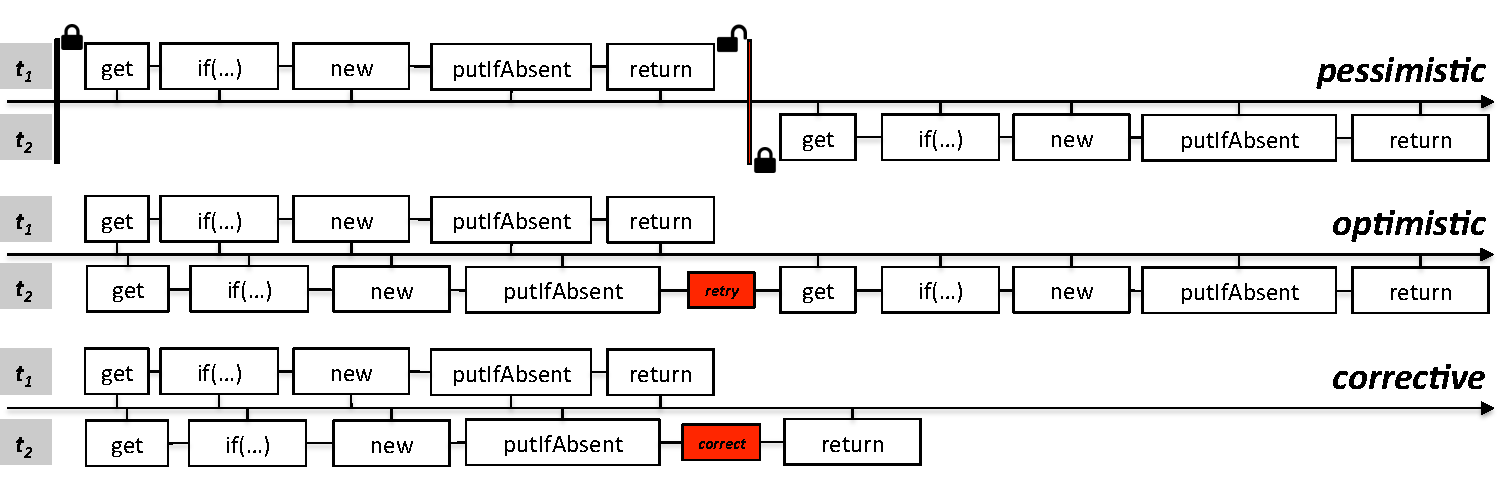
\includegraphics[width=\textwidth]{OverviewSlide.pdf}
	\end{center}
	\caption{\label{Fi:motivatingOverview}Interleaved execution of two instances of \textsf{getConvertors} using pessimistic, optimistic, and corrective synchronization.}
\end{figure*}

Both optimistic and corrective synchronization, allowing the problematic chain of interleavings, reach a nonserializable state. Optimism resolves this by retrying the entire transaction executed by, say, thread $t_2$. This yields serial execution, similar to the pessimistic run, where $t_2$ runs after $t_1$. Corrective synchronization, instead, ``fixes'' the final state, allowing $t_2$ to complete without rerunning any or all of its code.

We refer to corrective synchronization as \emph{sound} if $h'$ is the prefix of a serializable execution of the system. We refer to corrective synchronization as \emph{complete} if for any $h$, all the $h'$s that satisfy the conditions above are in the relation. In the following, we describe our method of computing a sound yet incomplete set of corrective targets via static analysis of the concurrent library.

A solution that is not complete faces the possibility of stuck runs: Given a (potentially) nonserializable execution prefix, the system does not have a corresponding serializable prefix to transition to. In this paper, we do not present a solution to the completeness problem, which we leave as future work. In the meantime, there are two simple strategies to tackle this problem: (i) \emph{manual specification}, whereby the user completes the set of corrective targets to ensure that there are no stuck runs (in our implementation, the targets are computed offline via static analysis, letting the user complete the specification ahead of deployment); and (ii) \emph{complementary techniques}, such as optimism, which the system can default to in the absence of a corrective target.
%\begin{compactitem}
%	\item Manual specification: The user completes the set of corrective targets computed automatically, such that there are no stuck runs. In our implementation of corrective synchronization, the corrective targets are computed offline via static analysis, which lets the user complete the specification prior to the deployment runs.
%	\item Complementary techniques: In the absence of a corrective target, the system can default to another synchronization technique such as STM. This provides a general means to avoid stuck states without causing any overhead w.r.t. standard techniques.
%\end{compactitem}


\smartpar{Computing Corrective Targets}
%
A simpler and more abstract specification to work with, compared to complete execution prefixes, is triplets $(s,s',s'')$ of states, such that there exist prefixes $h$ and $h'$ as above with respective initial and current states $(s,s')$ and $(s,s'')$, respectively. This form of specification is advantageous, because the corresponding runtime instrumentation is minimal compared to tracking the entire execution history. At the same time, however, merely recording initial and current states at runtime does not point back to prefixes $h$ and $h'$.

Mapping back from pairs of states to prefixes requires an oracle. In our prototype system, the oracle is computed as a relational abstract interpretation solution over the program that is sound yet incomplete. Specifically, an underapproximation of the serializable intermediate (or final) states is computed as the fixpoint solution over an interprocedural control-flow graph (CFG) of the form: 
	$t_1 \rightarrow t^\star_{2 \ldots n} \rightarrow t_{n+1} \rightarrow t'_1 \rightarrow t'^\star_{2 \ldots n} \rightarrow t'_{n+1} \rightarrow \ldots$,
where $t$, $t'$, etc denote different transaction types (i.e., transactions executing different code), and $n$ is unbounded, simulating a nondeterministic loop. This representation simulates an unbounded number of instances of transactions that are executed sequentially.

We go into detail about this representation in Section \ref{sec:transactionsystemwarping}, but here note that (i) this representation reflects the effects of serial execution of the transactions, and so the corrective targets are guaranteed to be sound; (ii) the nondeterministic loop captures an unbounded number of transactions; and (iii) the first and last transactions of a given type are purposely disambiguated to boost the precision of static analysis over the simulated execution.
%
As an illustration of the third point, in our running example the first transaction ( $t_1$) is modeled precisely in inserting the key/value pair into the {\sf Map} object. Analogously, the last transaction ($t_{n+1}$) can be confirmed not to update the key/value mapping.

\smartpar{Runtime Synchronization} 
%
The runtime system has two main responsibilities. First, it must track whether an execution has reached a (potentially) bad state. Second, if such a state arises, then the runtime system must map the current state onto a state that shares the same initial state and is known, by the oracle, to have a serializable continuation. 
%
In our implementation, the first challenge is addressed via a coarse conflict-detection algorithm that tracks API-level read/write behaviors (at the level of {\sf Map} operations). If read/write or write/write conflicts arise, then corrective synchronization is triggered in response. 

\OmerAdded{The second challenge, of deciding the target ``good'' state for a given ``bad'' state, is tackled via a pruning algorithm. During execution, the system maintains (as shadow state) a set of good symbolic final states. As individual transactions complete, incompatible final states (i.e., states that cannot be reached via any of the computed corrective actions) are pruned out. The remaining states are all guaranteed to be admissible targets. The decision which state to transition to is based on a heuristic measure of the cost of the corrective action (which simply counts the number of basic operations needed).}

We expand on both of these challenges in Section \ref{Se:system} and provide encouraging experimental results on a simple prototype in Section~\ref{Se:experiments}. Prior to that, in Sections \ref{se:instance} and \ref{sec:transactionsystemwarping}, we provide a formal statement of corrective synchronization.


\OmerAdded{
\subsection{Discussion}
As outlined above, the concrete instance that we have developed of corrective synchronization is specific to loop parallelization (in that transactions begin at the same time) and map clients. This particular setup is already applicable to many real-world codes \cite{oopsla/ShachamBASVY11,issta/ShachamYGABSV14}. Still, we emphasize that there are various natural extensions that widen this scope significantly and we intend to explore in the future.
}

%\OmerAdded{
%	First, there is no need, in general, to focus on maps. Concrete-level transactional memory ranges over variable and field accesses, enabling computation of corrective targets in terms of nonconflicting accesses to shared fields. For this any sound abstraction of runtime objects (e.g. as allocation sites) would suffice.
%}

\OmerAdded{A first extension is to consider additional ADTs, beyond map, such as set and counter \cite{ppopp08}. Assuming encapsulation \cite{TYFS:OOPSLA11}, it becomes possible to compose handling of different ADTs both with each other and with concrete-level corrective synchronization.}

\OmerAdded{The assumption regarding starting times can also be relaxed, albeit at the cost of more expensive offline analysis. While no change is needed to the core analysis algorithm, there are more cases that should be accounted for, namely all (or at least some of) the possibilities for transaction $t$ to start when concurrent transaction $t’$ is at a control location in its CFG other than the entry location. In our experimental results, the core analysis algorithm took less then a second to converge. Therefore, it can easily scale up to support thousands of combinations converging in at most one hour.}
	


%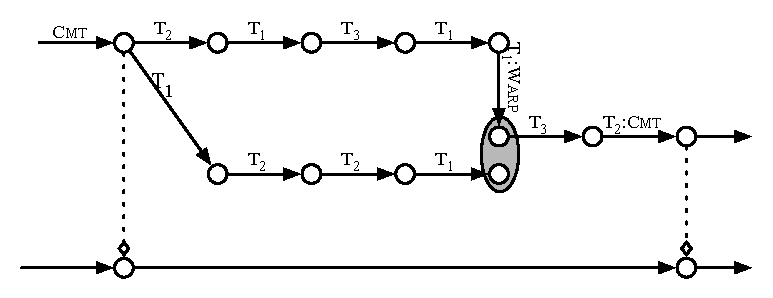
\includegraphics[width=3.2in]{simulation.eps}

%\newcommand\obseq{\stackrel{\sim}{=}}
\newcommand\CS{\{c,\sigma\}}
\newcommand\CpSp{\{c',\sigma'\}}
\newcommand\numCS[1]{\{c_{#1},\sigma_{#1}\}}


\begin{figure*}
\centering
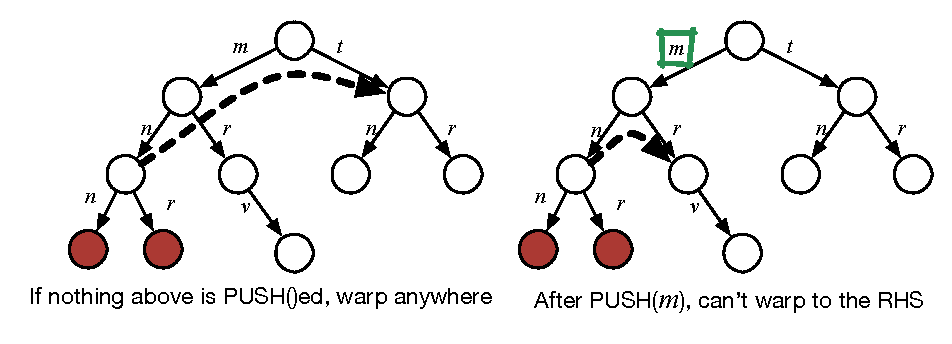
\includegraphics[width=5in]{stages.eps}
\caption{\red{caption.}}
\end{figure*}

\section{Technical Background}

In this section we describe a generic language of transactions and
define an idealized semantics for concurrent transactions called the
atomic semantics, in which there are no interleaved effects on the
shared state. 
%
The model preliminaries generalize those provided previously~\cite{PMPY}.
%
We also define a notion of \emph{good} configurations
and in the next section we will define how one can warp from a 
configuraiton that is not good to one that is.

\paragraph{Operations and States.}
We assume a set $M$ of method calls or operations (\eg\
  \texttt{ht.put('a',5)}).
%
State is represented in terms of
logs of operation records. An operation record (or, simply, an ``operation'')
$
    \op = \langle \opname, \lstack_1, \lstack_2, \opid \rangle
$
is a tuple consisting of the operation name $m$, 
a thread-local pre-stack $\lstack_1$ (method arguments),
a thread-local post-stack $\lstack_2$ (method return values),
and a unique identifier $\opid$.
%
We assume a predicate $\fresh{\opid}$ that holds provided that $\opid$
is globally unique (details omitted for lack of space).
%
In the atomic semantics defined below, the shared state $\OPL :
\textsf{list } \op$ is an ordered list of operations.
%
We use notations such as $\OPL_1\cdot\OPL_2$ and $\OPL\cdot \op$ to
mean append and appending a singleton, resp.

%\begin{parameter}[From logs to states: $\allowedt{}$] 
We require a prefix-closed predicate on operation lists $\allowed{\OPL}$
that indicates whether an operation log $\OPL$ corresponds to a state.
% The sequential specification
%   is a predicate on operation lists: $\allowed{\OPL}$. We require that it
%   be prefix closed.
%\end{parameter}
%
%\noindent
For convenience we will also write $\OPL \allows \langle m, \lstack_1,
\lstack_2, \opid\rangle$ which simply means 
$\allowed{\OPL \cdot \langle m, \lstack_1,\lstack_2, \opid\rangle}$.
%
For example, if we have a simple TM
based on memory read/write operations we expect
$\;\;\allowed{\OPL\cdot \langle \texttt{a := x}, [x \mapsto 5], [x
  \mapsto 5, a \mapsto 5], \opid\rangle}$,
but 
$\;\;\neg \allowed{\OPL\cdot \langle \texttt{a := x}, [x \mapsto 5], [x
  \mapsto 5, a \mapsto 3], \opid\rangle}$ or more elaborate
specifications that involve multiple tasks.
%
Ultimately, we expect the $\allowed{}$ predicate to be induced by the
implementation's operations on the state, $\llbracket op\rrbracket :
\mathcal{P}(\mathsf{State} \times \mathsf{State})$, and initial
states $I$. 
% If we give a denotation to logs as $\llbracket \OPL \cdot op
% \rrbracket \equiv \llbracket \OPL \rrbracket ; \llbracket op
% \rrbracket$, and $\llbracket \epsilon \rrbracket \equiv I$ , where $
% S ; R \equiv \{ s' \mid \exists s \in S. (s,s') \in R \}$. Then we
% can define $\allowed{\OPL}$ simply by checking if the denotation is
% non-empty, $(\llbracket \OPL \rrbracket \neq \emptyset)$.

%\paragraph{Operational equivalence.}
We define a precongruence over operation logs $\OPL_1 \opeq \OPL_2$
coinductively, by requiring that all \allowedt\ extensions of the log $\OPL_1$, are also \allowedt\ extension to the log $\OPL_2$. 
% This definition will ultimately be used in the simulation between
% \PMPY{} and an atomic machine.
We use a coinductive definition so that the precongruence can be
defined up to all infinite suffixes.
%\begin{definition}[Shared log precongruence $\opeq$] For all $\OPL_1, \OPL_2$,
$$
\infer={\OPL_1 \opeq \OPL_2} 
%   {\deduce{\allowed{\OPL_1}}  {\allowed{\OPL_2}}
   {  \allowed{\OPL_1} \Rightarrow \allowed{\OPL_2}
     & \forall \op.\   (\OPL_1 \cdot \op) \opeq (\OPL_2 \cdot \op)}
$$
We use a double-line here to indicate greatest fixpoint.
%\end{definition}
%
Informally, the above definition says that 
there is no sequence of observations we can make of $\OPL_2$, that we can't also make of $\OPL_1$. 
This is more general than just considering the set of states reached from executing the first log is included in the second:
unobservable state differences are also permitted. 


\paragraph{Language.}

Threads execute code $c$ from some programming language that
includes thread forking, transactions $\tx{c}$,
method names such as $m$, and a \skipt\ statement. As done
elsewhere~\cite{pmpy}, we abstract away the programming
  language with a few semantic functions: \red{update this with pldi
    camera ready}
%
\begin{description}
\item[$\step{c}{m}{c'}$:] Within a transaction, code $c$ can be reduced to the pair
  $(m,c')$.  That is, $m$ is a next reachable method call in the
  reduction of $c$, with remaining code $c'$.

\item[$\tstep{c}{t}{c'}$:] Outside of a transaction, code $c$ can be reduced to the pair
  $(t,c')$.  Here $c'$ is the remaining code, and $t$ is either
  a local state update, or a transaction or a thread fork.

\item[$\nothing{c}$:] This predicate is true provided that there is a
  reduction of $c$ to $\skipt$ that does not encounter a method call.
\end{description}
%
These functions allow us to obtain a simple semantics, despite an
expressive input language, by introducing functions to resolve
nondeterminism between method operation names and at the end of a
transaction.
%  As an example, one might use the generic language:
% \[ \begin{array}{rcl}
%   c &::=& c_1\plust c_2 \MOR c_1 \semit c_2
%       \MOR (c)^* \MOR \skipt \MOR \tx{c} \MOR \opname
% \end{array} \]
% %
% which consists of nondeterministic choice, sequential
% composition, and nondeterministic looping.
%
We assume that code is well-formed in that a single operation name $\opname$ 
is always contained within a transaction. 


The atomic semantics $\xrightarrow{a}$,
in which transactions are executed instantly, without interruption
from concurrent threads is given in Appendix~\ref{apx:atomic}.
Threads in the atomic semantics are represented as a pair
$(c,\sigma)$ of the code $c$ and a small amount of local
information $\sigma$ used to model arguments and return values.


%%% Local Variables:
%%% mode: latex
%%% TeX-master: "paper"
%%% End:


%\newcommand\STEP{{\sc step}}
\newcommand\BEGIN{{\sc begin}}
\newcommand\LOCAL{{\sc local}}
\newcommand\FIN{{\sc fin}}
\newcommand\FORK{{\sc fork}}

\subsection{The \PUSH{}/\PULL{} model}

We briefly summarize the \PUSH{}/\PULL{} model~\cite{KoskinenP15}. This model consists of
seven rules which we will use for both intuitive descriptions of the
Warping protocol, and in the formal proof of serializability.
The \PMPY{} model involves rule that characterize how a given transaction moves forward/backward
locally, how it may share its effects into the shared view (\PUSH),
and bring the effects of other transactions into its local view
(\PULL). 
The  model is a log-based transition relation
$\Ts,G \pmpyreduce \Ts', G'$ that reduces
a list of threads $\Ts : \textsf{list } (c\times \lstack
\times L)$ and a global log $G$ to $\Ts',G'$.
%
There is a per-thread local log $L$ and a global log $G$.
The rules are:
\begin{itemize}
\item \APPLY: A thread reduces its (nondeterminisitc) code down to a
  next-reachable operation $\op$ (with continuation code). This
  operation $\op$ is applied to the local log but is not yet shared
  into the global log. It is yet ``unpushed.''

\item \UNAPP: This rule undoes the most recent \APPLY, restoring the
  previous code and local state, and discarding the most recent
  operation from the local log.

\item \PUSH: A transaction shares its effects with the global view by
  copying an $\op$ from its local log and appending it to the global
  log. Locally, $\op$ is considered ``pushed'' and, in the global log,
  it is marked as ``uncommitted.''
%
  This rule can only be taken if all uncommitted operations in the
  shared log can commute with (move to the right of) $\op$.
%
  Moreover, it is possible to \PUSH{} operations to the shared log in
  a different order than they appear in the local log (provided that
  each pushed $\op$ commutes with its earlier unpushed neighbors in the local log).

\item \UNPUSH: An operation $\op$ that has been \PUSH{}ed to the
  shared log can be \UNPUSH{}ed by swapping the flag from ``pushed''
  to ``unpushed'' and removing the corresponding global log entry for
  $\op$. $\op$ can only be \UNPUSH{}ed if it commutes with the
  subsequently pushed operations in the log.

\item \PULL:
%
  Transactions can learn about the published effects of other
  transactions by \PULL{}ing operations from the global log into their
  local logs. Provided it has not alreadty been pulled, an operation
  $\op$ can be copied from the global log, appended to the local log,
  and marked as ``pulled.'' A transaction does not need to \PULL{} in
  shared-log-chronological order.

\item \UNPULL: (description omitted for lack of space)

\item \CMT: \red{todo}
%  and local state manipulations (\LOCAL
\end{itemize}
%The full descriptions of these rules are given in Appendix~\ref{apx:bigfig}.
Note that each of the above rules (except for \CMT) have an opposite rule.
%
Other rules include transaction initiation (\BEGIN),
thread completion (\FIN) and forking (\FORK).
As shown previously~\cite{KP:PLDI15}, each rule comes with a few
criteria which, all told, ensure serializability and---when
appropriately restricted---opacity.




%%% Local Variables:
%%% mode: latex
%%% TeX-master: "paper"
%%% End:


%

\section{Warping}
\label{sect:warping}

The key idea of this paper is that when transactions run
awry into an inconsistent state, rather than aborting them and
starting again from the beginning, it may be possible to
\emph{correct} the shared/local state directly by directly
modifying the state. Thus, the program continues as if it had not
gone down the bad path to the inconsistent state.
In this way we exploit a large design space, predicted by the \PMPY{}
model, but yet unexplored.

A thread $(c\times \lstack \times L)$ consists of code $c$, some local
stack $\lstack$ (for arguments and return values), and a local log
$L$. When executing a transaction, the code is of the form $\tx{c}$.
%
A given code $c$ induces a tree, with the root node labeled $c$. For
each $m$ and $c'$ such that $\step{c}{m}{c'}$, we create a child node
labled $c'$ and label the arc as $m$. If, for a node labeled $c$,
$\nothing{c}$ holds, then that note shall be a leaf.  We will
illustrate warping with the following example tree:
\begin{center}
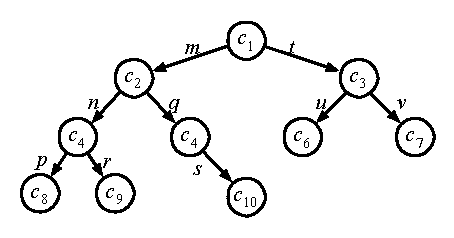
\includegraphics[width=2.8in]{stages0.eps}
\end{center}

\paragraph{Warping.}
The main idea of corrective synchronization is that transactions, in
instances of conflict, change their behavior to another possible
\red{more...}

Let us say, for example, that the example transaction has already
executed the following path:
\[\begin{array}{cl}
 (c_1,\lstack,[])\\
  \downarrow & \text{\APPLY}: \step{c_1}{m}{c_2} \text{ and } L'=L\cdot[m]\\
 (c_2,\lstack',[m])\\
  \downarrow & \text{\APPLY}: \step{c_2}{n}{c_4} \text{ and } L'=L\cdot[n]\\
 (c_4,\lstack'',[m,n])\\
\end{array}\]
% \begin{itemize*}
% \item From $(c_1,\lstack,[])$, $\step{c_1}{m}{c_2}$ holds, so \APPLY{}$(m)$.
% \item From $(c_2,\lstack',[m])$, $\step{c_2}{n}{c_4}$ holds, so \APPLY{}$(n)$.
% \item Ending at $(c_4,\lstack'',[m,n])$
% \end{itemize*}
For now, let us assume for simplicity that the transaction has not
\PUSH{}ed any of these methods.

At this stage, let us say that another transaction has committed. This
event may introduce conflict, either with one of the methods already
performed ($m$ or $n$) or with some/all of the methods in the subtree
of $c_4$: $p$ and $r$. When conflict is inevitable, standard
transactional memory implementations have no choice but to abort the
transaction and roll back to the original code $c_1$.

We observe that, in some cases, it may be more efficient to avoid the
process of aborting and restarting and instead, \emph{correcting}
behavior by transitioning directly to an alternate location on the
transaction tree, where the outlook is better. Consider this diagram:
\begin{center}
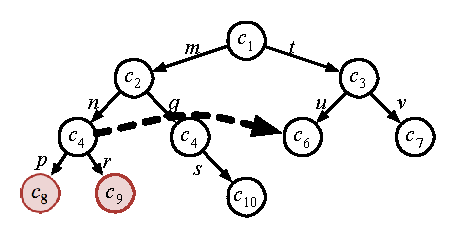
\includegraphics[width=2.8in]{stages1.eps}
\end{center}
Here the transaction has 

\paragraph{Correction.}

code\\
local state\\
log correction of $[n^{-1};m^{-1};t;u]$

\paragraph{Adding pessimistic behavior.}
%
The description thus far has been purely optimistic: a transaction
does not share its effects until it commits. A transaction may
\PUSH{} some of its effects to the shared log. However, this
constrains the transaction's warp destinations. 
%
If, in the running example, operation $m$ has been \PUSH{}ed, then it
is not possible for the transaction to warp to any node in the right
subtree of $c_1$. The transaction may, however, warp to node $c_4$,
applying a correction of $[n^{-1};q]$.
%
It is only possible for the transaction to warp to the right subtree
of $c_1$ if it first rolls backward, \UNPUSH{}ing $m$. This may
require global coordination if another transaction has already \PULL{}ed $m$.

\begin{theorem} The transition system is serializable.
\begin{proof}Via simulation with the \PMPY{} model~\cite{KP:PLDI15}.
\end{proof}
\end{theorem}

Being able to perform these warp operations depends crucially on a
few factors that we will explore in the rest of this paper:
\begin{itemize*}
\item Detecting when conflict is inevitable.
\item Detecting which warp destinations are possible and conflict-free.
\item How to correct: modifing the current local state, stack and
  program counter so that it
  is compatible with that alternate destination
\end{itemize*}
We address these issues with a combination of static and dynamic analysis.

\red{what about side effects?}

%%% Local Variables: 
%%% mode: latex
%%% TeX-master: "paper"
%%% End: 



\newcommand{\pengtodo}[1]{{\bf #1}}
\newcommand{\pietrotodo}[1]{{\bf #1}}


\section{Transaction Semantics}
\label{sec:concretesemantics}
\subsection{Notation}

In our description of the transition system, we utilize the following semantic domains:
\\
\begin{tabular}{rcll}
	\\
	$T \subset {\cal T}$ & $:=$ & transaction IDs \\
	$c \in {\cal C}$ & $:=$ & command \\
	$\sigma \in \Sigma$ & $:=$ & shared state \\
	${\sigma_t}$ & $:=$ & local state of $t$ \\
	$L \in {\cal L}$ & $:=$ & shared log \\
	$L_t$ & $:=$ & local log of $t$ \\
	$s = (T, [t \mapsto (c_t,\sigma_t,L_t)]_{t \in T}, \sigma, L) \in {\cal S}$ & $:=$ & system state \\
	\\
\end{tabular}
\\
We assume that the set $\Sigma$ of shared states is closed under composition, denoted $\cdot$. That is,
$\forall \sigma,\sigma' \in \Sigma.\ \sigma \cdot \sigma' \in \Sigma$. Hence, we can decompose a given shared state into (disjoint) substates (the standard decomposition being into memory locations), such that we can easily refer to the read/write effects of a given operation.

We additionally define two helper functions:
\begin{itemize}
\item $w \colon\ {\cal C} \times {\cal S} \rightharpoonup \Sigma$: the portion of the shared state written by a given atomic operation
\item $r \colon\ {\cal C} \times {\cal S} \rightharpoonup \Sigma$: the portion of the shared state read by a given atomic operation
\end{itemize}
The notation $\rightharpoonup$ denotes that $w$ and $r$ are partial functions. The shared log $L$ consists of pairs $\left\langle t,o \right\rangle$, where $t$ is a transaction identifier and $w(c) \neq \bot$.

\subsection{Transition System}

We define four transactional events, as follows:
\begin{itemize}
\item The {\sf bgn} event marks the beginning of a transaction.
\item The {\sf cmt} event fires when a transaction publishes its outstanding log of operations that affect the shared state to the shared state and log.
\item The {\sf end} event marks the termination of a transaction.
\item The {\sf warp} event enables a transaction to modify its local state and log, under certain restrictions, as a means to recover from potentially inadmissible thread interleavings.
\end{itemize}
We define the semantics of these events in the following. For rules where a transaction $t$ is defined in the prestate, its corresponding local configuration is denoted $(c_t,\sigma_t,L_t)$. We utilize helper function ${\sf serpref} \colon\ {\cal L} \rightarrow \{ {\sf true},{\sf false} \}$ to (conservatively) determine whether a given shared log is the prefix of some serializable execution log. Finally, we define helper function
${\sf ref} \colon\ {\cal T} \rightarrow {\cal S}$ that --- given a transaction $t$ --- retrieves the (global) system state immediately preceding $t$'s start.

The events are defined as follows:
\\
\begin{tabular}{rc}
\\
{\sf bgn}\ $t,c$ & $\infer{(T, \mu, \sigma, L) \rightarrow (T \cup \{ t \}, \mu \cdot [t \mapsto (c,\bot,\epsilon)], \sigma, L)}{t \notin T}$ \\
\\
{\sf cmt}\ $t$ & $\infer{(T, \mu, \sigma, L) \rightarrow (T, \mu[t \mapsto (c_t,\sigma_t,\epsilon)], \llbracket L_t \rrbracket(\sigma), L \cdot L_t)}{t \in T, L_t \neq \epsilon, {\textnormal{\sf serpref}\ L \cdot L_t}}$ \\
\\
{\sf end}\ $t$ & $\infer{(T, \mu, \sigma, L) \rightarrow (T \setminus \{ t \}, \mu \setminus [t \mapsto \mu(t)], \sigma, L)}{t \in T, \mu(t) = ({\sf skip}, \_, \epsilon)}$ \\
\\
{\sf warp}\ $t$ & $\infer{(T, \mu, \sigma, L) \rightarrow (T,\mu[t \mapsto \mu'(t)], \sigma, L)}{
	t \in T, 
	{\sf ref}\ t \leadsto (T,\mu', \sigma, L)}$\\
\\
{\sf local}\ $t$ & $\infer{(T, \mu, \sigma, L) \rightarrow (T,\mu[t \mapsto (c'_t,\sigma'_t,L_t)], \sigma, L)}
{t \in T, (c_t,\sigma_t) \rightarrow (c'_t,\sigma'_t)}$\\
\\
\end{tabular}
\\
Note that the {\sf warp} rule only applies changes to the local configuration corresponding to the given transaction $t$. All other transactions retain their original local configurations.

\subsection{Formal Guarantees}

\begin{theorem}[Soundness] Any terminating execution of the transition system is guaranteed to yield a serializable shared log.
\begin{proof}
	The {\sf cmt} event acts as a gatekeeper, demanding that the log prefix including the outstanding events about to be committed is serializable. The check executes atomically together with the log update. Hence the system is guaranteed to terminate with a serializable shared log.	
\end{proof}
\end{theorem}

\begin{definition}[Progress]
	We say that the transition system has made progress, transitioning from (global) state $s$ to (global) state $s'$, if the associated event $e$ for
	$s \stackrel{e}{\longrightarrow} s'$ is either a ${\sf cmt}$ event or an ${\sf end}$ event.
\end{definition}

\begin{definition}[Progress-safe warping]
	Let ${\sf warp}\ t$ occur at system state $s=(T,\mu,\sigma,L)$, such that state $s'=(T,\mu[t \mapsto (c_t,\sigma_t,L_t)],\sigma,L)$ is reached. Assume that there is a reduction
	$(\sigma_t,c_t,L_t) {\longrightarrow} (\sigma'_t,c'_t,L'_t)$, such that 
	at system state $s''=(T,\mu[t \mapsto (\sigma'_t,c'_t,L'_t)],\sigma,L)$ either (i)  ${\sf cmt}\ t$ is enabled or (ii) ${\sf end}\ t$ is enabled. Then we refer to ${\sf warp}\ t$ at $s$ with target $(\sigma_t,c_t,L_t)$ as \emph{progress safe}.
\end{definition}

Note that from the perspective of transaction $t$, the local states of other transactions are irrelevant to whether a commit (or end) transition is enabled for $t$. The only cause of a failed commit is if other threads have committed. We can therefore relax the definition above to refer to any system state $s''=(T',\mu',\sigma,L)$, such that $t \in T'$ and 
$[t \mapsto  (\sigma'_t,c'_t,L'_t)] \in \mu'$.

\begin{example}[Self warping]\label{Ex:selfwarp}
	Given transaction $t$ with local state $(\sigma_t,c_t,L_t)$, we refer to target
	$(\sigma'_t,c_t,L'_t)$ as a \emph{self-warping target}. Post warping, the transaction has the same command left to reduce, but its state and outstanding log of operations are modified. A specific instance is $(\sigma_t,{\sf skip},L_t) \rightarrow (\sigma'_t,{\sf skip},L'_t)$. This pattern of warping is progress safe if commits are attempted at join points, which enables simulation of alternative control-flow paths (and therefore also logged effects) via warping.
\end{example}

\begin{theorem}[Progress]\label{Th:progress} Assume that (i) a ${\sf warp}\ t$ event only fires when a transaction $t$ reaches a commit point but fails to commit, and (ii) warping instances are progress safe. Then progress is guaranteed.
	\begin{proof}
	Given system state $s$, if there exists a transaction $t$ that is able to either commit or complete then the proof is done. Otherwise, there is a transaction $t$ that reaches a commit point at some state $s'$ and fails. At this point, ${\sf warp}\ t$ is the only enabled transition for $t$, and by assumption (ii), the warping instance is progress safe. At this point, there are two possibilities. Either $t$ proceeds without other threads modifying the shared state, such that a commit or completion point is reached by $t$ (without warping prior to reaching such a point according to assumption (i)), in which case progress has been achieved, or one or more threads interfere with $t$ by committing their effects, in which case too progress has been achieved.
	\end{proof}
\end{theorem}

\begin{definition}[Complete warping] 
	We say that the system is complete w.r.t. warping if for any state $s$, if a ${\sf warp}\ t$ transition is executed in $s$, then the selected warping target satisfies progress safety.
\end{definition}

\begin{lemma}[Termination]
	Assume that the system performs warping only on failed commits, and is complete w.r.t. warping. Further assume that throughout any run of the system, only boundedly many transactions are created (via a {\sf bgn} event), and these transactions do not have infinite executions. Then termination is guaranteed.
	\begin{proof}
		The first two assumptions guarantee progress, as established above in 
		Theorem \ref{Th:progress}. Since transactions are finite, each transactions may perform finitely many {\sf cmt} transitions before terminating via an {\sf end} transition. This implies that after finitely many transitions, some transaction $t$ will terminate. This argument applies to the resulting system until no transactions are left.
	\end{proof}
\end{lemma}

\begin{example}[Loop parallelization]\label{Ex:loops}
	Assume the common case of loop parallelization, where loop iterations are executed in parallel as transactions. There are normally finitely many transactions, all starting at the same time, and all are expected to terminate within a finite number of steps. Complete on-commit-failure warping guarantees both termination and serializability in this setting.
\end{example}

%\subsection{Other Stuff}
%
%Events might be {\tt start}, {\tt read}, {\tt write}, {\tt warp}, {\tt commit}, {\tt abort}, and {\tt end}. Figure \ref{fi:semantics} formalizes the concrete semantics, where $a.b$ denotes the concatenation of sequence $a$ and sequence $b$, and $p_t$ represents the sequence of actions transaction $t$ performs.
%
%\begin{figure*}

%\begin{center}
%\begin{tabular}{c}
%\\
%$\infer{\langle t, {\tt start}, (sh, tl, g, l)\rangle \to (sh, tl[t \mapsto (p_t, sh)], g, l[t \mapsto \epsilon])}{}$\\
%\\
%$\infer{\langle t, {\tt read}, (sh, tl, g, l)\rangle \to (sh, tl, g, l[t \mapsto l(t).{\tt read}])}{}$\\
%\\
%$\infer{\langle t, {\tt write}, (sh, tl, g, l)\rangle \to (sh, tl[t \mapsto \llbracket {\tt write}\rrbracket](tl(t)), g, l[t \mapsto l(t).{\tt write}])}{}$\\
%\\
%$\infer{\langle t, {\tt commit}, (sh, tl, g, l)\rangle \to (\llbracket l(t) \rrbracket(sh), tl, g.l(t), l\setminus [t \mapsto l(t)])}
%{\textrm{if there is no conflict}}$\\
%\\
%$\infer{\langle t, {\tt commit}, (sh, tl, g, l)\rangle \to \langle t, {\tt warp}, (sh, tl, g, l)\rangle}
%{\textrm{if there is a conflict}}$\\
%\\
%$\infer{\langle t, {\tt warp}, (sh, tl, g, l)\rangle \to (sh, tl[t \mapsto s], g, l[t \mapsto i])}
%{\textrm{if the warping system produces state } s \textrm{ and  log } i}$\\
%\\
%$\infer{\langle t, {\tt end}, (sh, tl, g, l)\rangle \to (\llbracket l(t) \rrbracket(sh), tl \setminus [t \mapsto tl(t)], g.l(t), l\setminus [t \mapsto l(t)])}
%{}$\\
%\end{tabular}
%\caption{Concrete semantics}
%\label{fi:semantics}
%\end{center}
%\end{figure*}

%
%\section{Language}
\label{sect:language}

\begin{figure}[t]
	\begin{center}
		\begin{tabular}{l}
			\statement{s ::= m.put(k, v)}\\
			\hspace{15pt} \statement{|\ v=m.get(k)}\\
			\hspace{15pt} \statement{|\ m.remove(k)}\\
			\hspace{15pt} \statement{|\ v=m.putIfAbsent(k, v)}\\
			\hspace{15pt} \statement{|\ v=new\ Value()}\\
			\hspace{15pt} \statement{|\ v=null}\\
			\hspace{15pt} \statement{|\ assert(b)}\\
%			\hspace{15pt} \statement{|\ if(b)\ s_1;\ else\ s_2}\\
%			\hspace{15pt} \statement{|\ while(b)\ s_1;}\\
%			\hspace{15pt} \statement{|\ s_1;\ s_2}\\
			\\
			\statement{b ::= x==NULL\ |\  x!=NULL}\\
			\hspace{15pt} \statement{|\ m.containsKey(k)\ |\ ! m.containsKey(k)}\\
		\end{tabular}
	\end{center}
	\caption{Statements and conditions}
	\label{fig:language}
\end{figure}


As a proof of concept and preliminary practical study, we instantiate the theoretical framework we formalized in the Section \ref{sect:warping} on the language in Figure \ref{fig:language}, developing a static analysis to compute warping \pietrotodo{targets}, and a dynamic system to warp.

The language is focused on a representative set  of operations of the Java \statement{Map} interface. In Figure \ref{fig:language}, we represent by \statement{m} the map shared among all the transactions, and \statement{k} the shared key. The values inserted or read from the map might be a parameter of the transaction, or created through a \statement{new} statement. Following the semantics of the Java library, our language supports (i) \statement{v=m.get(k)} that returns the value \statement{v} related with key \statement{k}, or \statement{null} if \statement{k} is not in the map, (ii) \statement{m.remove(k)} removes \statement{k} from the map, (iii) \statement{v=m.putIfAbsent(k, v)} relates \statement{k} to \statement{v} in \statement{m} if \statement{k} is already in \statement{m} and returns the previous value it was related to, (iv) \statement{v=new\ Value(...)} creates a new value, and (v) \statement{v=null} assigns \statement{null} to variable \statement{v}. In addition, our language support standard \statement{if} and \statement{while} statements, as well as concatenation of statements.

As Boolean conditions, the language supports checking if a variable is \statement{null}, and if the map contains a key.

\subsection{Running Example}

\begin{figure}
\begin{lstlisting}
Value removeAttribute(Key k) {
  Value result = null;
  if(map.containsKey(k)) {
    result = m.get(k);
    m.remove(k);
  }
  return result;
}

boolean removeAttribute(Key k, Value v) {
  Value oldvalue = m.get(k);
  m.put(k, v);
  return oldvalue != null;
}
\end{lstlisting}
\caption{The running example inspired by class \statement{ApplicationContext} of Apache Tomcat}
\label{lst:runningexamplestaticanalysis}
\end{figure}

Figure \ref{lst:runningexamplestaticanalysis} illustrates our running example. This code is inspired by \pietrotodo{XXX}. The first type of transaction (\statement{transaction1}) removes the value associated with the given key \statement{k}, and returns it. Instead, the second type of transaction relates \statement{k} with a given value \statement{v}, and returns \statement{true} if the key was already in the map. During the formalization of the static analysis and the warping system, we will refer to this running example where each transaction is instantiated multiple times, and all transactions conflict on the same key \statement{k}.

\newcommand{\set}[1]{\mathsf{#1}}
\newcommand{\isSummary}{\set{isSummary}}
\newcommand{\freshNode}{\set{fresh}}
\newcommand{\heapnode}{\set{HeapNode}}
\newcommand{\reference}{\set{Ref}}
\newcommand{\variable}{\set{Var}}
\newcommand{\env}{\set{Env}}
\newcommand{\map}{\set{Map}}
\newcommand{\aset}[1]{\set{#1}}
\newcommand{\state}{\set{\Sigma}}
\newcommand{\aenv}{\aset{Env}}
\newcommand{\amap}{\aset{Map}}
\newcommand{\astate}{\aset{\Sigma}}
\newcommand{\multistate}{\set{\Phi}}
\newcommand{\amultistate}{\aset{\multistate}}
\newcommand{\serializedCFGs}{\set{serializedCFGs}}
\newcommand{\isconcrete}{\set{single}}
\newcommand{\warpdestination}{\set{corrTarg}}
\newcommand{\concretetransactions}{{\cal T}}
\newcommand{\abstracttransactions}{\concretetransactions^\#}

\section{Thread Local Semantics}
\label{se:instance}
We now instantiate the theoretical framework introduced in Section \ref{sec:concretesemantics} to a language supporting some standard operations on concurrent shared maps. In this Section, we define the thread-local concrete semantics of this language instantiating $\semanticanome{C}$ of the {\sf local} rule introduced in Section \ref{sec:transitionsystem}. Following the abstract interpretation theory, we then introduce an abstract domain and semantics that computes an approximation of the concrete semantics. This thread-local abstract semantics will be used in Section \ref{sec:transactionsystemwarping} to compute progress-safe corrective targets.


\subsection{Language}
\label{sect:language}

%\begin{figure}[t]
%	\begin{center}
%		\footnotesize
%		\begin{tabular}{l}
%			\statement{s ::= m.put(k, v)} \statement{|\ v=m.get(k)}\\
%			\hspace{15pt} \statement{|\ m.remove(k)} \statement{|\ v=m.putIfAbsent(k, v)}\\
%			\hspace{15pt} \statement{|\ v=new\ Value()} \statement{|\ v=null} \statement{|\ assert(b)}\\
%			%			\hspace{15pt} \statement{|\ if(b)\ s_1;\ else\ s_2}\\
%			%			\hspace{15pt} \statement{|\ while(b)\ s_1;}\\
%			%			\hspace{15pt} \statement{|\ s_1;\ s_2}\\
%			\statement{b ::= x\ ==\ null\ |\  x\ !=\ null}\\
%			\hspace{15pt} \statement{|\ m.containsKey(k)\ |\ ! m.containsKey(k)}
%		\end{tabular}
%	\end{center}
%	\caption{Fragment of the language}
%	\label{fig:language}
%\end{figure}
We focus our formalization on the following language fragment:
	\footnotesize\\\\
	\begin{tabular}{l}
		\statement{s ::= m.put(k, v)} \statement{|\ v=m.get(k)}
		\statement{|\ m.remove(k)} \statement{|\ v=null}\\
		\hspace{7.5pt} \statement{|\ v=m.putIfAbsent(k, v)} \statement{|\ v=new\ Value()}  \statement{|\ assert(b)}\\
		%			\hspace{15pt} \statement{|\ if(b)\ s_1;\ else\ s_2}\\
		%			\hspace{15pt} \statement{|\ while(b)\ s_1;}\\
		%			\hspace{15pt} \statement{|\ s_1;\ s_2}\\
		\statement{b ::= x==null\ |\  x!=null}
		\statement{|\ m.containsKey(k)\ |\ ! m.containsKey(k)}
	\end{tabular}
	\\\\
	\normalsize
This fragment captures a representative set of operations of the Java 7 \statement{java.util.concurrent.ConcurrentMap} class.\footnote{\url{http://docs.oracle.com/javase/7/docs/api/java/util/concurrent/ConcurrentMap.html}} We represent by \statement{m} the map shared among all the transactions, and \statement{k} a shared key. The values inserted or read from the map might be a parameter of the transaction, or created through a \statement{new} statement. Following the semantics of the Java library, our language supports (i) \statement{v=m.get(k)} that returns the value \statement{v} related with key \statement{k}, or \statement{null} if \statement{k} is not in the map, (ii) \statement{m.remove(k)} removes \statement{k} from the map, (iii) \statement{v=m.putIfAbsent(k, v)} relates \statement{k} to \statement{v} in \statement{m} if \statement{k} is already in \statement{m} and returns the previous value it was related to, (iv) \statement{v=new\ Value(...)} creates a new value, and (v) \statement{v=null} assigns \statement{null} to variable \statement{v}. In addition, our language supports a standard \statement{assert(b)} statement that let the execution go through iff the given Boolean condition holds. In particular, the language supports checking if a variable is \statement{null}, and if the map contains a key. This statement is necessary to support conditional and loop statements.


%\subsubsection{Running Example}
%
%\begin{figure}
%\begin{lstlisting}
%Value removeAttribute(Key k) {
%  Value result = null;
%  if(map.containsKey(k)) {
%    result = m.get(k);
%    m.remove(k);
%  }
%  return result;
%}
%	
%boolean removeAttribute(Key k, Value v) {
%  Value oldvalue = m.get(k);
%  m.put(k, v);
%  return oldvalue != null;
%}
%\end{lstlisting}
%\caption{The running example inspired by class \statement{ApplicationContext} of Apache Tomcat}
%\label{lst:runningexamplestaticanalysis}
%\end{figure}
%
%XXX Somewhere else? XXX
%
%In this Section, we will refer to the motivating example of Figure \ref{Fi:introMotivating}. 
%
%Figure \ref{lst:runningexamplestaticanalysis} illustrates our running example. This code is inspired by \pietrotodo{XXX}. The first type of transaction (\statement{transaction1}) removes the value associated with the given key \statement{k}, and returns it. Instead, the second type of transaction relates \statement{k} with a given value \statement{v}, and returns \statement{true} if the key was already in the map. During the formalization of the static analysis and the warping system, we will refer to this running example where each transaction is instantiated multiple times, and all transactions conflict on the same key \statement{k}.


\subsection{Concrete Domain and Semantics}
\label{sec:concretemap}
First of all, we instantiate the state of a transaction $t$ introduced in \ref{sec:concretedomain} to the language of Section \ref{sect:language}.

Let $\variable$ and $\reference$ be the set of variables and references, respectively. Keys and values are identified by concrete references, and we assume $\statement{null}$ is in $\reference$. We define by $\env : \variable \to \reference$ the environments relating local variables to references. A map is then represented as a function $\map : \reference \to \reference$, relating keys to values. The value $\statement{null}$ represents that the related key is not in the map. A single concrete state is a pair made by an environment and a map. Formally, $\state = \env \times \map$. As usual in abstract interpretation, we collect a set of states per program point. Therefore, our concrete domain is made by elements in $\wp(\state)$, and the lattice relies on standard set operators. Formally, $\langle \wp(\state), \subseteq, \cup \rangle$.



\begin{figure}
	\footnotesize
	\vspace{-5pt}
	\[
	\begin{array}{l}
	\csemantics{C}{\statement{m.put(k, v)}, (e, m)} = 
	(e, m[e(\statement{k}) \mapsto e(\statement{v})])\\
	\csemantics{C}{\statement{v=m.get(k)}, (e, m)} = (e[\statement{v} \mapsto m(e(\statement{k}))], m) \\
	\csemantics{C}{\statement{m.remove(k)}, (e, m)} = 
	(e, m[e(\statement{k}) \mapsto \statement{null}])\\
	\csemantics{C}{\statement{v = m.putIfAbsent(k, v)}, (e, m)} =  (e[\statement{v} \mapsto m(n)], m') : \\
	\hspace{70pt} 
	m'=
	\left\{
	\begin{array}{ll}
	m[n \mapsto e(\statement{v})]) & \textrm{ if } m(e(\statement{k})) = \statement{null}\\
	m & \textrm{ otherwise}\\
	\end{array}
	\right. \\
	\csemantics{C}{\statement{v = new\ Value()}, (e, m)} =  (e[v \mapsto \freshNode(\statement{t})], m)\\
	\csemantics{C}{\statement{v = null}, (e, m)} =  (e[v \mapsto \{\statement{null}\}], m)\\
	\csemantics{C}{\statement{assert(x==null)}, (e, m)} = (e,m) \textrm{ if } e(\statement{x})=\statement{null}\\
	\csemantics{C}{\statement{assert(x!=null)}, (e, m)} = (e,m ) \textrm{ if } e(\statement{x})\neq\statement{null}\\
	\csemantics{C}{\statement{assert(m.containsKey(k))}, (e, m)} = (e, m) \textrm{ if } m(e(\statement{k})) \neq \statement{null}\\
	\csemantics{C}{\statement{assert(!m.containsKey(k))}, (e, m)} =(e, m) \textrm{ if } m(e(\statement{k})) = \statement{null}\\
	\end{array}
	\]
	\caption{Concrete semantics}
	\vspace{-5pt}
	\label{fig:concretesemantics}
\end{figure}


Figure \ref{fig:concretesemantics} defines the concrete semantics. For the most part, the concrete semantics formalizes the API specification of the corresponding Java method. Note that \statement{assert} is defined only on the states that satisfy the given Boolean conditions. In this way, the concrete semantics filters out only the states that might execute a branch of an \statement{if} or \statement{while} statement.

\subsection{Abstract Domain}
\label{sect:abstractate}

Let $\heapnode$ be the set of abstract heap nodes with $\statement{null} \in \heapnode$. Both keys and values are abstracted as heap nodes. As usual with heap abstractions, each heap node might represent one or many concrete references. Therefore, we suppose that a function $\isSummary : \heapnode \to \{\true, \false\}$ is provided; $\isSummary(n)$ returns $\true$ if $n$ might represent many concrete nodes (that is, it is a summary node). We define by $\aenv : \variable \to \wp(\heapnode)$ the set of (abstract) environments relating each variable to the set of heap nodes it might point to. A map is represented as a function $\amap : \heapnode \to \wp(\heapnode)$, connecting each key to the set of possible values it might be related to in the map. The value $\statement{null}$ represents that the key is not in the map. For instance, $[n_1 \mapsto \{\statement{null}, n_2\}]$ represents that the key $n_1$ might not be in the map, or it is in the map, and it is related to value $n_2$. An abstract state is a pair made by an abstract environment and an abstract map. We augment this set with a special bottom value $\bot$ to will be used to represent that a statement is unreachable. Formally, $\astate = (\aenv \times \amap) \cup \{\bot\}$.

The lattice structure is obtained by the point-wise application of set operators to elements in the codomain of abstract environments and functions. Therefore, the abstract lattice is defined as $\langle \astate, \dot{\subseteq}, \dot{\cup} \rangle$, where $\dot{\subseteq}$ and$\dot{\cup}$ represents the point-wise application of set operators $\subseteq$ and $\cup$, respectively.

%For the sake of simplicity, we omit in the formalization the local log in the abstract domain. The only difference w.r.t. the concrete local log is that the entries refer to abstract heap nodes in $\heapnode$ instead of concrete references in $\reference$, and the presences of the entry \statement{?put} representing a possible \statement{put} action. This will be used in the definition of the abstract semantics of statement \statement{putIfAbsent}. XXX We can formalize the log. However, the problem is that the sequence might be infinite, so we need some kind of regular expressions - not sure I'm willing to go into this direction XXX 

\noindent \textbf{Running example.} 
Consider the motivating example in Figure \ref{Fi:introMotivating}. Abstract state $([\statement{name} \mapsto \{n_1\}], [n_1 \mapsto \{\statement{null}\}])$ represents that the key \statement{name} is not in the map, while $([\statement{name} \mapsto \{n_1\}], [n_1 \mapsto \{n_2\}])$ represents that it is in the map, and it is related to some value $n_2$. Finally, $([\statement{name} \mapsto \{n_1\}], [n_1 \mapsto \{\statement{null}, n_2\}])$ represents that \statement{name} (i) might not be in the map, \emph{or} (ii) is in the map related to value $n_2$.

\subsection{Concretization function.}
We define the concretization function $\gamma_\state : \astate \to \wp(\state)$ that, given an abstract state, returns the set of concrete states it represents. First of all, we assume that a function concretizing abstract heap nodes to concrete references is given. Formally, $\gamma_\reference : \heapnode \to \wp(\reference)$. We assume that this concretization function concretizes \statement{null} into itself ($\gamma_\reference(\statement{null})=\{\statement{null}\}$), and that it is coherent w.r.t. the information provided by $\isSummary$ ($\neg \isSummary(n) \Leftrightarrow |\gamma_\reference(n)|=1$).

The concretization of abstract environments relates each variable in the environment to a reference concretized from the node it is in relation with. Similarly, the concretization of abstract maps relates a reference concretized from a heap node representing a key with a reference concretized from a node representing a value. Finally, the concretization of abstract states applies pointwisely the concretization of environments and maps. This is formalized as follows:

\[\footnotesize
\begin{array}{l}
\gamma_\env(e) = \{\lambda x . r : x \in \dom{e} \land \exists n \in e(x) : r \in \gamma_\reference(n)\}\\
\gamma_\map(m) = \{\lambda r_1 . r_2 : \exists n_1 \in \dom{m} : r_1 \in \gamma_\reference(n_1) \land\\
\hspace{100pt} \exists n_2 \in m(n_1) : r_2 \in \gamma_\reference(n_2) \}\\
\gamma_\state(e, m) = \{(e', m') : e' \in \gamma_\env(e) \land m' \in \gamma_\map(m)\}\\
\gamma_\state(\bot) =\emptyset\\
\end{array}
\]
\normalsize
\begin{lemma}[Soundness of the domain]
	The abstract domain is a sound approximation of the concrete domain, that is, they form a Galois connection \cite{CC77}. Formally, $\langle \wp(\state), \subseteq, \cup \rangle \galois{\alpha_\state}{\gamma_\state} \langle \astate, \dot{\subseteq}, \dot{\cup} \rangle$ where $\alpha_\state = \lambda \cset{X} . \cap \{\cset{Y} : \cset{Y} \subseteq \gamma_\state(X)\}$.
\begin{proof}

$\gamma_\astates$ is a complete meet-morphism since it produces all possible environments and maps starting from a given reference concretization. Then, $\alpha_\astates$ is well-defined since $\gamma_\astates$ is a complete $\cap$-morphism. The fact that it forms a Galois connection follows immediately from the definition of $\alpha_\astates$ (Proposition 7 of \cite{CC92}).
\end{proof}
\end{lemma}

\noindent \textbf{Running example.} Consider again abstract state $\sigma = ([\statement{name}$ $\mapsto \{n_1\}], [n_1 \mapsto \{\statement{null}, n_2\}])$. Suppose $\gamma_\reference$ concretizes $n_1$ and $n_2$ into $\{\#1\}$ and $\{\#2\}$, respectively. Then $\sigma$ is concretized into states $([\statement{name} \mapsto \#1], [\#1 \mapsto \statement{null}])$ (representing that \statement{name} is not in the map) and $([\statement{name} \mapsto \#1], [\#1 \mapsto \#2])$ (representing that \statement{name} is in the map is related to the value pointed-to by reference $\#2$).



\subsection{Abstract Semantics}
\label{sect:abstractsemantics}

\begin{figure*}
\footnotesize
\[
\begin{array}{ll}
\csemantics{S}{\statement{m.put(k, v)}, (e, m)} = \left\{
\begin{array}{ll}
(e, m[n \mapsto e(\statement{v})]) & \textrm{if } e(\statement{k})=\{n\} \land \neg \isSummary(n)\\
(e, m[n \mapsto m(n) \cup e(\statement{v}) : n \in e(\statement{k})]) & \textrm{otherwise}\\
\end{array}
\right. & (\mathtt{put})\\
%\\
\csemantics{S}{\statement{v=m.get(k)}, (e, m)} = (e[\statement{v} \mapsto \bigcup_{n \in e(k)} m(n)], m) & (\mathtt{get})\\
%\\
\csemantics{S}{\statement{m.remove(k)}, (e, m)} =  \left\{
\begin{array}{ll}
(e, m[n \mapsto \{\statement{null}\}]) & \textrm{if } e(\statement{k})=\{n\} \land \neg \isSummary(n)\\
(e, m[n \mapsto m(n) \cup \{\statement{null}\} : n \in e(\statement{k})]) & \textrm{otherwise}\\
\end{array}
\right. & (\mathtt{rmv})\\ 
%\\
\csemantics{S}{\statement{v = m.putIfAbsent(k, v)}, (e, m)} =  (\pi_1(\csemantics{S}{\statement{v = m.get(k)}, (e, m)}), m') : & \\
\hspace{70pt} 
m'=
\left\{
\begin{array}{ll}
m[n \mapsto e(\statement{v})] & \textrm{ if } e(\statement{k})=\{\statement{n}\} \land m(n) = \{\statement{null}\}\\
m[n \mapsto m(n) \cup e(\statement{v}) : n \in e(\statement{k})] & \textrm{ if } \statement{null} \in m(n) \land |m(n)| > 1\\
m & \textrm{ otherwise}\\
\end{array}
\right. & (\mathtt{pIA})\\
%\\
\csemantics{S}{\statement{v = new\ Value()}, (e, m)} =  (e[v \mapsto \freshNode(\statement{t})], m)& (\mathtt{new})\\
%\\
\csemantics{S}{\statement{v = null}, (e, m)} =  (e[v \mapsto \{\statement{null}\}], m)& (\mathtt{nlas})\\
%\\
\csemantics{S}{\statement{assert(x==null)}, (e, m)} = \left\{
\begin{array}{ll}
(e[\statement{x} \mapsto \{\statement{null}\}], m) & \textrm{if } \statement{null} \in e(\statement{x})\\
\bot & \textrm{otherwise}\\
\end{array}
\right. & (\mathtt{null})\\
%\\
\csemantics{S}{\statement{assert(x!=null)}, (e, m)} = \left\{
\begin{array}{ll}
(e[\statement{x} \mapsto e(\statement{x}) \setminus \{\statement{null}\}], m) & \textrm{if } \exists n \in \heapnode : n \neq \statement{null} \land n \in e(\statement{x})\\
\bot & \textrm{otherwise}\\
\end{array}
\right. & (\mathtt{!null})\\
%\\
\csemantics{S}{\statement{assert(m.containsKey(k))}, (e, m)} = \left\{
\begin{array}{ll}
\bot & \textrm{if } \forall n \in e(\statement{k}) : m(n)=\{\statement{null}\}\\
(e, m[n \mapsto m(n)\setminus\{\statement{null}\}]) & \textrm{if } e(\statement{k}) = \{n\} \land \neg \isSummary(n) \land \\
& \hspace{70pt} m(n) \neq \{\statement{null}\}\\
(e, m) & \textrm{otherwise}\\
\end{array}
\right. & (\mathtt{cntK})\\
%\\
\csemantics{S}{\statement{assert(!m.containsKey(k))}, (e, m)} = \left\{
\begin{array}{ll}
\bot & \textrm{if } \forall n \in e(\statement{k}) : \statement{null} \notin m(n)\\
(e, m[n \mapsto \{\statement{null}\}) & \textrm{if } e(\statement{k}) = \{n\} \land \neg \isSummary(n) \land \statement{null} \in m(n)\\
(e, m) & \textrm{otherwise}\\
\end{array}
\right. & (\mathtt{!cntK})\\
\end{array}
\]
\caption{Formal definition of the abstract semantics}
\label{fig:abstractsemantics}
\end{figure*}
Figure \ref{fig:abstractsemantics} formalizes the abstract semantics of statements and Boolean conditions, that, given an abstract state (as defined in Section \ref{sect:abstractate}) and a statement or Boolean condition of the language introduced in Section \ref{sect:language}, returns the abstract state resulting from the evaluation of the given statement on the given abstract state.
As usual in abstract interpretation-based static analysis \cite{CC77}, this operational abstract semantics is the basis for computing a fixpoint over a CFG representing loops and conditional statements.
We focus the formalization on abstract states in $\aenv \times \amap$, since in case of $\bot$ the abstract semantics always returns $\bot$ itself.

\statement{(put)} relates \statement{k} to \statement{v} in the map. In particular, if \statement{k} points to a unique non-summary node, it performs a so-called strong update, overwriting previous values related with \statement{k}. Otherwise, it performs a weak update by adding to the previous values the new ones. \statement{(get)} relates the assigned variable \statement{v} to all the heap nodes of values that might be related with \statement{k} in the map. Note that if \statement{k} is not in the map, then the abstract map $m$ relates it to a \statement{null} node, and therefore this value is propagated to \statement{v} then calling \statement{get}, representing the concrete semantics of this statement. Similarly to \statement{(put)}, \statement{(rmv)} removes \statement{k} from the map (by relating it to the singleton $\{\statement{null}\}$) iff \statement{k} points to a unique concrete node. Otherwise, it conservatively adds the heap node \statement{null} to the heap nodes related to all the values pointed by \statement{k}. \statement{(pIA)} updates the map like \statement{(put)} but only if the updated key node might have been absent, that is, when $\statement{null} \in m(n)$. \statement{(new)} creates a new heap node through $\freshNode(t)$ (where $t$ is the identifier of the transaction performing the creation), and assigns it to \statement{v}. The number of nodes is kept bounded by parameterizing the analysis with an upper bound $i$ such that (i) the first $i$ nodes created by a transaction are all concrete nodes, and (ii) all the other nodes are represented by a summary node. Instead, \statement{(nlas)} relates the given variable to the singleton $\{\statement{null}\}$.
The abstract semantics on Boolean conditions produces $\bot$ statements if the given Boolean condition cannot hold on the given abstract semantics. Therefore, \statement{(null)} returns $\bot$ if the given variable \statement{x} cannot be \statement{null}, or a state relating \statement{x} to the singleton $\{\statement{null}\}$ otherwise. Vice-versa, \statement{(!null)} returns $\bot$ if \statement{x} can be only null, or a state relating \statement{x} to all its previous values except \statement{null} otherwise.
Similarly, \statement{(cntK)} returns $\bot$ if the given key \statement{k} is surely not in the map, it refines the possible values of \statement{k} if it is represented by a concrete node, or it simply returns the entry state otherwise. Vice-versa, \statement{(!cntK)} returns $\bot$ if \statement{k} is surely in the map.


\begin{lemma}[Soundness of the semantics]
	\label{lemma:soundnessabstractsemantics}
	The abstract semantics is a sound approximation of the concrete semantics. Formally, $\forall \statement{st}, (e, m) \in \astate: \gamma_\state(\csemantics{S}{\statement{st}, (e, m)}) \supseteq \csemantics{C}{\statement{st}, \gamma_\state(e, m)}$, where $\semanticanome{C}$ represents the pointwise application of the concrete semantics introduced in Section \ref{sec:concretemap} to a set of concrete states.
\begin{proof}[Proof Sketch]
Follows from case splitting on the statement, and by definition of the concrete and abstract semantics.
\end{proof}
\end{lemma}

\noindent \textbf{Running example.}
Consider again the code of method {\sf getConvertor()} in Figure \ref{Fi:introMotivating}, and suppose that the Boolean flag \statement{create} is \statement{true}. When we start from the abstract state  $([\statement{name} \mapsto \{n_1\}], [n_1 \mapsto \{\statement{null}\}])$ (representing that \statement{name} is not in the map), we obtain the abstract state $\sigma = ([\statement{name} \mapsto \{n_1\}, \statement{conv} \mapsto \{\statement{null}\}], [n_1 \mapsto \{\statement{null}\}])$ after the first statement by rule \statement{(get)}. 

Then the semantics of the Boolean condition of the \statement{if} statements at line 3 applies rule \statement{(null)} (that does not modify the abstract state) since \statement{conv} is \statement{null}, and we assumed \statement{create} is \statement{true}. 
Lines 4 and 5 applies rules \statement{(new)} and \statement{(pIA)}, respectively. Supposing that $\freshNode(t)$ returns $n_2$, we obtain $\sigma'=([\statement{name} \mapsto \{n_1\}, \statement{conv} \mapsto \{n_2\}], [n_1 \mapsto n_2])$. We then join this state with the one obtained by applying rule \statement{(!null)} to $\sigma$ (that is, $\bot$) obtaining $\sigma'$ itself.

The result of this example represents that, when you start the computation passing a key \statement{name} that is not in the map and \statement{true} for the Boolean flag \statement{create}, after executing method \statement{getConvertor} in isolation you obtain a map relating \statement{name} to the new object instantiated at line 4.

\section{Transaction System Semantics}
\label{sec:transactionsystemwarping}
In this Section, we apply the abstract semantics $\semanticanome{S}$ defined in Section \ref{sect:abstractsemantics} to infer corrective targets.

In our approach, we support a restricted transactional model. In particular, we assume that there are $n$ transactions that start the execution together, each transaction commit only once, and all the transactions commit together at the end of the execution. Thanks to these assumptions, we can define a system that perform a \emph{global} corrective synchronization at the end of the execution.


\subsection{Serialized CFG}
\label{Se:concabs}
We apply the abstract semantics defined in Section \ref{sect:abstractsemantics} to compute suitable corrective targets. In particular, we need that these targets are reachable from the same \emph{entry state} through a \emph{serializable execution}. Therefore, we build a CFG that represents some specific \emph{serialized} executions. In particular, we assume that we have $k$ distinct types of transactions, and we build up a serialized CFG that represents a serialized execution of \emph{at least} 2 instances of each type of transactions.

Let $\{c^1, ..., c^k\}$ be the code of $k$ different transactions. For each transaction type $i$, we create three static transaction identifiers $t^i_1$, $t^i_2$, and $t^i_n$. $t^i_1$ and $t^i_2$ represent precisely two concrete instances of $c^i$, while $t^i_n$ is a \emph{summary} abstract instance representing many concrete instances of $c^i$. We then build a CFG representing a serialized execution of all these abstract transactions. In particular, each transaction type $c^i$ leads to a CFG $tc^i$ that executes (i) first $t^i_1$, (ii) then $t^i_n$ inside a non-deterministic loop (to overapproximate many instances of $c^i$)), and (iii) finally $t^i_2$. While the choice of having the two concrete transaction instances before and after the summary instance is arbitrary and other solutions are possible, we found this solution particularly effective in practice as we will show in Section \ref{Se:experiments}. The overall serialized CFG $tc$ is then built by concatenating the CFGs of all these transactions.

Let $\abstracttransactions$ be the set of abstract transactions, that is $\abstracttransactions = \{t^i_j : i \in [1..k], j \in \{1, 2, n\}\}$. Then our semantics on a serialized CFG returns a function in $\amultistate : \abstracttransactions \to \astate$.


\noindent \textbf{Running example.}
Starting from the code in Figure \ref{Fi:introMotivating}, we build up a serialized CFG where all the transactions share the same key \statement{name} (and in this way we target a scenario where conflicts might arise), and have \statement{create} sets to \statement{true} for the sake of presentation. This serialized CFG is made by the sequence of transactions $t_1; t_n^\star; t_2$ where $t_n^\star$ represents that the code of $t_n$ is inside a loop.

Suppose now to analyze this serialized CFG starting from the abstract state $([\statement{name} \mapsto \{n_1\}], [n_1 \mapsto \{\statement{null}\}])$. The abstract semantics defined in Section \ref{sect:abstractsemantics} computes the following abstract poststate: $([\statement{name} \mapsto \{n_1\}, \statement{conv}_1 \mapsto \{n^1_1\}, \statement{conv}_n \mapsto \{n^1_1\}, \statement{conv}_2 \mapsto \{n^1_1\}], [n_1 \mapsto \{n^1_1\}])$ (where $n^a_b$ represents the $a$-th node instantiated by transaction \statement{t_b}, and $\statement{conv}_c$ represents the local variable \statement{conv} of transaction \statement{t_c}). Intuitively, this result means that, if we run a sequence of transactions executing the code of method \statement{getConvertor} with a map that does not contain key \statement{name}, then at the end of the execution of all transactions we will obtain a map relating \statement{name} to the value generated by the first transactions, and all the transactions will return this value.

\subsection{Extracting Possible Corrective Targets}
First of all, notice that, given a transaction $t$, the {\sf corr} rule of the transition system introduced in Section \ref{sec:transitionsystem} requires that the state the system corrects to is reachable starting from the state at the beginning of the execution of $t$ (retrieved by ${\sf ref}\ t$) producing the same shared log (formally, ${\sf ref}\ t \leadsto (T,\mu', \sigma, L)$). Since in our specific instance of the transition system we suppose that all the transactions start together, we assume that there is a unique entry state $\sigma_0$ (formally, $\forall t \in T : {\sf ref}\ t=\sigma_0$) . In addition, since all the transactions commit together at the end, we have complete control over the shared log, and when we correct the shared log is always empty, and the shared state is identical to the initial shared state. Therefore, given these restrictions, we only need to compute a $\mu'$ such that ${\sf ref}\ t \leadsto (T,\mu', \sigma_0, \epsilon)$.

We compute possible corrective targets on the serialized CFG $tc$ (as defined in \ref{Se:concabs}) using the abstract semantics $\semanticanome{S}$. In particular, we need to compute corrective targets that, given an entry state representing a precise observable entry state, are reachable through a serialized execution. 

However, an abstract state in $\astate$ might represent multiple concrete states. For instance $([\statement{k} \mapsto \{n_1\}], [n_1 \mapsto \{\statement{null}, n_2\}])$ represents both that  \statement{k} is (if $n_1$ is related to $n_2$ in the abstract map) or is not (when $n_1$ is related to $\statement{null}$). This abstract state therefore might concretize to states belonging, and it cannot be used to define a corrective target.

Therefore, we define a predicate $\isconcrete : \state \to \{\true, \false\}$ that, given an abstract state, holds iff it represents and exact concrete state. Formally,\\\\
\footnotesize
\begin{tabular}{rl}
	%\isconcrete(e, m)\\
	%\Updownarrow\\
	\multicolumn{2}{c}{$\isconcrete(e, m) \Longleftrightarrow$} \\
	& $\forall \statement{x} \in \dom{e} \colon |e(\statement{x})|=1 \land e(\statement{x})=\{n_1\} \land \neg \isSummary(n_1)$ \\
	$\bigwedge$ & $\forall n \in \dom{m} : |m(n)|=1 \land m(n)=\{n_2\} \land \neg \isSummary(n_2)$
\end{tabular}
\normalsize\\\\
Note that in general the concretization of an abstract state is not computable. Therefore, we rely on $\isconcrete$ to check if an abstract state represents one precise concrete state.

\begin{lemma}
	\label{lemma:singleconcretization}
	$\forall (e, m) \in \Sigma : \isconcrete(e, m) \Rightarrow |\gamma_\state(e, m)|=1$
\begin{proof}[Proof Sketch]
 By definition of $\isconcrete$, $\neg \isSummary(n)$ for all the nodes $n$ in $e$ or $n$. By definition of $\isSummary$ we have that $|\gamma_\reference(n)|=1$. Thanks to this result, combined with the definition of $\gamma_\astate$, we obtain that $|\gamma_\state(e, m)|=1$.
\end{proof}
\end{lemma}

The definition of $\isconcrete$ is extended to states $\phi \in \amultistate$ by checking if $\isconcrete$ holds for all the local states in $\phi$. 
We build up a set of possible entry states $S \subseteq \amultistate$ such that $\forall \phi \in S : \isconcrete(\phi)$, and we compute the exit states on the serialized CFG $tc$ for all the possible entry states, filtering out only the ones that represents an exact concrete state. Note that since we have a finite number of abstract transactions, and each transaction has a finite number of parameters, we can build up a finite set of entry states representing all the possible concrete situations. Note that, while in general an abstract state rarely represents a precise single concrete state, this is the case for most of the cases we dealt with as shown by our experimental results. This happens since our static analysis targets a specific data structure (maps), and tracks very precise symbolic information on it.

We then use the results of the abstract semantics $\semanticanome{S}$ to build up a function 
$\warpdestination$
that relates each entry state to a set of possible exit states:
\footnotesize
$
\warpdestination(\set{T}, \set{S}) =[\phi \mapsto \{ \phi': \phi' \in \csemantics{S}{tc, \phi} \land
\isconcrete(\phi')\} : \phi \in S]
$.
\normalsize

\noindent \textbf{Running example.} Starting from the entry state $([\statement{name} \mapsto \{n_1\}], [n_1 \mapsto \{\statement{null}\}])$, the exit state computed by the abstract semantics (as described in Section \ref{Se:concabs}) is
$([\statement{name} \mapsto \{n_1\}, \statement{conv}_1 \mapsto \{n^1_1\}, \statement{conv}_n \mapsto \{n^1_1\}, \statement{conv}_2 \mapsto \{n^1_1\}], [n_1 \mapsto \{n^1_1\}])$. This state satisfies the predicate $\isconcrete$ since it represents a precise concrete state. Therefore, the relation between this entry and exit state is part of $\warpdestination$.
	
\subsection{Dynamic Corrective Synchronization}
\label{sec:dynamicwarping}
In our model, when we start the execution we have a finite number of concrete instances of each type of transaction. We denote by $\concretetransactions = \{s^i_j : j \in [0..m] \land i \in [1..k_j]\}$ the set of identifiers of concrete transactions, where $m$ is the number of different types of transactions, $k_j$ is the number of instances of transaction $j$, and $s^i_j$ represents the $j$-th instance of the $i$-th type of transaction.

We can then bind abstract transaction identifiers to concrete ones. Since the set of abstract transactions is defined as $\abstracttransactions = \{t^i_j : i \in [1..k], j \in \{1, 2, n\}\}$, we bind the first two concrete identifiers to the corresponding abstract identifiers, and all the others to the $n$ abstract instance. We formally define the concretization of transaction identifiers as follows:
$
\gamma_{\concretetransactions}(T) =
[
t^i_j \mapsto 
\{
s^{i'}_j : (i \in \{1, 2\} \Rightarrow i'=i) \lor 3\leq i' \leq k_j
\} : t^i_j \in T
]
$.
We can now formalize the concretization of abstract states in $\amultistate$ by relying on the concretization of local states and transaction identifiers.
%
$
\gamma_\multistate(\phi) = \{t \mapsto \sigma : \exists t' \in \dom{\phi} : t \in \gamma_{\concretetransactions}(t) \land \sigma \in \gamma_{\state}(\phi(t))\}
$.
\normalsize

We can now prove that the corrective targets computed by $\warpdestination$ satisfies the {\sf ref} conditions as imposed by {\sf corr} rule.

\begin{theorem}
	Let $t=\warpdestination(\cset{T}, \cset{S})$ be the results computed by our system. Then $\forall \sigma_0 \in \gamma_\multistate(\phi_0), \sigma_n \in \gamma_\multistate(\phi_n) : \phi_0 \in \dom{t} \land \phi_n \in t(\phi_0)$ we have that $\sigma_0 \leadsto \sigma_n$.
\end{theorem}
\begin{proof}[Proof Sketch]
By definition of $\warpdestination$, we have that both $\isconcrete(\phi_0)$ and $\isconcrete(\phi_n)$ hold. Therefore, by Lemma \ref{lemma:singleconcretization} we have that $\gamma_\state(\phi_0) = \{\sigma_0\}$ and $\gamma_\state(\phi_0) = \{\sigma_n\}$. In addition, by definition of $\warpdestination$ we have that $\phi_n \in \csemantics{S}{tc, \phi_0}$. Then, by lemma \ref{lemma:soundnessabstractsemantics} (soundness of the abstract semantics) we have that $\sigma_n$ is exactly what is computed by the concrete semantics on the given program starting from $\sigma_0$, that is, $\sigma_0 \leadsto \sigma_n$. 
\end{proof}


%Note that, since in our model we assume that all the transactions start together, $\sigma_0$ is equivalent to ${\sf t}$ for all the concrete transaction identifiers $t$.

\noindent \textbf{Discussion.}
$\warpdestination$ returns a set of possible exit states given an entry state. This means that, given a concrete incorrect poststate, we can choose the exit state produced by $\warpdestination$ that requires a \emph{minimal} correction to the incorrect post state. In this way, we would minimize the runtime overhead of adjusting the concrete state. The target state can be chosen by calculating the number of operations we need to apply to correct the poststate, and select the one with the minimal number. This might be further optimized by hashing the correct post states computed by $\warpdestination$ based on similarity.
However, we did not investigate this aspect since in our experiments the overhead of correcting the poststate was already almost negligible by choosing a random target. We believe that this is due to our specific setting, that is, concurrent maps. In fact, in this scenario the corrective operations that we have to apply are to put or remove an element, and the corrections always required very few of them. We believe that other data structures (e.g., involving ordering of elements like lists) might require more complicated corrections, and we plan to investigate them as future work.


%\section{Dynamic Warping}
%
%\newcommand\Pengt{{\cal P}eng}
%Given $\Pietrot$, the runtime system implements a function
%denoted $\Pengt : \sigma \rightarrow \hat{\sigma} \rightarrow \hat{\sigma} \rightarrow \sigma$. 
%
%
%Runtime tracks the current concrete state $\sigma$,
%current \emph{abstract state} $\hat{\sigma}$ and the last
%\emph{abstract reference state} $\hat{\sigma}_0$. Thus, we denote the runtime
%configuration as
%$$
%c =  \llangle \sigma,\hat{\sigma},\hat{\sigma}_0 \rrangle 
%\;\;\;\text{ or, expanding }
%\llangle (\ts,g),(\Ts,G),(\Ts_0,G_0) \rrangle 
%$$
%That is, threads are in state $\ts$, shared state $g$, tracked abstract state
%$(\Ts,G)$ and tracked abstract reference state $(\Ts_0,G_0)$.
%
%There are then the following rules for steps in the runtime system:
%
%$$
%\infer=[\text{\bf Diverge}]{
%	\llangle \sigma,\hat{\sigma},\hat{\sigma}_0 \rrangle 
%	\hookrightarrow^{*}
%	\llangle \sigma',\hat{\sigma}',\hat{\sigma}_0 \rrangle 
%}{ ... }
%$$
%
%
%$$
%\infer=[\text{\bf Warp}]{
%	\llangle \sigma,\hat{\sigma},\hat{\sigma}_0 \rrangle
%	\hookrightarrow
%	\llangle \sigma',\hat{\sigma}',\hat{\sigma}_0 \rrangle
%}{
%\hat{\sigma}' \in \Pietrot(\hat{\sigma}_0,\red{\hat{\sigma}})
%& \sigma' = \Pengt(\sigma,\hat{\sigma},\hat{\sigma}')
%}
%$$
%
%$$
%\infer=[\text{\bf Commit}]{
%	\llangle \sigma,\hat{\sigma},\hat{\sigma}_0 \rrangle
%	\hookrightarrow
%	\llangle \sigma',\hat{\sigma}',\hat{\sigma}' \rrangle
%}{ ... }
%$$
%
%$$
%\infer=[\text{\bf Step}]{
%	\llangle \sigma,\hat{\sigma},\hat{\sigma}_0 \rrangle
%	\hookrightarrow
%	\llangle \sigma',\hat{\sigma}',\hat{\sigma}_0 \rrangle
%}{
%\red{fix}
%g \in \gamma(G)
%& \Ts,G \xrightarrow{P\! P} \Ts',G'
%& g' \in \gamma(G')}
%$$
%
%$\Pietrot$ ensures that $\hat{\sigma}'$ is reachable from $\hat{\sigma}_0$.
%
%$\Pengt$ ensures that $\sigma\in\gamma{\hat{\sigma}}$
%and that you awlays warp before you commit (or you always eventually
%warp)


%



%\pagebreak
%\onecolumn


\section{Preliminary Implementation}\label{Se:experiments}

We now report encouraging results of our preliminary implementation.
We have implemented the static analysis and the runtime synchronization algorithms, and performed an experimental evaluation over a set of four subjects taken from real-world code bases. 
\red{blend below withabove}
%\smartpar{Prototype System}
%\label{Se:system}
We have created a Java implementation of our static analysis for composed {\sf Map} operations, as described  in Section \ref{se:instance}. Given $n$ types of transactions, our implementation builds a serialized CFG as described in Section \ref{Se:concabs}, and then it computes a fixpoint over it relying on the abstract semantics formalized in Section \ref{sect:abstractsemantics}. We support all the operations listed in Section \ref{sect:language}. Static analysis running times are negligible compared to the rest of the process, and the analysis converges always in less than a second. Therefore, we do not report the running times of the static analysis.

As explained earlier, the interface with the runtime system is a relational corrective specification mapping prestates to sets of poststates that are obtainable via serializable execution of the transactions from the prestate. As a partial example, 
%\begin{center}
$[ {\sf k} \mapsto \bot , {\sf v} \mapsto v ] \leadsto \{ [ {\sf k} \mapsto v , {\sf v} \mapsto v ] \}$
%\end{center}
denotes that if we started from a prestate where ${\sf k}$ was not in the map and the value passed to the function was $v$, then in the poststate the key ${\sf k}$ is made to point to the value $v$ pointed-to by the second argument ${\sf v}$ in the prestate.
%
The runtime system $S$ is parameterized by the specification, which it loads at the beginning of the concurrent run. 

As discussed in Section \ref{sec:dynamicwarping}, in our current prototype all transactions are assumed to start simultaneously. This scenario is useful, for example, in loop parallelization. Each concrete transaction is mapped to its abstract counterpart, as explained in Section \ref{Se:concabs}. The mapping process also binds the concrete arguments of the transaction (i.e., the concrete object references) to their symbolic counterparts (e.g., the {\sf k} and {\sf v} symbols above). 

During execution, the runtime system monitors commit events. In our current prototype, we limit transactions to a single commit point before completion. Corrective synchronization occurs only on failed commits (as discussed in Section \ref{Se:guarantees}), in which case the transaction's shared log, local state and return value (if it exists) are all (potentially) modified according to the corrective specification. 

\OmerAdded{Analogously to the pruning technique used to map between states and their corrective counterparts, the decision whether a commit has failed is based on incremental pruning of the good global states $G$ according to the final states of committed transactions. If the final state of a transaction is not consistent with state $g \in G$, then $g$ is pruned out. If $G$ at any point becomes empty, then the system has reached a bad state.}

\smartpar{Summary of Subjects and Experiments}
%
We conducted experiments running our implementation on four subjects, all of which
are taken from popular open-source code bases and have been used in past studies\cite{oopsla/ShachamBASVY11,issta/ShachamYGABSV14}. We considered workload size and
concurrency level, ranging from 2 to 23 threads, and summarizing over 10 runs.
%
In each case,we compared against (i) a pessimistic concrete-level variant of STM, as available via version 1.3 of the Deuce STM (the latest version)\footnote{
		\url{https://github.com/DeuceSTM/DeuceSTM}
}, and (ii)  a lock-based synchronization algorithm boosted with {\sf Map} semantics \cite{ppopp/HerlihyK08}, such that the locks are of the same grain as their corresponding abstract locks in boosted STM.
%
We ran our experiments on two Intel Xeon 2.90GHz (16 cores) CPUs with 132GB of RAM.

For lack of space, the detailed results of the experiments can be found in Appendix~\ref{Se:perf}, considering factors such as number of threads and size of the workload. Here we simply report aggregate performance results, averaging across all workloads and concurrency
\begin{wrapfigure}[10]{r}{0.50\textwidth}
\begin{tabular}{|l|c|c|c|c|}
\hline
  & \multicolumn{2}{c|}{STM} & \multicolumn{2}{c|}{corrective sync.} \\
					\cline{2-5} 
					& workload & conc. & workload & conc. \\
\hline
Tomcat	  	 &	1.5\%		&	3\% & 29\%		& 30\% \\			   
dyuproject	 & 	18\%		& 	24\%	    & 30\% &	29\%	\\
Flexive 		&	17\%	  &		14\%			& 29\% & 30\%	\\ 
Gridkit 		&	20\% 	&		16\%		& 32\% & 31\%	\\
\hline\hline	
{\bf average} & {\bf 14\%} 	&   {\bf 14\%}    & {\bf 30\%}   & {\bf 30\%} \\
\hline
\end{tabular}
%\end{center}
\end{wrapfigure}
levels, are summarized to the right.
For completeness, we also note the absolute running times, as min/max intervals in seconds, for the lock-based solution for the workload and concurrency configurations respectively: Tomcat -- [6,10], [7,12]; dyuproject -- [6,9], [7,11]; Flexive -- [6,10], [7,11]; and Gridkit -- [6,9], [7,11]. 
The numbers are encouraging, indicating improvement over both locks and STM. More careful engineering, beyond our current prototype implementation, is likely to make the improvement more significant.


%In Figure~\ref{fig:case2Iter}, the X axis is the number of transactions in each thread, Y axis is the running time (unit: milliseconds). We fix the number of threads as 8. Although the number of transactions changes, the ratio between the $lock/stm$ time and the $warp$ time remains around 5, i.e., the $warp$ version runs as  5X times as the $lock/stm$ versions. We interpret the results in the following ways. First, the $lock$ version essentially serialize all the transaction instances because they involve the same key. The $stm$ version also exhibits the  parallelism embarrassingly in this case: Many transaction instances unconditionally update the location of the key in the map, which conflict with the transaction instances that read the location and force them to rollback. The $stm$ and $lock$ versions have similar performance because they  both serialize the transaction instances. Second, the speedup of our approach over $lock/stm$ is fixed when the thread number is fixed, indicating that the speedup is subject to the number of threads. 
%
%
%
%In Figure~\ref{fig:case2Th}, the X axis is the number of threads, Y axis is the running time. We fix the number of transactions each thread runs as 100. The ratio between the $lock/stm$ time and the $warp$ increases when the number of threads increases. For example, the $lock/stm$ version takes around 2X time as the $warp$ with 2 threads, around 3X time with 4 threads, around 5X with 8 threads, and remain 5X with more than 8 threads. This observation confirms our previous conclusion that the speedup is subject to the the number of threads. In this case, we get the best the speedup with 8 threads, where 8 is also the number of the cores, indicating that we make full exploitation of the cores with 8 threads. The figure shows that our approach has the dramatically better thread scalability than existing approaches. Another interesting observation is, when there is a single thread, the stm version takes 164 ms, while both our version and the lock version takes 112 ms. The stm takes longer time because the Deuce implementation instruments the classes on  the fly when they are loaded, which consumes extra time. 
%
%
%Figure~\ref{fig:case3Iter}, Figure~\ref{fig:case4Iter} and Figure~\ref{fig:case4Iter} show the performance when the workload increases and follow the same setting as the test 2 shown in Figure~\ref{fig:case2Iter}. Similar to Figure~\ref{fig:case2Th}, Figure~\ref{fig:case3Th}, Figure~\ref{fig:case4Iter} and Figure~\ref{fig:case4Iter} show the performance when the number of threads increases. From the figures, we see the trend of the lock version and our version resemble case 2, but the stm version behaves quite differently. An interesting observation is, the time difference between the stm version and ours is almost a constant. This suggests that the stm version achieves the same parallelism degree as ours, while incurring some extra  overhead of class instrumentation. We inspected the code and confirmed this conclusion. In these cases, many transaction instances first check and then update conditionally. After the first instances update, the following instances will fail the checking and are degenerated to read-only transactions. The read-only transactions allow the maximal parallelism like ours. 
%
%\subsection{Discussion}
%
%{\bf Execution Summary\ } The static analysis phase computes a set of execution summaries, each representing a legal execution, which are used as the input of the dynamic analysis phase.
%Each execution summary describes (i) the return value of each transaction instance and (ii) the final map state
% 
%
%In our experiments,  we have two threads running two types of transactions ($TX_1$ and $TX_2$) respectively. One exemplary execution summary is, $[key\rightarrow v^1_1, r^1_1:v^1_1, r^n_1:v^1_1, r^1_2:v^1_1, r^n_2:v^1_1]$, where $r^1_1$ is the symbolic form of the return value of $TX^1_1$ (1$st$ instance of $TX_1$), $v^1_1$ is the symbolic form of the value put by the transaction instance, and $r^1_1:v^1_1$ describes the return value of the transaction instance. The readers may notice $r^n_1$. This symbol represents the return value of the instances that are not explicitly specified.  Here $n$ is determined by the capability of the static analysis. At runtime, we track the instance order and use $n$ by default if the number is not specified in the summary. The tracking of the instance order requires us to synchronize the first $n-1$ instances. However, the $n$ is typically a small number, and the synchronization overhead is negligible. We do not need to synchronize starting from the $n$th instance because all these instances are represented as $n$ by default. In addition, $key\rightarrow v^1_1$ tells what the key is associated with in the final map state. 
%
%The execution summary is not limited to the above basic case. In general, it is initial-state sensitive, schedule-oblivious and site-sensitive. 
%First, the initial state about whether the key is mapped to some value affects the computation of the execution summaries. Therefore, we prefix each execution summary with a specific initial state, e.g., the state with initial key $[key^{init}\rightarrow v^{init}]$ or the state without initial key $[key^{init}\rightarrow void]$.
%Second, our execution summary is designed to be oblivious of the schedules. The schedule-obliviousness frees us from tracking the schedules at runtime and avoids the high tracking overhead. Third, the execution summary is site-sensitive. A transaction $TX^1_1$ may put a value dynamically created at site $A$ to the map. We symbolically represent the value using the site and the occurrence of the site (inside the transaction instance), e.g., $A1$ in $TX^1_1$. The extent to which we can distinguish the occurrences is determined by the static analysis, e.g., how many iterations can be unrolled.
%
%
%{\bf Runtime System\ }
%The runtime works as follows. We first use the counters to track the transaction instance and assemble the symbolic return accordingly, e.g., $r^1_1$.
%Then we search for the symbolic value in the execution summaries, e.g., $v^1_1$. Last, using the symbolic value as a key, we look up the cache, which is maintained to associate each symbolic value with a runtime value, for the concrete runtime value.
%
%The second step, i.e., searching for symbolic value in the summaries, is challenging. The searching is demanded on the fly at the return of each transaction instance. 
%However, the returns should be consistent with each other such that the warped execution represents a realistic execution. In the other words, the return values should be searched for in the same execution summary. To achieve this, we implement an on-the-fly pruning algorithm. At the first return, it finds the symbolic value in a randomly picked execution summary. After the value is picked, the execution summaries with different value for the return will be pruned, leading to a smaller solution space. 
%The algorithm is iteratively applied. In addition, to achieve initial-state sensitivity, we also reduce the solution space based on the initial states. 
%
%Another tricky issue is, at some return, the symbolic value found in the execution summaries may have not been associated with any concrete runtime value yet.
%For example, at the return of $TX^1_2$, we find the returned value as $v^1_1$ but $TX^1_1$ has not been executed, then we cannot find the runtime value associated with $v^1_1$ in the cache. This case happens because the execution summary is computed for certain schedule, which differs from the current schedule. In this case, we apply the notify/wait primitives to synchronize the cache lookup and cache maintenance. Even more complex, the returned value may never be put into the cache if the value creation site is disabled in the current schedule, e.g., its guarding branch condition is false. We simply remove all the guarding branches for the creation site such that it is always executed. This simple strategy is based on the insight that we treat the transaction as a blackbox and we only care about its return values. It is unnecessary to preserve the internal program semantics.
%
%
%We also implemented the optimization for the caching. From the summaries, we see that only the values put by the first few transactions are used. Therefore, we only record such values into the cache and discard the rest at runtime.
%
%
%
%
%
%
%\subsection{Evaluation}
%
%%TODO: check if we need to remove teh business op from the warp version.
%For performance measurement, we compare 4 versions with different types of synchronizations, the original version $orig$, the abstract key locking version $key$, the software transactional memory version $stm$, and the warping version $warp$.  The original version is without any synchronization, which may produce incorrect outputs. 
%We use this version to approximate the best performance any synchronization can achieve. The abstract key locking protects each key with a unique lock~\cite{}. As compared to protecting the whole map with a single lock, it allows parallelism among the invocations with different keys. For the software transactional memory, we use the open sourced implementation {\sf Deuce}~\cite{}. {\sf Deuce} features the easiness of use. {\sf Deuce} is essentially a Java agent that instruments the classes during the class loading to insert the STM functionality. However, the JDK classes are loaded before the agent starts to work. Therefore, we re-import the JDK implementation as application classes, which {\sf Deuce} successfully apply to. 
%The $warp$ version adopts our algorithm. In our evaluation, we use both the initial state with the key and the initial state without the key.  For space reason and clarity of figure, we only show the result based on the initial state with the key (other results are put into the technique report).
%
%
%Our benchmark is adapted from real world applications, including XXX and YYY. In our experiment, we consider two types of transactions for each benchmark, and each thread runs a combination of the transactions. In our experiment, we measure the performance under two changes: (1) We fix the number of threads as 8, the number of cores in the machine, and then change the number of transactions each thread runs from 10 to 100. This setting helps us understand the performance in different workloads, (2) we fix the number of transactions each thread runs as 100, and change the number of threads following the sequence: 1,2,4,6,8,10,12,14,16. This setting allows us to study the thread scalability. In our experiments, all threads operate on the same key.

%\begin{figure*}
%\centering
%\subfloat[{Case 2 with the increasing workload}]{\label{fig:case2Iter}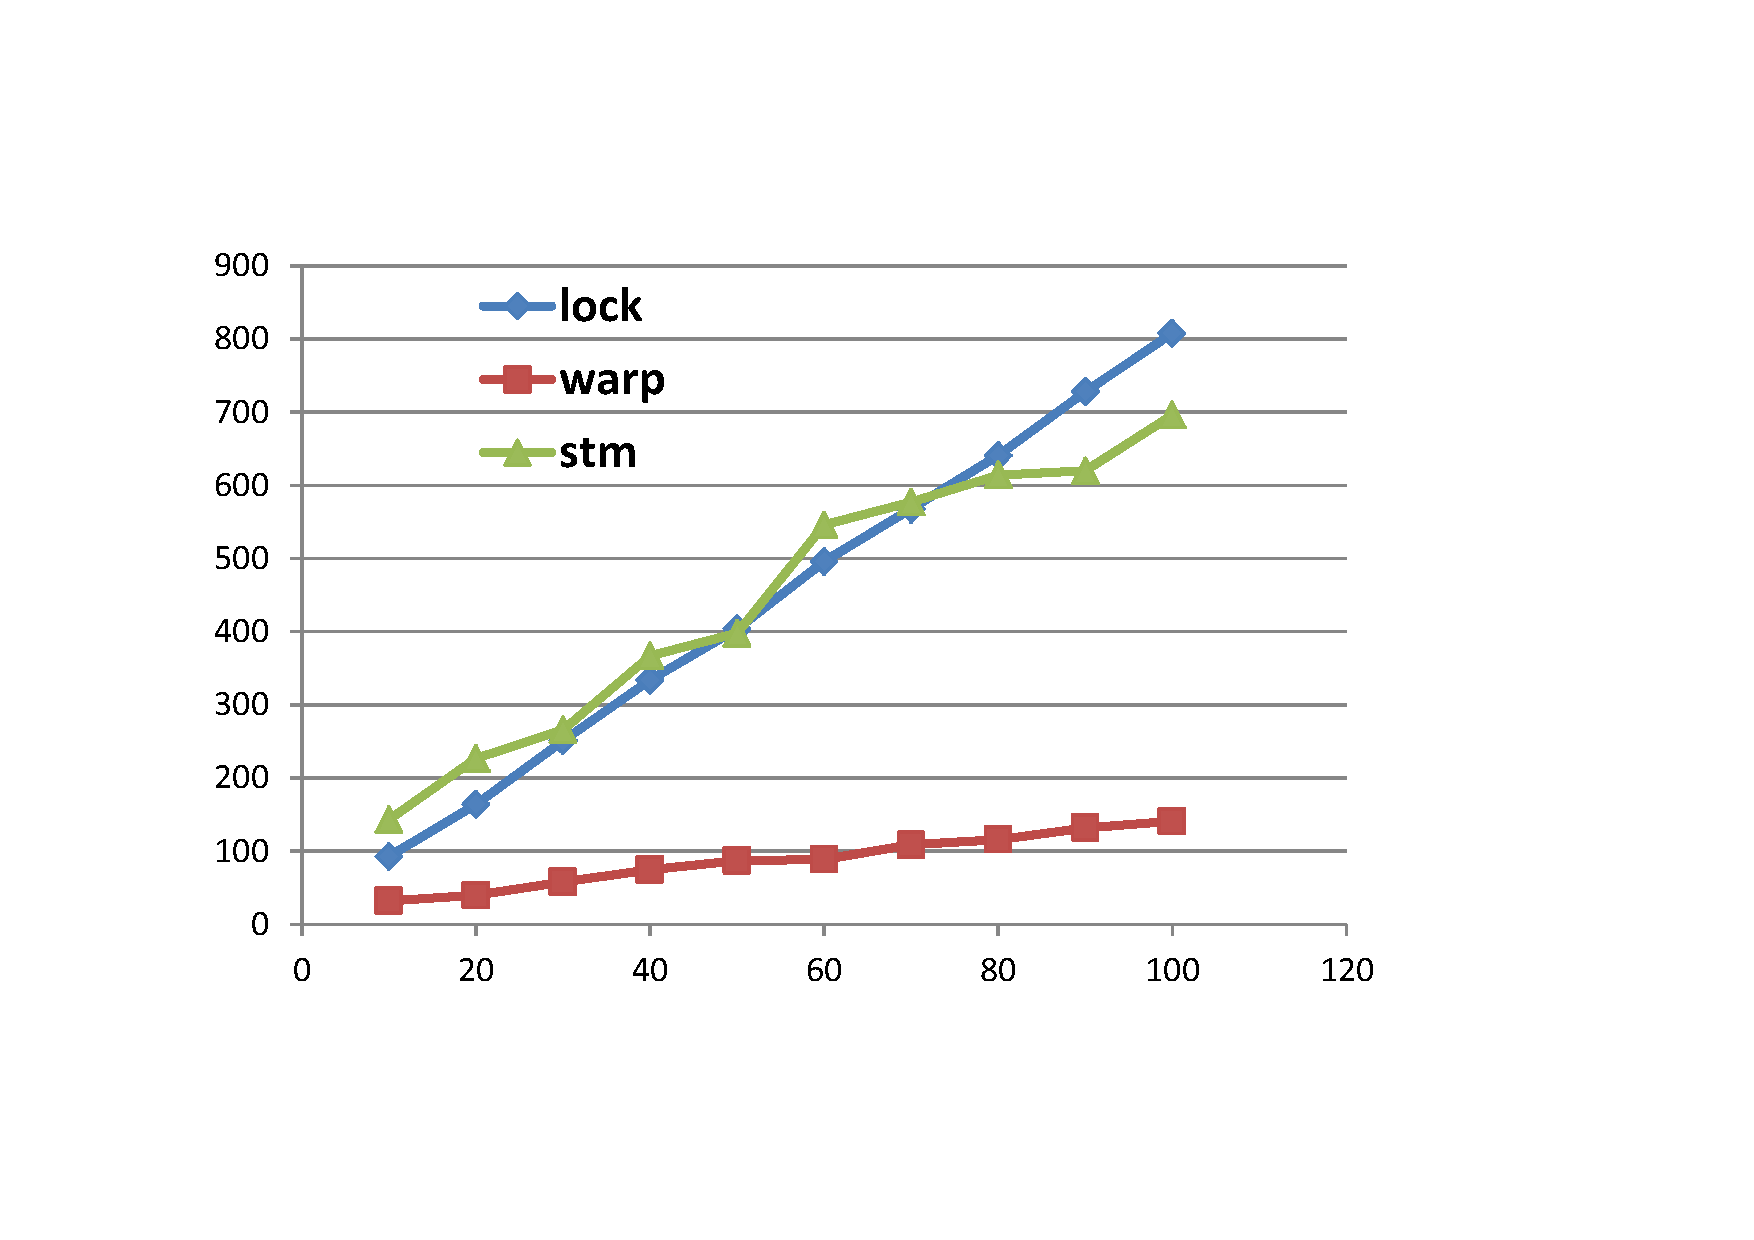
\includegraphics[width=0.33\textwidth]{../../eval/case2-varyIter.pdf}}
%\subfloat[{Case 2 with the increasing number of threads}]{\label{fig:case2Th}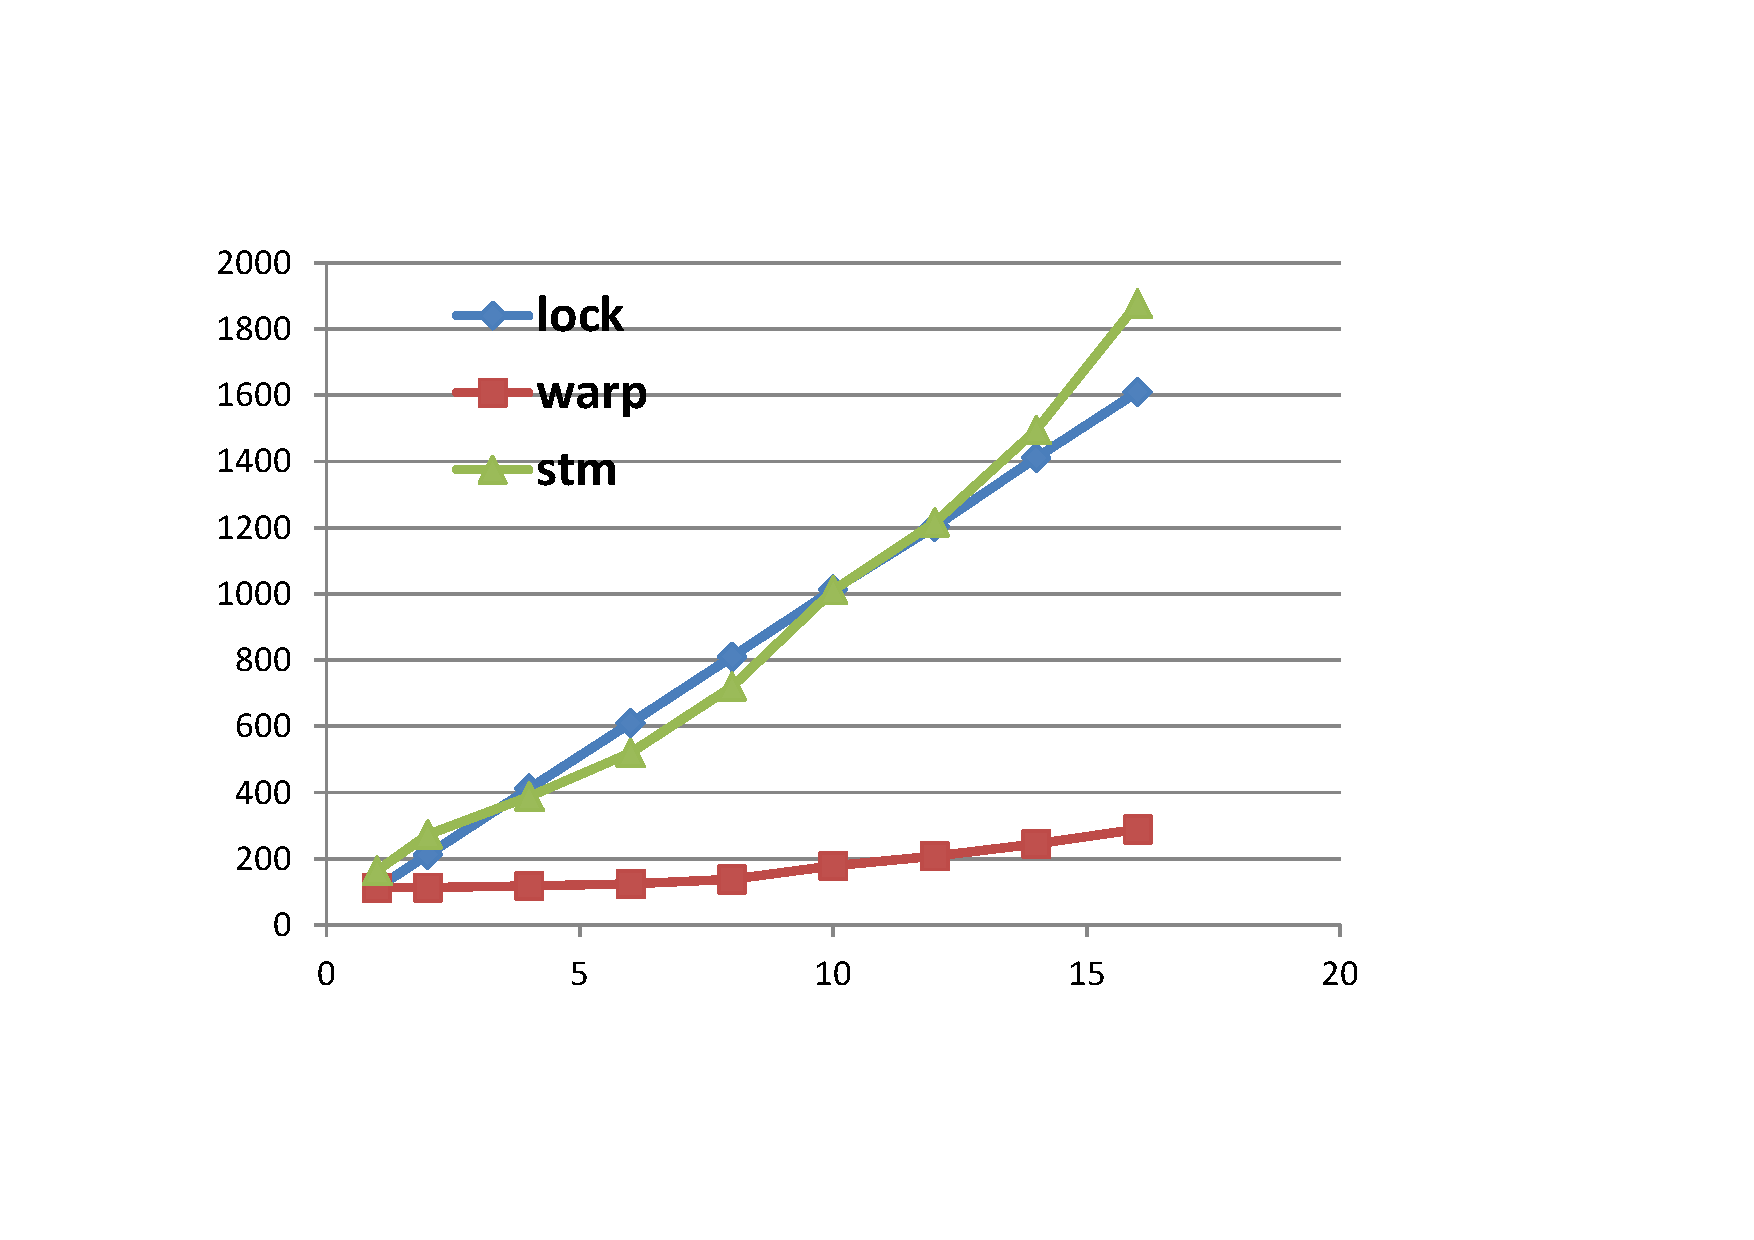
\includegraphics[width=0.33\textwidth]{../../eval/case2-varyThreads.pdf}}
%\\
%\subfloat[{Case 3 with the increasing workload}]{\label{fig:case3Iter}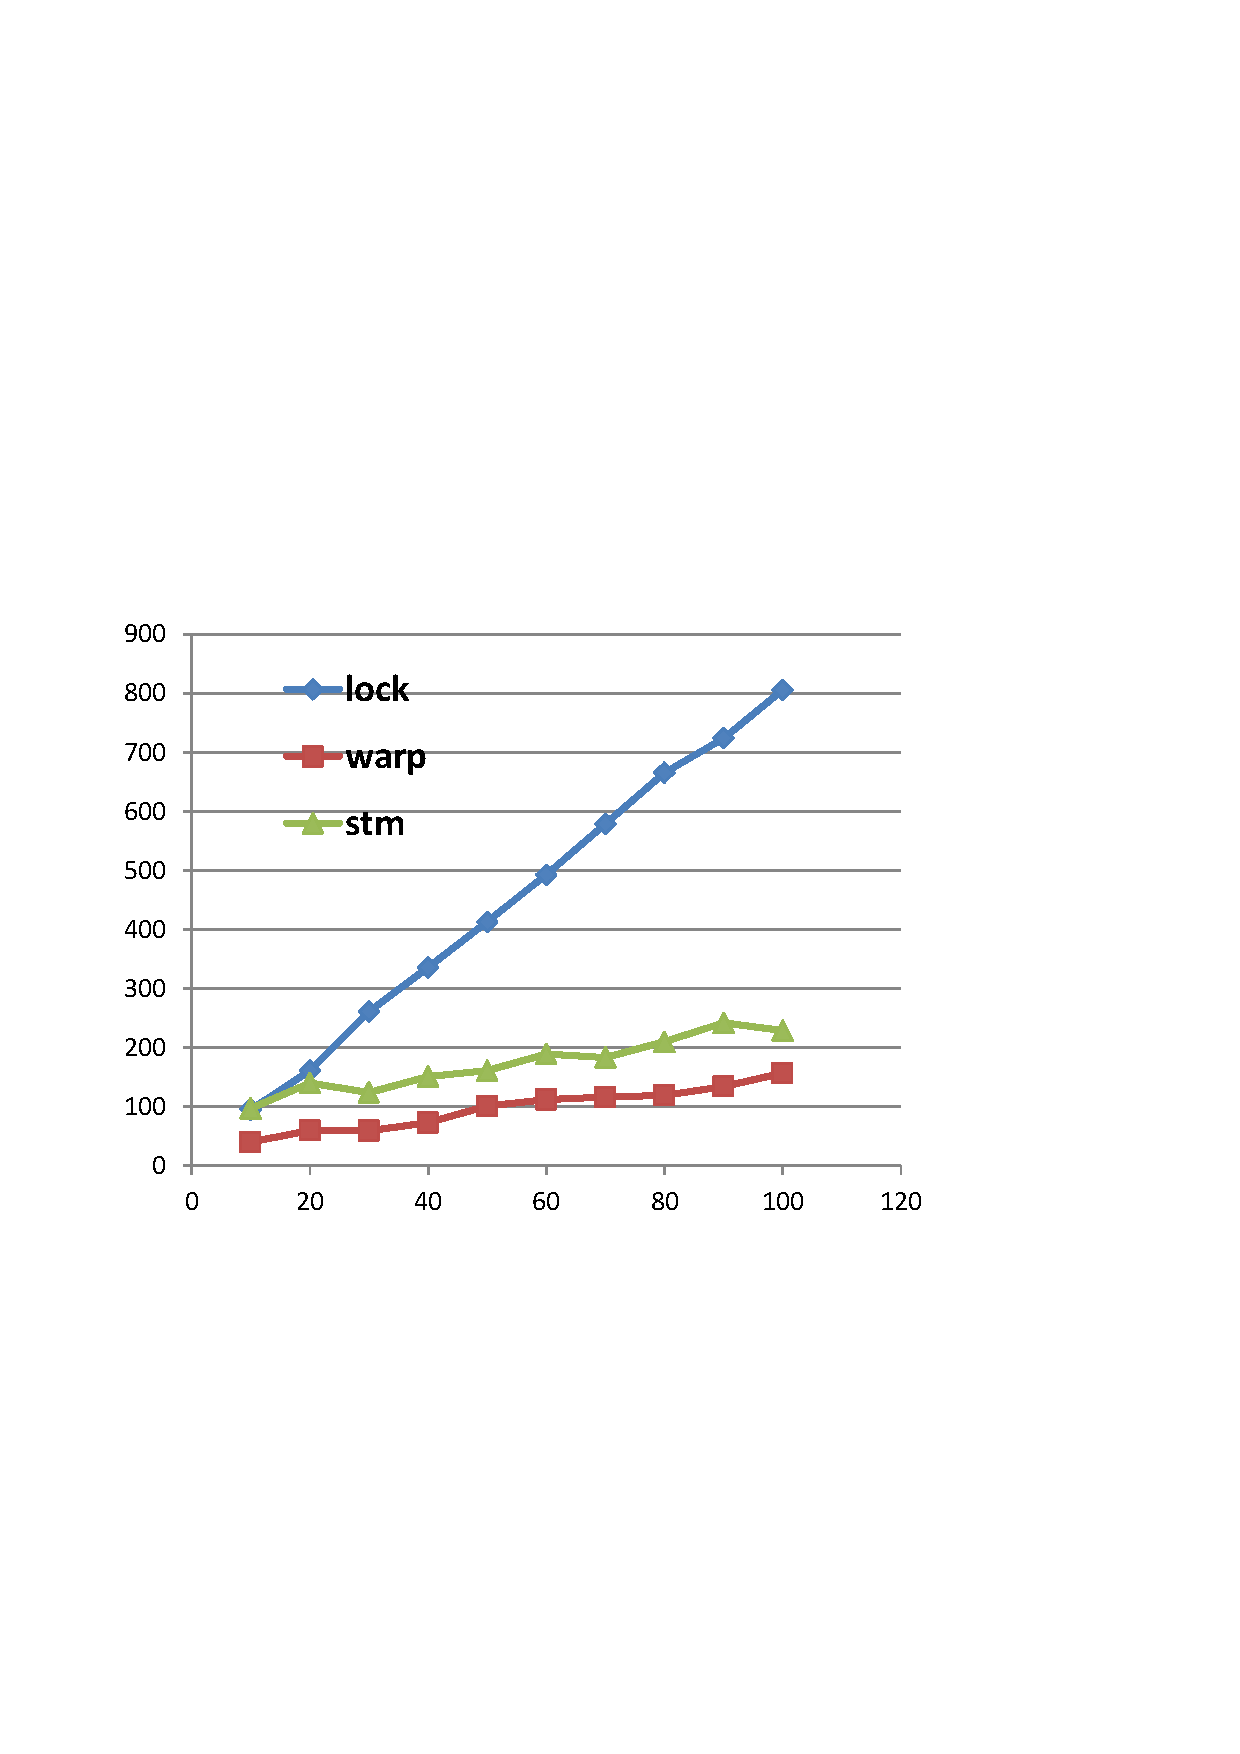
\includegraphics[width=0.33\textwidth]{../../eval/case3-varyIter.pdf}}
%\subfloat[{Case 3 with the increasing number of threads}]{\label{fig:case3Th}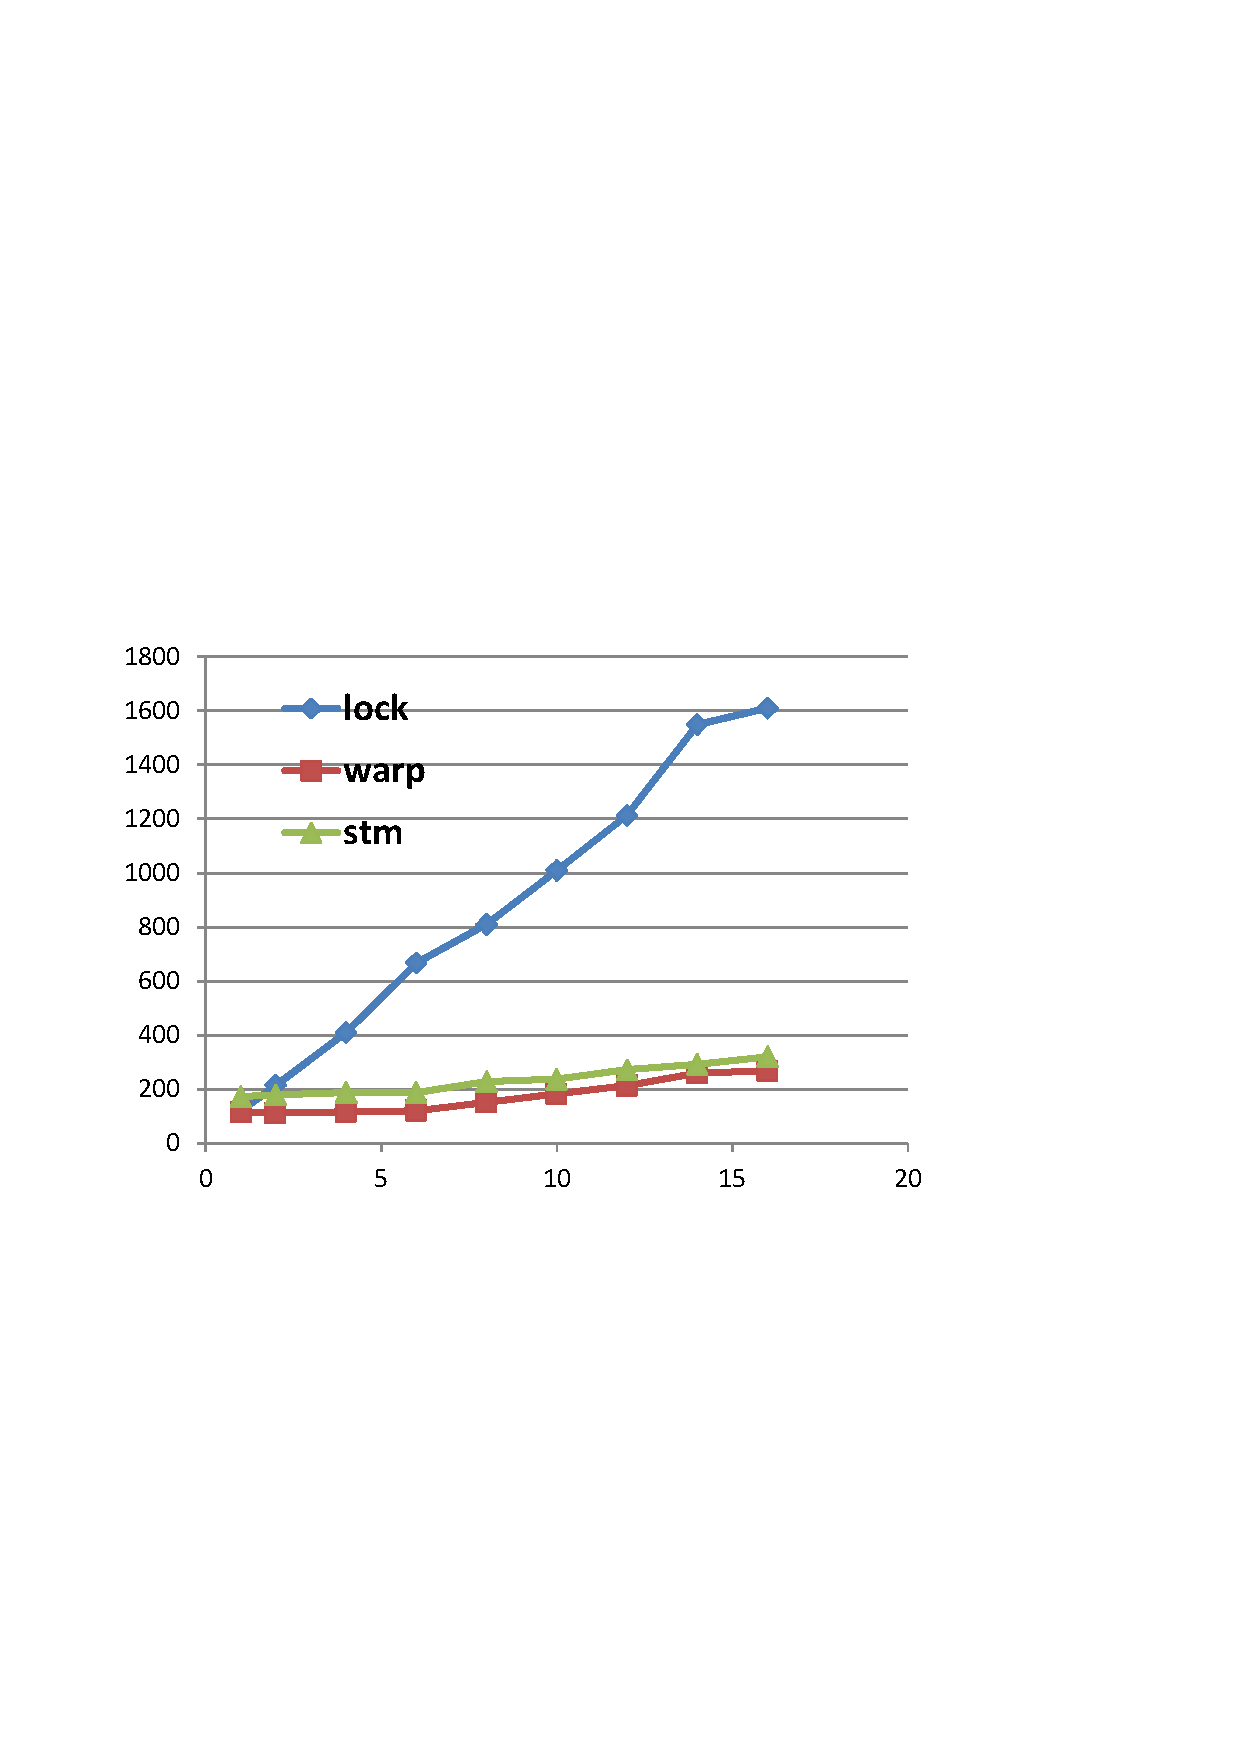
\includegraphics[width=0.33\textwidth]{../../eval/case3-varyThreads.pdf}}
%\\
%\subfloat[{Case 4 with the increasing workload}]{\label{fig:case4Iter}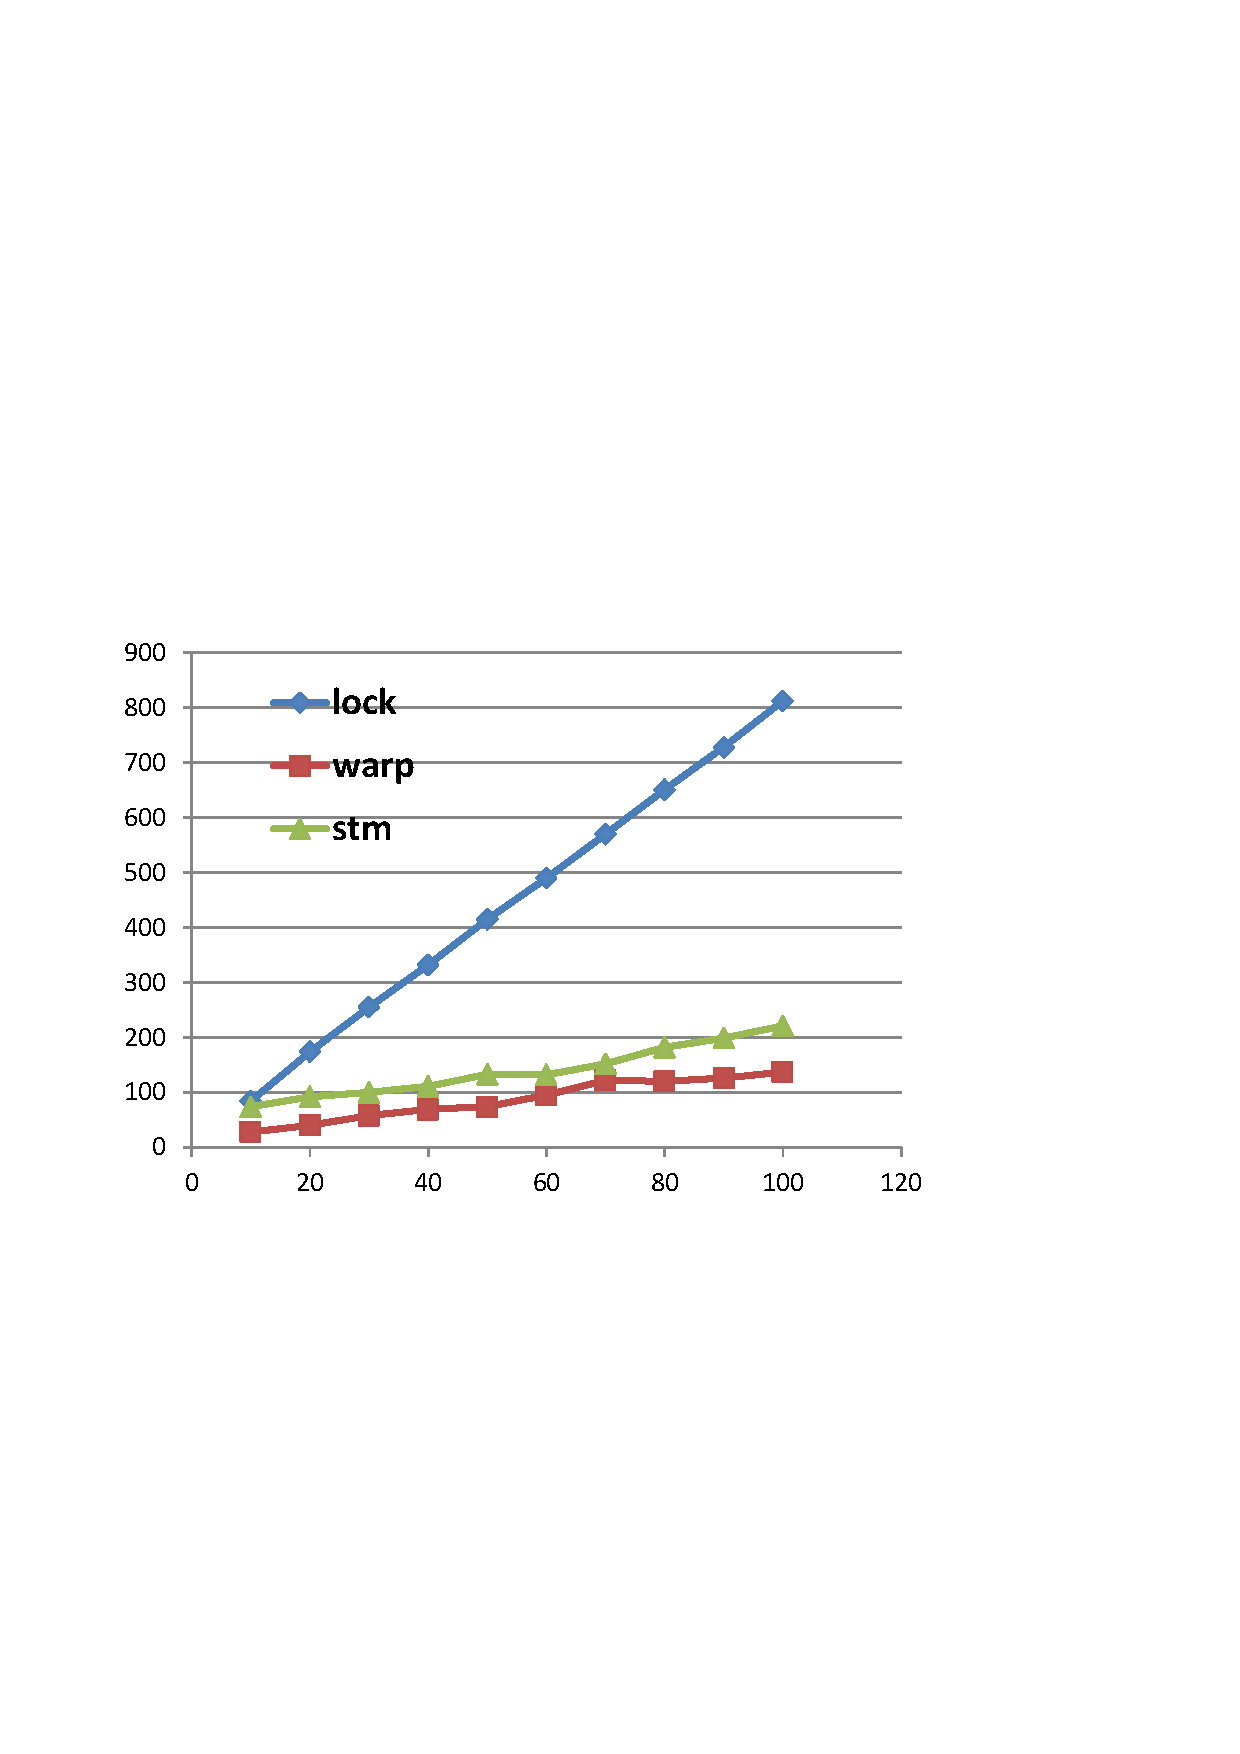
\includegraphics[width=0.33\textwidth]{../../eval/case4-varyIter.pdf}}
%\subfloat[{Case 4 with the increasing number of threads}]{\label{fig:case4Th}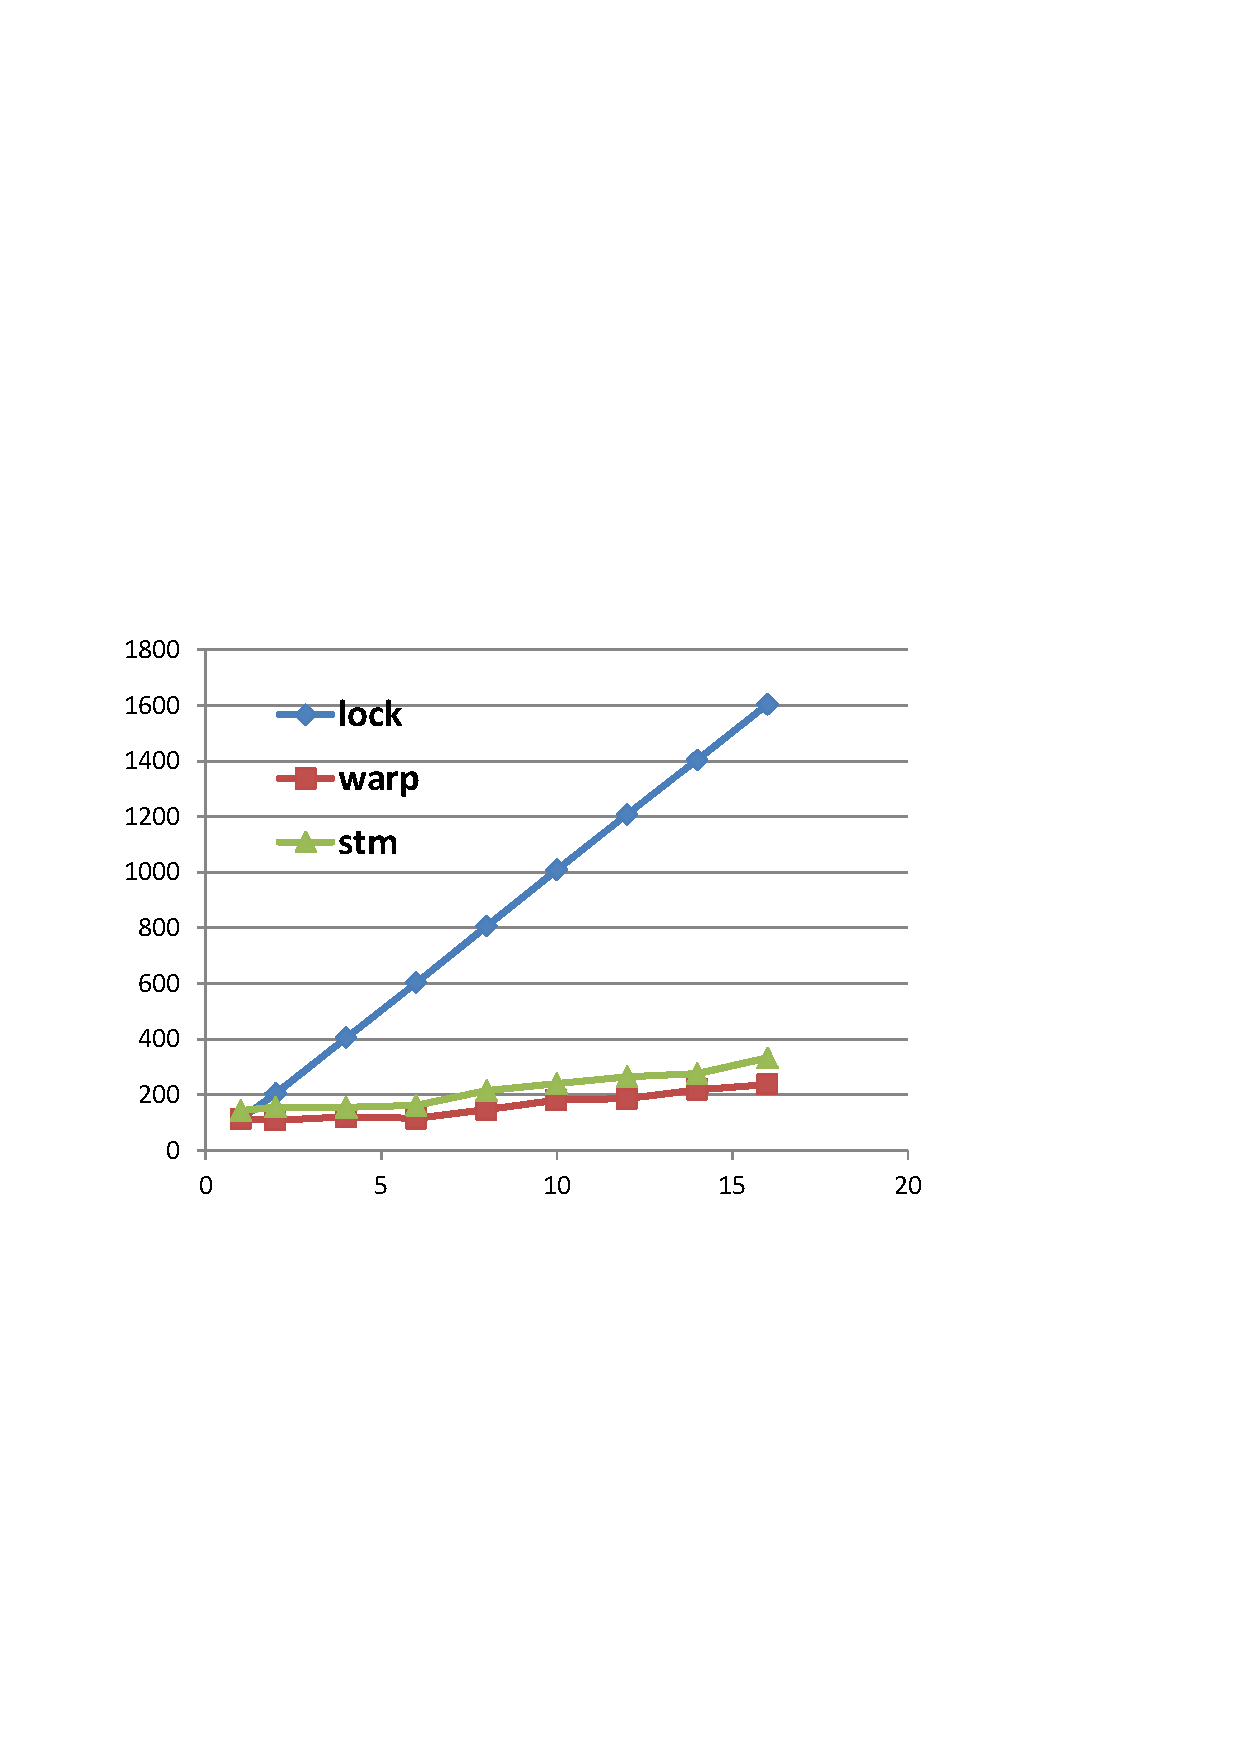
\includegraphics[width=0.33\textwidth]{../../eval/case4-varyThreads.pdf}}
%\\
%\subfloat[{Case 5 with the increasing workload}]{\label{fig:case5Iter}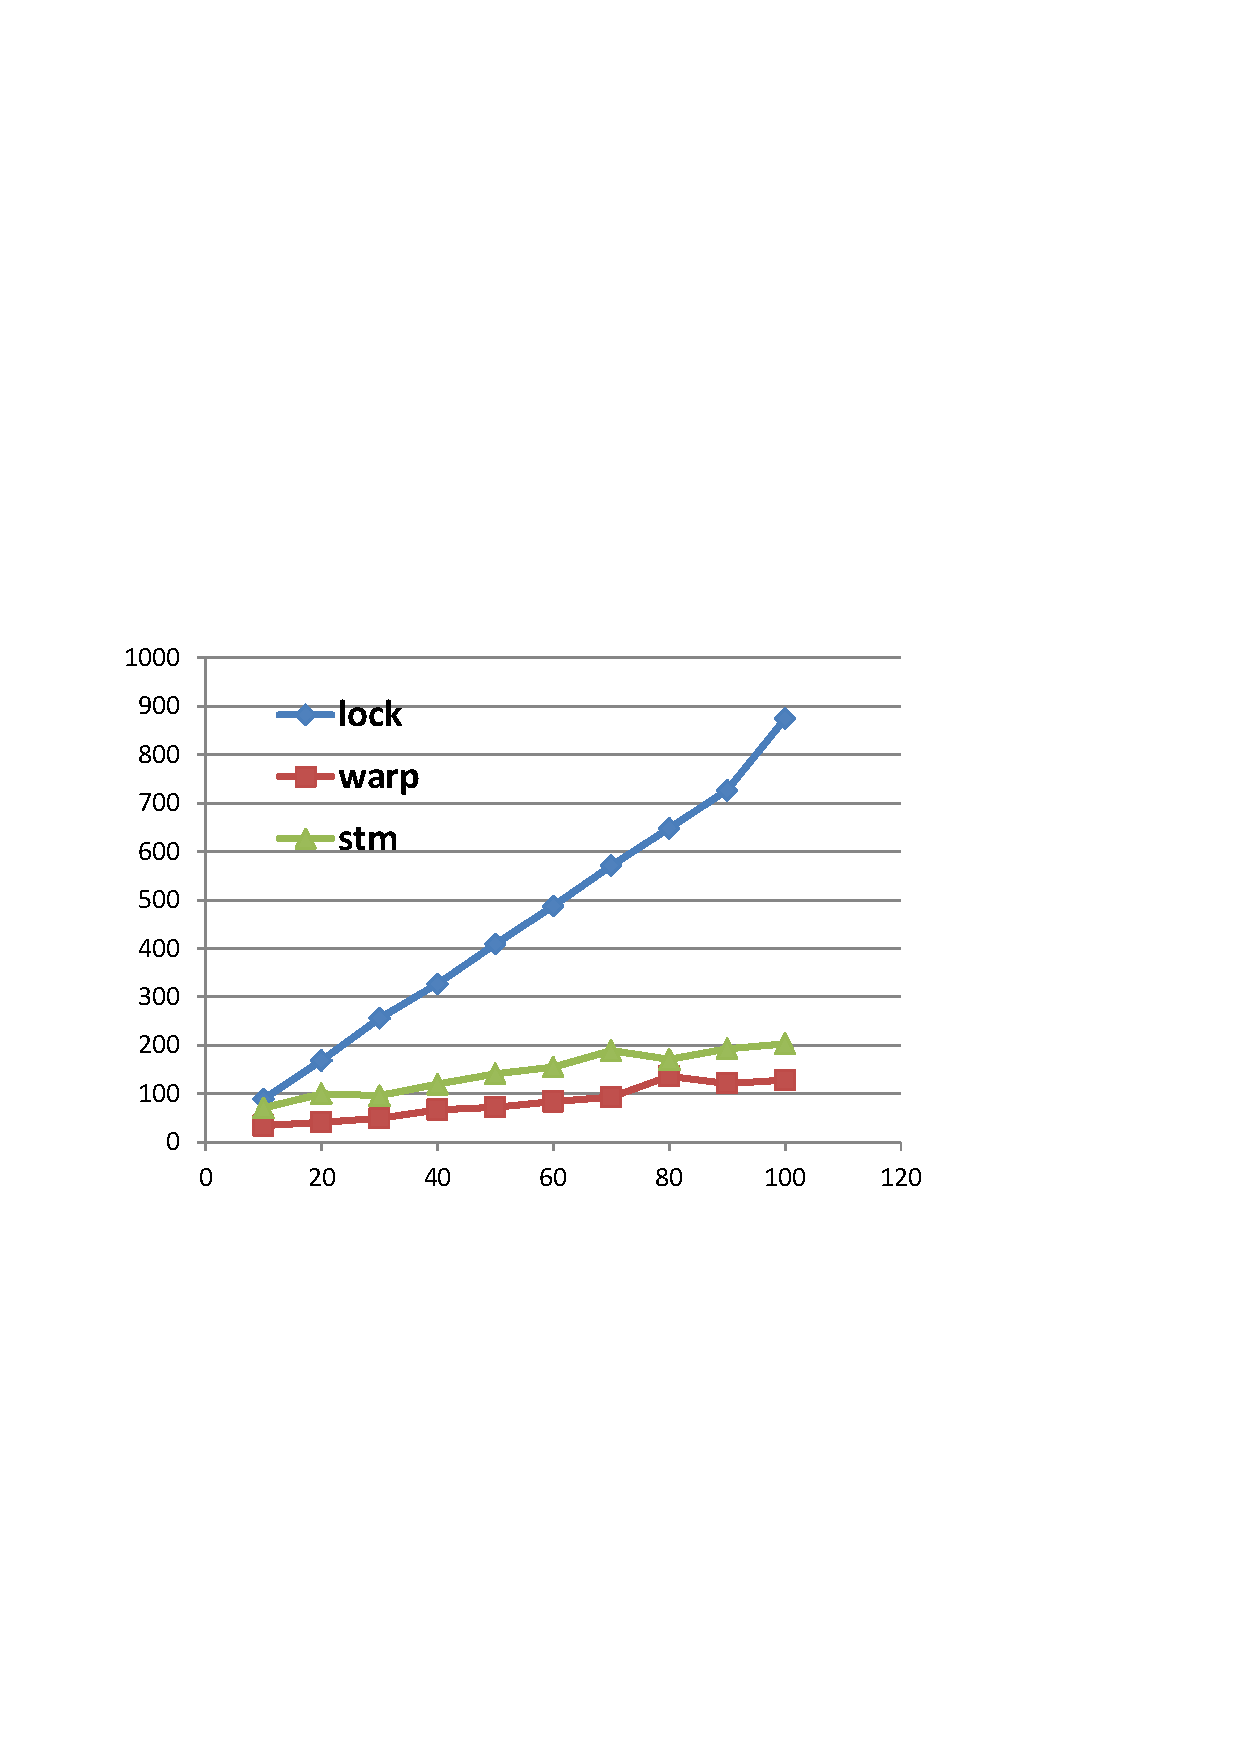
\includegraphics[width=0.33\textwidth]{../../eval/case5-varyIter.pdf}}
%\subfloat[{Case 5 with the increasing number of threads}]{\label{fig:case5Th}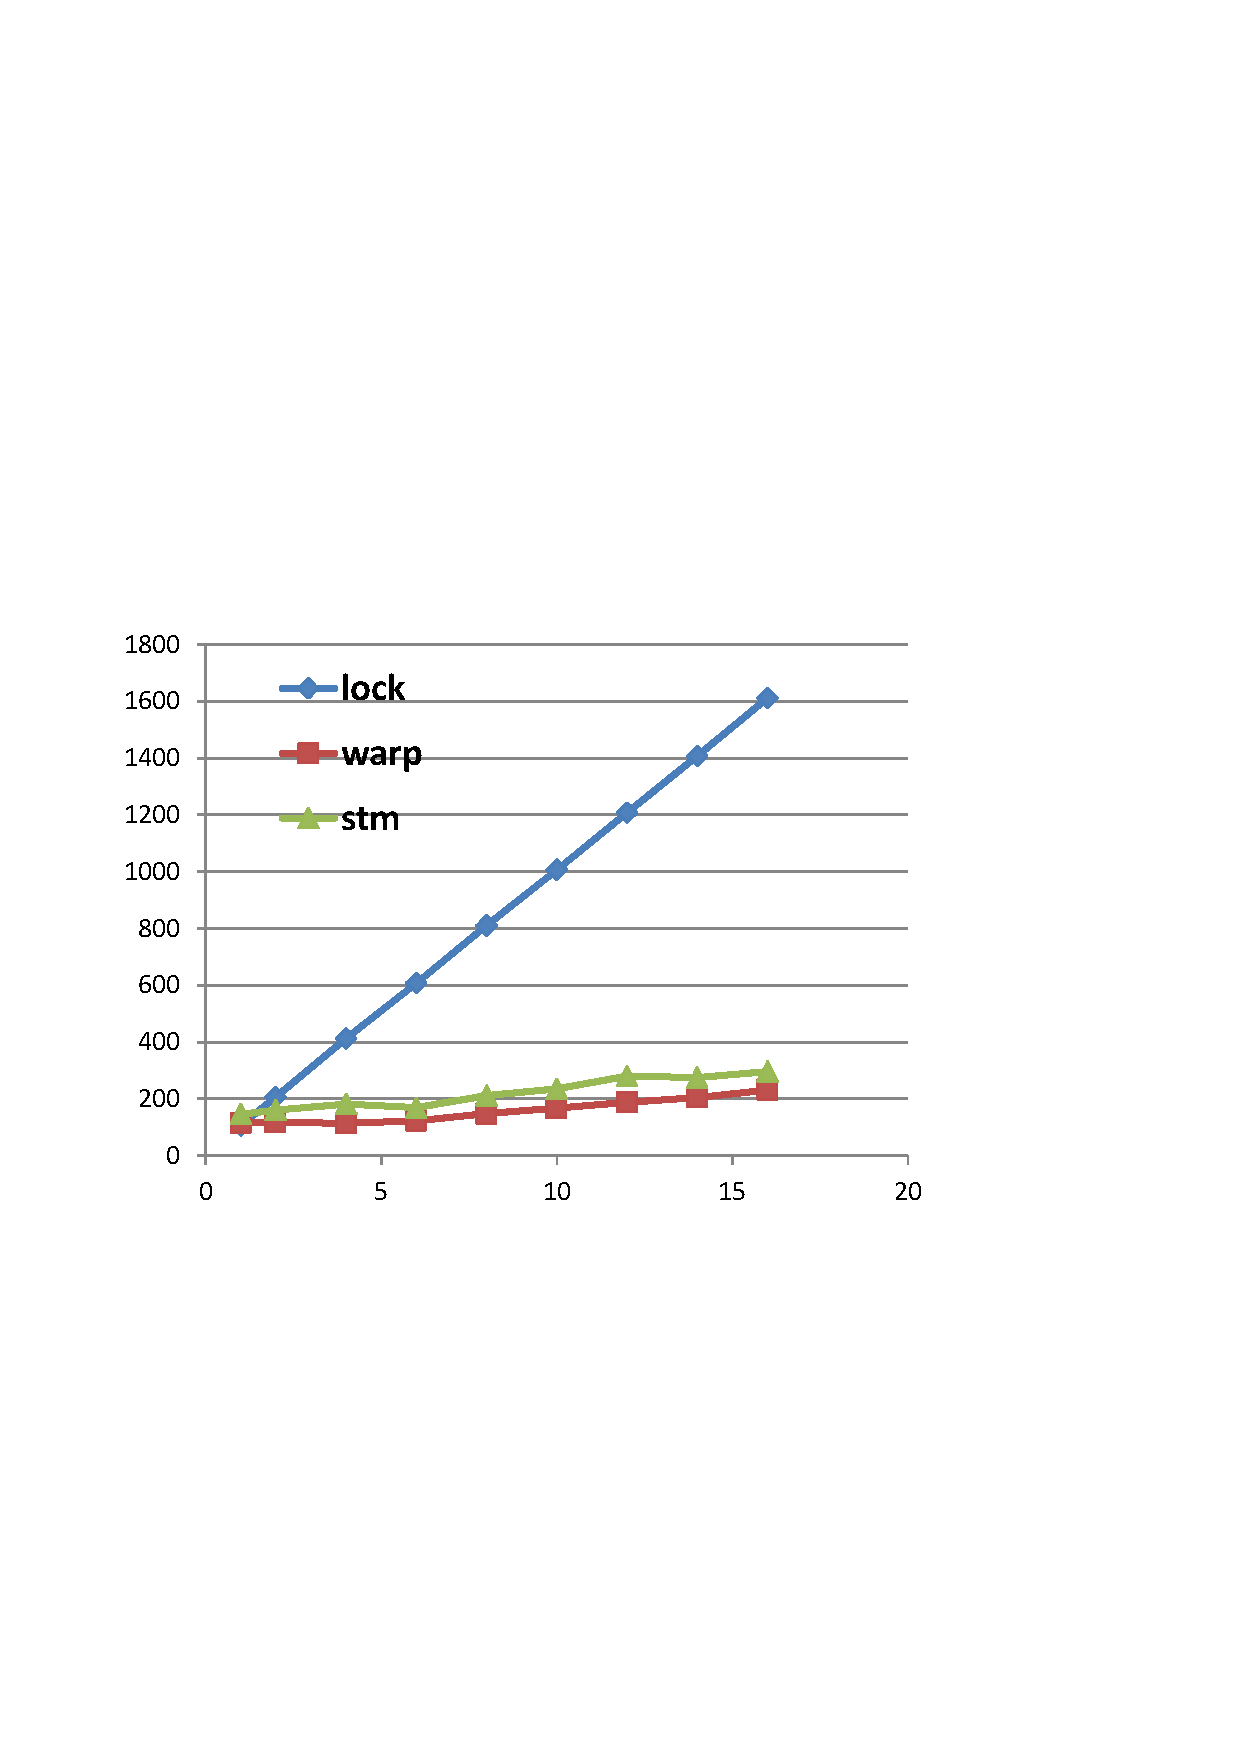
\includegraphics[width=0.33\textwidth]{../../eval/case5-varyThreads.pdf}}
%\caption{Performance Measurement}
%\label{fig:perf}
%\vspace{-1em}
%\end{figure*}









\section{Related work}
To our knowledge, existing solutions to the problem of correct synchronization assume either the ability to prevent bad interleavings or the ability to roll back execution. We focus our survey of related research on solutions for optimizing the rollback mechanism, and also discuss works on synchronization synthesis based on static program analysis.

\paragraph{Rollback optimizations.}
There are two main optimizations to decrease rollback overhead,
reducing either abort rate or the extent to which a conflicted
transaction rolls back. Different solutions have been proposed along
each of these directions~\cite{ppopp/HerlihyK08,Galois,TYFS:OOPSLA11}
and still others leverage available nondeterminism
\cite{TKS:OOPSLA13}. None of these approaches perform corrective
synchronization.
%
%Conflict detection is primarily based on violations of disjoint parallelism. That is, if two transactions perform simultaneous read/write or write/write accesses to the same memory location, then they are deemed conflicting. 
%
%An effective approach to mitigate false conflicts is to leverage the built-in guarantees of concurrent data structures \cite{ppopp/HerlihyK08,Galois,TYFS:OOPSLA11}. As an example, two {\sf ConcurrentHashMap} instances that perform {\sf put} operations involving different keys may still appear to conflict as they both access {\sf size}.
%
%Transactional boosting~\cite{ppopp/HerlihyK08} is a systematic methodology to specify the behavior of linearizable data-structure operations in terms of their semantic footprint. The Galois system \cite{Galois}, follows a similar approach with emphasis on the {\sf Graph} ADT. The Hawkeye tool~\cite{TYFS:OOPSLA11} detects impediments to parallelization accurately by mapping between the concrete and abstract representations of the data structure (albeit not its operations).
%
%In another study, Tripp et al.~\cite{TMFS:PLDI12} mine commutative behaviors involving \emph{multiple} operations out of execution traces of the program that appear to conflict when viewed at the granularity of individual operations. These are then translated into logical conditions used to avoid spurious conflicts in lazy STM.
%
%Another approach to reduce conflict is to leverage available nondeterminism \cite{TKS:OOPSLA13}. If a transaction can choose between nondeterministic behaviors (e.g., selecting among different paths between two graph nodes), then conflict is potentially reduced by directing the transaction toward a path where interference with other threads is less likely.
%
A well-known solution to restrict the extent to which a transaction rolls back is checkpointing \cite{spaa08a,Egwutuoha:2013}
%Checkpointing introduces the notion of a partial abort, where the transaction resumes from some intermediate point rather than fully resetting its execution and effects.
or nested transactions \cite{ont,beeri}.
%achieve a similar effect in that only the nested transaction, but not its parent transaction, aborts and restarts. Yet another mechanism to reduce rollback overhead is
Elastic transactions~\cite{FGG:DISC09} avoid wasted work by splitting into multiple pieces.  
%
The Push/Pull model \cite{KoskinenP15} also uses local/shared logs, and is flexible enough to express rollback-based transactions but nor corrective synchronization.
%. However, corrective synchronization is not expressible in Push/Pull. We introduce a new rule, {\sf corr}, and treat {\sf cmt} differently with the {\sf serpref} function.

\paragraph{Use of static analysis.} In our solution, static analysis is used to identify admissible shared-state configurations to correct to from a given input state. Multiple past works on synchronization synthesis have also relied on static analysis, albeit for the extraction of other types of information. We survey some of these works in the following.
%
Golan-Gueta et al.~\cite{GRSY:PLDI13} utilize static analysis to compute a conservative approximation of the possible actions that a transaction may perform in its future from a given intermediate point. This still pessimistic approach enables more granular synchronization compared to the worst-case assumption that the transaction may perform any action in its future.
%
Autolocker \cite{popl/McCloskeyZGB06} applies static analysis to determine a correct locking policy.
%, free of deadlocks and race conditions, given (i) a specification of pessimistic atomic sections and (ii) annotations that connect locks to shared sections. The analysis, encoded as a type system, guarantees deadlock and race freedom.
%
Hawkins et al. \cite{HawkinsAFRS12}
%propose a system that transforms a program consisting, in part, of concurrent relations into a program where the relations are represented as concrete concurrent data structures, as well as locks, that together
ensure correct synchronization by construction.
%They guarantee serializability and deadlock freedom.
%
Prountzos et al. \cite{PrountzosMPM11} optimize the Galois system \cite{Galois} via static shape analysis \cite{MoolyToplas}.
%They apply the TVLA system to identify fail-safe points during the transaction's execution, beyond which neither backup nor conflict detection are necessary. 

%This gives rise to two optimizations: (i) the transaction does not need to back up modified data, and (ii) redundant conflict checking can be eliminated. In Proznos et al.'s solution, the shape analysis, which is parametric in essence, is instantiated via a predicate discovery algorithm that exploits common patterns of data-structure usage.




%%% Local Variables:
%%% mode: latex
%%% TeX-master: "paper"
%%% End:


\section{Conclusion and Future Work}

We have presented an alternative to the lock- and retry-based synchronization methods, which we dub \emph{warping}. The key insight is to correct a bad execution, rather than retrying the involved transaction(s), which is expensive, or preventing bad behaviors from arising in the first place, which often obviates the performance advantages of concurrent execution.

In our implementation of the warping approach, we utilize static analysis to compute candidate fixes. Then, at runtime, we track lightweight information to verify serializability, and compute an appropriate fix if needed. Our evaluation over methods from five popular concurrent libraries demonstrates the viability of warping as an alternative, or complement, to existing synchronization approaches. 

In the future, we intend to develop compositional synchronization methods that integrate warping with lock- and STM-based synchronization. We also plan to explore other ways of achieving completeness. 

{%\footnotesize\linespread{0.9}
\bibliographystyle{acm}
%\bibliography{nopages}
\bibliography{biblio}
}


\newpage
\appendix
\section{Case Studies}
\label{appendix:casestudies}

\subsection{Apache Tomcat}

\subsubsection{Transaction 1}
\begin{lstlisting}
Attribute removeAttribute(String name){
	Attribute val = null;
	found = attr.containsKey(name) ;
	if (found) {
		val = attr.get(name);
		attr.remove(name);
		}
	return val;
}
\end{lstlisting}

%
%**********************
%
%Our code
%
%**********************
%
%\begin{lstlisting}
%ret=null;
%if(map.containsKey(key)) {
%	ret=map.get(key);
%	map.remove(key);
%}
%return ret;
%\end{lstlisting}

\subsubsection{Transaction 2}
\begin{lstlisting}
boolean removeAttribute(String name, Attribute value){
	boolean replaced = false;
	oldValue = attributes.get(name);
	if (oldValue != null)
		replaced = true;
	attributes.put(name, value);
	return replaced;
}
\end{lstlisting}


%**********************
%
%Our code
%
%**********************
%
%\begin{lstlisting}
%ret=map.containsKey(key);
%map.put(key, value);
%return ret;
%\end{lstlisting}

\subsection{dyuproject}

\subsubsection{Transaction 1}
\begin{lstlisting}
public Convertor getConvertor(Class<?> clazz, boolean create, boolean addClass) {
	Convertor convertor = (Convertor)_convertors.get(clazz.getName());
	if(convertor==null && create) {
		convertor = newConvertor(clazz, addClass);
		_convertors.putIfAbsent(clazz.getName(), convertor);
	}
	return convertor;
}
\end{lstlisting}


%**********************
%
%Our code
%
%**********************
%
%\begin{lstlisting}
%value=map.get(key);
%if(value==null && b) {
%	value=new Value();
%	map.putIfAbsent(key, value);
%}
%retrun value;
%\end{lstlisting}

\subsubsection{Transaction 2}
\begin{lstlisting}
protected Convertor getConvertor(String className) {
	Convertor convertor = (Convertor)_convertors.get(className);
	if(convertor==null) {
		Class<?> clazz = StandardJSON.loadClass(className);;
		convertor = clazz==null ? UNRESOLVED_CONVERTOR : newConvertor(clazz);
		_convertors.putIfAbsent(className, convertor);
	}
	return convertor;
}
\end{lstlisting}


%**********************
%
%Our code
%
%**********************
%
%\begin{lstlisting}
%value=map.get(key);
%if(value==null) {
%	value=new Value();
%	map.putIfAbsent(key, value);
%}
%return value;
%\end{lstlisting}

\subsection{Flexive}

\subsubsection{Transaction 1}
\begin{lstlisting}
public static FxValueRenderer getInstance(FxLanguage language) {
	if (language == null) {
	// default renderer always exists
	return renderers.get(DEFAULT);
	}
	if (!renderers.containsKey(language)) {
		renderers.putIfAbsent(language, new FxValueRendererImpl(language));
	}
	return renderers.get(language);
}
\end{lstlisting}

%
%**********************
%
%Our code
%
%**********************
%
%\begin{lstlisting}
%if(!map.containsKey(key)) {
%	loc_w=new Value();
%	map.putIfAbsent(key, loc_w);
%}
%return map.get(key)"
%\end{lstlisting}

\subsubsection{Transaction 2}
\begin{lstlisting}
void addRenderer(FxLanguage language, Class<T> valueType, FxValueFormatter<DT, T> formatter) {
	renderers.putIfAbsent(language, new FxValueRendererImpl(language));
	renderers.get(language).put(valueType, formatter);
}
\end{lstlisting}

%
%**********************
%
%Our code
%
%**********************
%
%\begin{lstlisting}
%loc_w=new Value();
%map.putIfAbsent(key, loc_w);
%loc_w=map.get(key);
%\end{lstlisting}

\subsection{Gridkit}
\subsubsection{Transaction 1}
\begin{lstlisting}
protected Object internalDeserialize(PofReader in) throws IOException {
	Class<?> type = in.getPofContext().getClass(in.getUserTypeId());
	ObjectFormat format = formats.get(type);
	if (format == null) {
		try {
			format = new ObjectFormat(type);
		} catch (Exception e) {
			throw new IOException("Failed to create reflection format for " + type.getName(), e);
		}
	formats.put(type, format);
	}
	Object result = resolve(format.deserialize(in));
	return result;
}
\end{lstlisting}

%
%**********************
%
%Our code
%
%**********************
%
%\begin{lstlisting}
%if(map.containsKey(key)) {
%	value=new Value();
%	map.put(key, value);
%	ret=null;
%} else
%	ret=map.get(key);
%return ret;
%\end{lstlisting}

\subsubsection{Transaction 2}
\begin{lstlisting}
protected void internalSerialize(PofWriter out, Object origValue) throws IOException {
	Object value = replace(origValue);
	Class<?> type = value.getClass();
	ObjectFormat format = formats.get(type);
	if (format == null) {
		try {
			format = new ObjectFormat(type);
		} catch (Exception e) {
			throw new IOException("Failed to create reflection format for " + type.getName(), e);
			}
		formats.put(type, format);
	}
	format.serialize(out, value);
}
\end{lstlisting}


%**********************
%
%Our code
%
%**********************
%
%\begin{lstlisting}
%if(map.containsKey(key))
%	value=new Value();
%map.put(key, value);
%\end{lstlisting}

%\section{Complete \PMPY{} rules}
%\begin{figure*}
\figboxB{\footnotesize
\Tboxed{(a) \PMPY{} {\bf Machine Rules} $\pmpyreduce$}
$$
\infer[\text{\FIN{}}]{
  \Ts_1\cdot\csl\cdot\Ts_2,G \pmpyreduce
  \Ts_1\cdot \Ts_2,G
}{\nothing{c}}
\hspace{0.1in}
\infer[\text{\FORK{}}]{
  \Ts_1\cdot\cslC{c}\cdot\Ts_2,G \pmpyreduce
  \Ts_1\cdot\cslC{c_1}\cdot\cslC{c_2}\cdot\Ts_2,G
}{\tstep{c}{\fork{c_1}}{c_2}}
$$
$$
\infer[\text{\LOCAL{}}]{
  \Ts_1\cdot\cslCS{c_1}{\sigma_1}\cdot\Ts_2,G \pmpyreduce
  \Ts_1\cdot\cslCS{c_2}{\sigma_2}\cdot\Ts_2,G 
}{\tstep{c_1}{\localR}{c_2} & R\ \sigma_1\ \sigma_2}
$$
$$
\infer[\text{\BEGIN{}}]{
  \Ts_1\cdot\cslC{c_1}\cdot\Ts_2,G \pmpyreduce
  \Ts_1\cdot\cslC{(\tx{c},c_2)}\cdot\Ts_2,G
}{\tstep{c_1}{\tx{c}}{c_2}}
\hspace{0.1in}
\infer[\text{\CMT{}}]{
   \Ts_1\cdot\cslC{(\tx{c},c_1)}\cdot\Ts_2,G \pmpyreduce
   \Ts_1\cdot\cslC{c_1}\cdot\Ts_2,G'
}{
  \nothing{c}  & L \subseteq G & \committ(G,L,G')
}
$$
\begin{center}
\begin{tabular}{rl}
\begin{minipage}{3.5in}
$$
\infer[\text{\STEP{}}]{
   \Ts_1\cdot\cslC{(\tx{c},c_1)}\cdot\Ts_2,G \pmpyreduce
   \Ts_1\cdot\cslCSL{(\tx{c'},c_1)}{\sigma'}{L'}\cdot\Ts_2,G'
}{
  \CSL, G
  \Dir
  \CpSpLp, G'
}
$$
\end{minipage}
&
\begin{minipage}{3.1in}
%The {\sc PPTxEnd} rule involves predicate \textsf{cmt}, defined as follows:
where $\textsf{cmt}(G_1,L_1,G_2) \equiv$\\
$\;G_2 \;=\; \textsf{map } \left(\lambda\ (\op,g).\ 
     \begin{cases}
       (\op,\gCommitted) & \text{if } \op \in \pushed{L_1} \\
       (\op,g) & \text{ otherwise}
       \end{cases}
       \right) G_1
$
\end{minipage}
\end{tabular}
\end{center}
\medskip
\noindent
\Tboxed{(b) \PMPY{} {\bf Step Rules} $\Dir$}
\ottusedrule{\ottdruleapp{}}
\ottusedrule{\ottdruleunapp{}}
\bigskip
\ottusedrule{\ottdrulepush{}}
\ottusedrule{\ottdruleunpush{}}
\bigskip
\ottusedrule{\ottdrulepull{}}
\ottusedrule{\ottdruleunpull{}}
}
\caption{\label{fig:ott}
(a) The machine reductions of \PMPY{}. 
(b) The \PMPY{} rules.
  Notations $\setminus,\notin,\cdot,\subseteq$ are all lifted to
  lists where equality is given by $\opid$s. 
We will refer to the premise criteria of each rule as, for example, ``\critPUSHii.'' 
Criteria that are written in \gray{gray font} are not strictly
necessary. See inline discussion.}
\end{figure*}


%\section{First Sketch}

\begin{figure}
%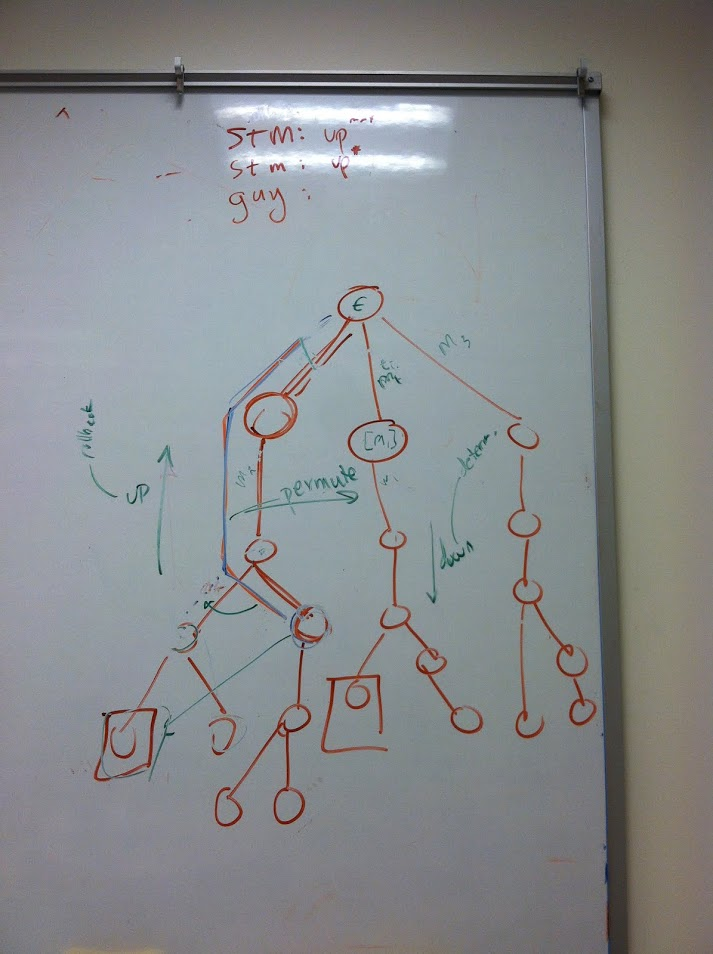
\includegraphics[width=\columnwidth]{tree.jpg}
tree.jpg
\caption{An example}
\label{fig:example}
\end{figure}

We start with a description of all possible interleaved executions of some bounded number of threads, as shown in Figure \ref{fig:example}. Some of the leaf nodes denote admissible final states for the interleaved execution. The rest are inadmissible final states.

A generic concurrent system may produce both admissible and inadmissible executions. Two main approaches have been adopted to produce only admissible executions:
\begin{itemize}
\item apply synchronization to restrict the available parallelism and drive the system only into the admissible executions, and
\item rollback the execution when the system falls into an inadmissible executions, and re-execute the program (sometimes driving the system to avoid to fall back to the inadmissible case already explored).
\end{itemize}

We would like to optimize two properties:
\begin{itemize}
\item Utilization of available parallelism, which is counted as the number of admissible paths that synchronization permits
\item Overhead, which is counted as the number of operation/state reversals that synchronization may force to (re)direct execution toward an admissible final state
\end{itemize}

\todo{for now i guess we just let an operation have unit cost. can
  worry about cost models later}



Our idea is to create a calculus founded on three operations:
\begin{itemize}
\item[Execute] forward execution step
\item[Rollback] local rollback
\item[Permute] a jump to another branch that reflects the same history of operations (but differs in terms of the order of execution of the operations)
\end{itemize}

Once we recognized we fall into an inadmissible execution, our goal is to perform some operations in order to fall into an admissible execution preserving the observable behaviors.
This leads us to two main concepts:
\begin{itemize}
\item What executions are admissible? (in the rest of the paper, we will adopt the classical idea of Software Transaction Memory)
\item What behaviors of an execution are observable? (in the rest of the paper, we will consider final states as the observable behaviors of an execution)
\end{itemize}

We can plug in our approach different definitions of admissible executions, and observable behaviors.

In addition, we want to formalize Permute reaching a node in the tree that is at the same level of the current one. In this way, we do not rollback the execution, but indeed we advance it by one step as we would do if we were in an admissible execution. Intuitively, this means that our permute can be simulated by $n$ rollbacks followed by $m$ execution steps, with $m==n$\footnote{We discussed also the case in which $m>n$, but we are not yet sure if this case will be never interesting}.

\begin{figure}
\begin{lstlisting}
T1:
	put(k,v)
	get(k)

T2:
	remove(k)
\end{lstlisting}
\caption{The running example}
\label{lst:runningexample}
\end{figure}

\begin{figure}[ht]
%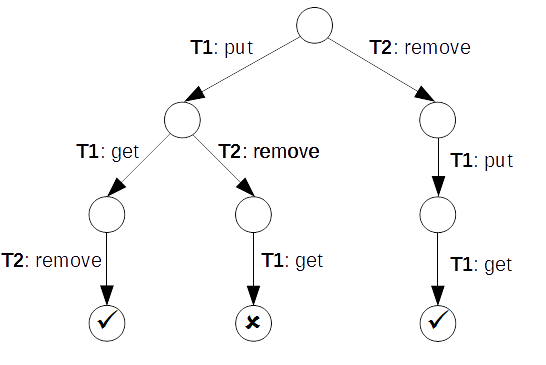
\includegraphics[width=\columnwidth]{treerunningexample.png}
treerunningexample.png
\caption{The tree of executions of the running example}
\label{fig:treerunningexample}
\end{figure}

Consider for instance the running example in Figure \ref{lst:runningexample}.
Figure \ref{fig:treerunningexample} depicts the tree of all possible executions of the running example. We consider the first and last execution as admissible, while the second one is not. This is a quite standard assumption for our running example: The two instructions of T1 conflict with the instruction of T2 (they all work on the same collection and on the same key). Therefore, the system should not allow T2 to execute its instruction if T1 has execute the first instruction but not the second one yet. This is usually achieved in two ways:
\begin{itemize}
\item by synchronization mechanisms (e.g., locks) providing mutual exclusion between T1 and T2, or
\item by rolling back the execution if the system falls into the second path and when executing remove.
\end{itemize}

Instead, we propose a novel approach.
Consider the second path, and the situation in which we have already exposed history \statement{[T1: put, T2: remove]}.
If we refrain from executing remove (that is, we replace it with a skip statement), we would apply a Permute step, that would yield us to the history	\statement{[T2: remove, T1: put]}

In this way, the entire execution becomes \statement{[T2: remove, T1: put, T1: get]} that is an admissible execution.

Note that in contrast with Rollback and Execute, Permute requires an algebraic specification that permits efficient (bounded) editing of the state reflected by \statement{[T1: put, T2: remove]} to arrive at \statement{[T2: remove, T1: put]}.




\section{Permuting the execution -- previous}
The goal of our work is to try to \emph{redirect} a bad execution into a good one by simulating the good trace up to that point. At a given point of an execution, we suppose that we can observe only two things:
\begin{enumerate}
\item where the execution of each transaction is. This can be formalized as $\getTransactionPoints{\tau} = [\statement{t} \mapsto \max(\indexes{\statement{t}}{\tau}) : \statement{t} \in \cset{T}]$
where $\cset{T}$ contains all the identifiers of the transactions in the execution $\tau$, and $\indexes{\statement{t}}{\tau}=\{\cel{i} : \exists \cel{\sigma}_j \to_{(\statement{t}, \cel{i})} \cel{\sigma}_{j+1} \in \tau\}$
\item what we can observe on the last state of the trace. The observational portion of the state is given by a function $\observe{\sigma}$.
\end{enumerate}

Given a bad trace $\sigma_0 \to \cdots \to \sigma_i$ we want to find a good trace $\sigma'_0 \to \cdots \to \sigma'_j$ such that
\begin{enumerate}
\item $\getTransactionPoints{\sigma_0 \to \cdots \to \sigma_i} = \getTransactionPoints{\sigma'_0 \to \cdots \to \sigma'_j}$
\item $\observe{\sigma_0}=\observe{\sigma'_0}$
\item $\observe{\sigma'_j} = \observe{f(\sigma_i)}$ where $f$ is a function that \emph{adjusts} the state of the bad execution to fall into the good execution.
\end{enumerate} 

The two parameters of our framework are $f$ (and a key component is how to compute it) and $\observe{\sigma}$. We suppose that $\observe{\sigma}$ returns the portion of the state that influences what is observable "through" the semantics. This means that if we take two states equivalent modulo observability and we perform the semantics of a statement, we obtain two states that are equivalent modulo observability. Formally,
\[
\begin{array}{c}
\forall \sigma, \sigma' \in \cstates : \observe{\sigma}=\observe{\sigma'} , \forall \statement{s} \in \statements : \langle \statement{s}, \sigma \rangle \to \sigma_1, \langle \statement{s}, \sigma' \rangle \to \sigma'_1\\
\Downarrow\\
\observe{\sigma_1}=\observe{\sigma'_1}\\
\end{array}
\]

Based on the permutation function $f$ we define the semantics $\csemantics{S_{P}}{\statement{p}, \sigma_0}$ that, if the execution falls into a bad trace, redirects the execution into a good trace by applying $f$.\todo{Formalize it, not clear when exactly we apply the permutation}

We can now prove the soundness of our permutation. Intuitively, we prove that if one can observe only the observable part of the entry and the exit state (and not the intermediate state and the interleaving of transactions) it cannot notice the permutation we operate.

\begin{theorem}[Soundness of the permutation]
\[
\forall \sigma_0 \to \cdots \to \sigma_i \in \csemantics{S_{P}}{\statement{p}, \sigma_0}, \exists \sigma_0 \to \cdots \to \sigma'_j \in \csemantics{S}{\statement{p}, \sigma_0} : \observe{\sigma_i} = \observe{\sigma_j}
\]
\todo{Should we relax on the entry state using observe?}
\end{theorem}






\section{New ideas of the meeting on May, 2nd}

\subsection{Observational Equivalence}
Instead of using the idea of an $\mathit{observe}$ function and ask that the states are equal, we can rely on the observational equivalence relation between states. Another approach could be to adopt the POPL 02 Cousot and Cousot framework to define program transformations. First Pietro's intuition: "They deal with online and offline program transformation, and they define observational equivalence as an equivalence among abstractions of concrete executions. Indeed, what we are doing is slightly different: we perform a static analysis offline, and we change the semantics of the program (that - maybe - can be interpreted as a program transformation) online if we fall into a bad execution. On the other hand, I think that we could plug our work into their framework, and the main advantage would be to define the observational equivalence as an abstraction, and in particular as the abstraction we are performing in TVLA. In this way, we won't need to develop an ad-hoc definition of the correspondence between the observational equivalence and what we track with our static analysis."

\subsection{Product of CFGs}
We came up to the idea that in order to represent the interleaving of various threads. If we have two threads T1 and T2, we build up the product of all the nodes, and we add the edges that performs a step in the execution of one of the two threads. In this way we have some spurious paths (e.g., if we are inside a thread performing a loop and we perform one step in the other thread, also this step will be inside the loop), that we should refine through the abstract domain (e.g., adding program pointers of the various threads in the abstract state). In addition, we may have that a bad and a good trace are later joined. In order to distinguish between good and bad traces we will need to partition these two cases in the abstract domain (e.g., through a Bad abstraction predicate in TVLA).

Another idea from Eric was to use his PLDI 09 work (where they perform a sort of loop unrolling by expanding the CFG) but we didn't discuss it in the details.


\section{Cartesian product of transactions}
Given a tuple of $n$ transactions $\cset{T} \in \cfg^n$, we build up the Cartesian product of the cfg of these transactions. Formally, we define the cfg of $\cset{T}$ by $\cel{cfg}_{\cset{T}} = \square_{(\cel{L}_i, \cel{E}_{i}) \in \cset{T}} (\cel{L}_i, \cel{E}_{i})$ where $\square$ denotes the Cartesian product of graphs\todo{Cite something?}. Formally,
\[
\begin{array}{l}
\square_{(\cel{L}_i, \cel{E}_{i}) \in \cset{T}} (\cel{L}_i, \cel{E}_{i}) = (\cel{V}, \cel{E}) :\\
\hspace{20pt} \cel{V}=\Pi_{(\cel{L}_i, \cel{E}_{i}) \in \cset{T}} \cel{L}_i\\
\hspace{20pt} \cel{E}=
\left\{
\begin{array}{l}
(\cel{L}, \cel{L}', \statement{st}) : \cel{L}, \cel{L}' \in \cel{V} \land\\
\hspace{40pt} \exists j \in [1..n] : \forall i \in [1..n] \setminus \{j\}  : \cel{L}_i=\cel{L}'_i \land\\
\hspace{40pt} \exists (\cel{L}_j, \cel{L}'_j, \statement{st}) \in \cel{E}_j\\
\end{array}
\right\}
\end{array}
\]

The intuition behind the Cartesian product of cfgs is that (i) each node represents where the execution of each transaction is arrived, and (ii) each edge represents that one transaction performs the execution of an atomic step, while the others do not progress. In this way, we can rely on the Cartesian product of cfgs to compute the interleaving semantics.

\textbf{Put the running example here}

\subsection{Semantics}
On the Cartesian product of transactions we define the concrete semantics as follows:

\[
\begin{array}{l}
\csemantics{S_{CFG}}{\statement{cfg}_\statement{p}, \sigma_0} = \textit{lfp}_{(\cel{L}_0, \cel{\sigma}_0)}^{\subseteq} \lambda \cset{T} . \cset{T} \cup\\
\hspace{10pt} \left\{
\begin{array}{l}
\hspace{10pt} (\cel{L}_0, \cel{\sigma}_0) \to \cdots \to (\cel{L}_{i-1}, \cel{\sigma}_{i-1}) \to (\cel{L}_i, \cel{\sigma}_i) :\\
\hspace{10pt} (\cel{L}_0, \cel{\sigma}_0) \to \cdots \to (\cel{L}_{i-1}, \cel{\sigma}_{i-1})  \in \cset{T} \land\\
\hspace{10pt} \exists (\cel{L}_{i-1}, \cel{L}_i, \statement{st}) \in \pi_2(\statement{cfg}_\statement{p}) \land (\cel{\sigma}_{i-1}, \statement{st}) \to \cel{\sigma}_i\\
\end{array}
\right\}\\
\end{array}
\]



\begin{lemma}[Soundness of the concrete semantics on the Cartesian product of CFGs]
	$\csemantics{S}{\cel{cfg}_{\cset{T}}, \sigma_0} \subseteq \csemantics{S_{CFG}}{\cel{cfg}_{\cset{T}}, \sigma_0}$
\end{lemma}

\todo{In theory, they are equal and we can prove it, but maybe this is not interesting, maybe yes - it depends if we need an underapproximation for the good traces}

\subsection{Bad flows}
Then we statically detect on the CFG of a set of transactions $\cel{cfg}_{\cset{T}}$ the flows that \emph{may} lead to bad executions. Therefore, we build up a data flow analysis that tracks what actions may reach each label in $\cel{cfg}_{\cset{T}}$.

In particular, we are only interested in triples made by these elements since the properties we want to check are on the last three actions \todo{We should enumerate the 4 cases and cite the work introducing them}. Therefore the abstract domain of our data-flow analysis is $(\labels \cup \{\epsilon\})^3$, where $\epsilon$ represents situation in which we have less than three elements. Our data flow analysis is forward and possible. Therefore, our analysis is defined by the following equations:

$$
\begin{array}{l}
\cfunction{In}(\cel{l}) = \bigcup_{(\cel{l'}, \cel{l}) \in \cel{e}} \cfunction{Out}(\cel{l'})\\
\cfunction{Out}(\cel{l}) = \cfunction{Gen}(\cel{l}) \setminus \cfunction{Kill}(\cel{l}) \\
\cfunction{Kill}(\cel{l}) = \{(\cel{a}_1, \cel{a}_2, \cel{a}_3) : (\cel{a}_1, \cel{a}_2, \cel{a}_3) \in \labels^3\}\\
\cfunction{Gen}(\cel{l}) = \{(\cel{a}_1, \cel{a}_2, \cel{a}_3) : \exists \cel{a}_4 \in \actions \cup \{\epsilon\}: (\cel{a}_2, \cel{a}_3, \cel{a}_4) \in \cfunction{In}(\cel{l}) \land\\
\hspace{125pt} \cel{a}_1 \in \getaction{\cfunction{getWeigth}(\cel{I})} \}
\end{array}
$$

where $\cel{e}$ represents the edges of the cfg, and $\getaction{\statement{st}}{TODO}$ returns the set of actions ($r$ and/or $w$) the given statement may perform.\todo{Since we have the statements of the edges and not in the nodes, the getLabel function is somewhat broken. I should add the out label and the transaction that performs the statement}

Finally, we tag the edges that could expose bad behaviors. For each edge 


In particular, for each edge in $\cel{cfg}_{\cset{T}}$ we consider all the triples of actions generated by this edge. If at least one of these triples represents a conflict, we tag the edge as bad.\todo{Note: we should have one triple per key, but since we are assuming to have only one key statically known we consider this case. This sounds weak}
Bad edges are aimed at over-approximating bad executions.

\begin{theorem}
	$\forall \tau \in \badtraces \cap \csemantics{S}{\statement{p}, \sigma_0} : \tau \in \csemantics{S_C}{\cel{cfg}_{\cset{T}}, \sigma_0} \cap \badtraces$
\end{theorem}

\todo{We should define exactly the semantics over the cartesian product of cfgs and show how the trace is built from there}



%XXXXXXX TO BE REMOVED!!! XXXXXXX

\section{Concrete domain and semantics}
Our concrete domain is a standard finite trace domain. We define by $\trace{\cset{A}}$ the set of all finite traces of elements in $\cset{A}$.


Let $\cstatesmemory$ be the set of concrete states that represent both the shared and the internal memory state of the system. We suppose that an atomic small-step semantics $\to : \funzione{\cstatesmemory \times \statements}{\cstatesmemory}$ is provided. Given $n$ transactions, the definition of our concrete trace semantics relies on labeled states $\Sigma = \labels^n \times \cstatesmemory$.
Based on this semantics, we define the program semantics as follows:

\[
\begin{array}{l}
\csemantics{S}{\statement{p}, \sigma_0} = \textit{lfp}_{(\cel{L}_0, \cel{\sigma}_0)}^{\subseteq} \lambda \cset{T} . \cset{T} \cup\\
\left\{
\begin{array}{l}
 \{(\cel{L}_0, \cel{\sigma}_0) \to \cdots \to (\cel{L}_{i-1}, \cel{\sigma}_{i-1}) \to (\cel{L}_i, \cel{\sigma}_i) :\\
\hspace{10pt} (\cel{L}_0, \cel{\sigma}_0) \to \cdots \to (\cel{L}_{i-1}, \cel{\sigma}_{i-1})  \in \cset{T} \land\\
\hspace{10pt} \statement{t} \in \dom{\statement{p}} \land \exists \cel{l} \in \labels, \statement{st} \in \statements : (\pi_{\statement{t}}(\cel{L}_{i-1}), \cel{l}, \statement{st}) \in \pi_2(\statement{p}(\statement{t})) \land\\
\hspace{10pt}\cel{L}_i = \replace{\cel{L}_{i-1}}{\statement{t}}{\cel{l}} \land (\cel{\sigma}_{i-1}, \statement{st}) \to \cel{\sigma}_{i}
\end{array}
\right\}\\
\end{array}
\]
where $\cel{L}_0=\statement{entry}^{|\dom{\statement{p}}|}$ and $\replace{\cel{t}}{i}{v}$ replaces the $i$-th component of the tuple $\cel{t}$ with value $v$.

\subsection{Property}

We distinguish between \emph{good} and \emph{bad} executions by looking to the interleaving of the execution of different transactions \todo{Probably we should add something about the state (e.g., to check that two statements interfer on the same key). This is just an abstraction of the trace.}.


An action performed by a transaction $i$ on a key $\statement{k}$ is represented by $a_i(\statement{k}) \in \actions$. We distinguish between read and write actions represented by $r$ and $w$, respectively. Statements in \statement{s} by transaction $i$ are interpreted as read and/or write as follows:
\begin{itemize}
\item \statement{m.put(k, v)} is represented by $w^i(\statement{k})$,
\item \statement{x=m.get(k)} is represented by $r^i(\statement{k})$,
\item \statement{m.remove(k)} is represented by $w^i(\statement{k})$, and
\item \statement{x=m.putIfAbsent(k, v, v')} is represented by $r^i(\statement{k})$ (if \statement{k} is already in the map) \emph{and} $w^i(\statement{k})$ (otherwise).
\end{itemize}
Given a statement $\statement{st}$ and a transaction $k$, we define by $\getaction{\statement{st}}{k}$ the function that returns the corresponding action.

We then define a function $\projectTrace{\statement{p}, \tau}$ that projects a trace of states $\tau$ produced by a program \statement{p} to the sequence of actions it performed\footnote{In the formal definition we ignore execution steps that do not produce actions (i.e., the execution of statements in \statement{c})}:

\[
\begin{array}{l}
\projectTrace{\statement{p}, (\cel{L}_0, \cel{\sigma}_0) \to \cdots \to (\cel{L}_n, \cel{\sigma}_n)} = \{
\cel{a}_1 \to \cdots \to \cel{a}_n :\\
\hspace{10pt} \forall j \in [1..n] : \extractstep{\statement{p}}{\cel{L}_{j-1}}{\cel{L}_j}=(\statement{t}, k) \land\\
\hspace{57pt} \getaction{\statement{t}}{k}=\cel{a}_j \}\\
\end{array}
\]
where $\extractstep{\statement{p}}{\cel{L}}{\cel{L}'}$ given two labels representing a step of the execution and the program returns the statement and the transaction that performed the step.

We need to build a function $\isBad{\cel{a}_1 \to \cdots \to \cel{a}_n}$ returns $\true$ if and only if the given sequence of actions represents a serializability violations.\todo{This is not quite right, revise it later}

Finally, given a program $\statement{p}$ and an initial state $\cel{\sigma}_0$, we can partition the set of traces into good and bad traces.

\[
\begin{array}{l}
\cset{T}=\csemantics{S}{\statement{p}, \sigma_0}\\
\badtraces = \{\tau \in \cset{T} : \isBad{\projectTrace{\tau}}\}\\
\goodtraces = \cset{T} \cap \badtraces\\
\end{array}
\]

%We suppose that the oracle is such that if something has happened, than all the traces from there on will be bad. This is formalized as follows:
%
%\[
%\begin{array}{c}
%\forall \sigma_0 \to \cdots \to \sigma_i \in \badtraces, \nexists \sigma_0 \to \cdots \to \sigma_i \to \sigma_{i+1} \to \cdots \to \sigma_j : \\
%\sigma_0 \to \cdots \to \sigma_i \to \sigma_{i+1} \to \cdots \to \sigma_j \notin \badtraces 
%\end{array}
%\]
%
%\todo{We can reformulate this by removing the double negation and with universal quantification on the second trace - not sure what is easier to understand and for the formal proofs}


\subsection{Abstract domain and semantics}
As usual in abstract interpretation, we approximate the concrete domain and semantics with an abstract domain and semantics. The abstract domain forms a Galois connection with the concrete domain, while the abstract semantics approximates the concrete one. \todo{The abstract semantics should be tuned at the level of traces, so we can present the Cartesian product as an abstraction of the original traces}

\section{Warping system}


\subsection{Observational Equivalence}

We assume that observations on the state can only be made by state transformers. We denote
$\sigma \xrightarrow{m/k} \sigma'$ a state transition where some method $m$ has been invoked, and value $k$ returned (we leave the domains of $m$ and $k$ undefined for now).

For two states $\sigma_1$ and $\sigma_2$, observational equivalence is defined as follows:

$$\sigma_1 \sim \sigma_2 \;\;\Leftrightarrow\;\;
\begin{array}{l}
  \sigma_1 \xrightarrow{m/k_1} \sigma_1' \text{ implies that }\\
  \begin{array}{rl}
      (i)&\exists k_2\ \sigma_2'.\ \sigma_2  \xrightarrow{m/k_2} \sigma_2'\\
      (ii)&\forall k_2\ \sigma_2' \text{ such that } \sigma_2  \xrightarrow{m/k_2} \sigma_2'.\\
          & \sigma_2 \xrightarrow{m/k_2} \sigma_2' \;\wedge\; k_1 = k_2  
          \end{array}
\end{array}
$$

\subsection{Trace Warping}

\newcommand\warp{\textsf{warp}}
Consider some  bad trace $\tau = \sigma_0 \to \cdots \to \sigma_i$. We want to find a good trace $\tau' = \sigma'_0 \to \cdots \to \sigma'_j$ such that $\sigma_i \sim \sigma'_j$. We do this via a \emph{warp} function $f$, which adjusts the state of the bad execution to fall into the good execution. 

For $\tau = \sigma_0 \to \cdots \to \sigma_i \in \badtraces$, 
and $\tau' = \sigma'_0 \to \cdots \to \sigma'_j$,
$$
\warp(\sigma_i,f(\sigma_i))
\;\;\;\Leftrightarrow\;\;\;
f(\sigma_i) \sim \sigma_j'
\;\wedge\;
\sigma_0 \sim \sigma'_0
\;\wedge\;
\tau' \notin \badtraces
$$

\todo{consider not including $\badtraces$ in the def of warp. maybe easier to permit warping to other bad traces}


\subsection{Abstract Trace Warping}

\todo{define hat sim}

\newcommand\awarp{\textsf{awarp}} We now lift to the abstract domain.  Consider some bad trace $\tau = \hat{\sigma}_0 \to \cdots \to \hat{\sigma}_i$. We want to find a good trace $\tau' = \hat{\sigma}'_0 \to \cdots \to \hat{\sigma}'_j$ such that $\hat{\sigma}_i \hat{\sim} \hat{\sigma}'_j$. We do this via an \emph{abstract warp} function $\hat{f}$, which adjusts the state of the bad execution to fall into the good execution.

For $\tau = \hat{\sigma}_0 \to \cdots \to \hat{\sigma}_i \in \badtraces$, 
and $\tau' = \hat{\sigma}'_0 \to \cdots \to \hat{\sigma}'_j$,
$$
\warp(\hat{\sigma}_i,\hat{f}(\hat{\sigma}_i))
\;\;\;\Leftrightarrow\;\;\;
\hat{f}(\hat{\sigma}_i) \hat{\sim} \hat{\sigma}_j'
\;\wedge\;
\hat{\sigma}_0 \hat{\sim} \hat{\sigma}'_0
\;\wedge\;
\tau' \notin \badtraces
$$





\section{TVLA-based analysis}

We instantiated this framework with a TVLA based analysis. We adopted the following representation:
\begin{itemize}
\item we represent through a summary node what is inside the map at the beginning of the execution
\item for all the keys and the values that are parameters of the two transactions, we represent them with concrete nodes
\item we adopt a binary predicate $r$ to link the map to the summary node
\item we adopt a binary predicate $k$ to link a parameter key to the map to represent that the key is in the map (note that this predicate is always 0 or 1, never half!)
\item we adopt a binary predicate $val$ to represent that a key is connected to a value. This $val$ connects the summary node to itself to represent the initial values stored in the map, and it connects the concrete node of a parameter key to a concrete node of a parameter value if the key is insider the map and it is related to the given value
\end{itemize}

We then represent various entry state in which the predicate $k$ (and $val$ between parameter keys and parameters values) is 1 or 0 to represent all the possible combination when the entry map contains or not a parameter key (and the parameter key is related or not to a parameter value).

Given two abstract states of our analysis, we know that all their concretizations are observationally equivalent.

\begin{theorem}
$\forall \sigma_1, \sigma_2 \in \gamma({\ael{\sigma}}) : \sigma_1 \sim \sigma_2$
\end{theorem}


\section{Instance of the warping system}

Abstract domain $\astates^{\sharp} = \parts{\pair{\astates}{\{\mathtt{good}, \mathtt{bad}\}}}$

$\mathbb{Q}$ finite set of queries (with parameters)

This set of queries represents the set of observations we can make on a state of the execution (e.g., check if a key is in the map, get the value stored in a given key, ...). This means that we consider that two concrete states are observationally equivalent if they give the same answers to all these queries (Property 1).

First assumption: we have an $eval$ function (that evaluates a query) such that $\forall \statement{q} \in \mathbb{Q}, \ael{\sigma} \in \astates : \afunction{eval}(\statement{q}, \ael{\sigma}) \in \{\true, \false\}$. In particular, this means that we get precise answers to the queries (e.g., the key is / is not in a map), since we can answer only $\true$ or $\false$, and not $\top$. By Property 1 we have then that all the concrete states concretized from an abstract state $\ael{\sigma} \in \astates$ they belong to the same class. In fact, if we get as answer to a query on the abstract state $\true$ (or $\false$), we get $\true$ (or $\false$) on all the possible concretizations of $\ael{\sigma}$. 

Second assumption: we have a function $\Delta : \funzione{\pair{\astates}{\astates}}{\statements^*\cup \{\top\}}$. This function, given two states, returns the set of statements you have to execute to go from the first abstract state to the second one. Formally, $\asemantics{S}{\Delta(\ael{\sigma}, \ael{\sigma}'),\ael{\sigma}}=\ael{\sigma}'$ if $\Delta(\ael{\sigma}, \ael{\sigma}') \neq \top$.

Then we have an entry state made by good abstract states, we take the Cartesian product of the cfgs, and we compute entry and exit state per node in the cfg. We need to explain (1) how we assign good and bad, and (2) how we prove the correlation between entry and exit state preserving the concrete semantics.


\end{document}

%%% Local Variables: 
%%% mode: latex
%%% TeX-master: t
%%% End: 
